\documentclass[11pt]{article}

% PACKAGES
\usepackage[colorlinks, linkcolor=blue, citecolor=blue]{hyperref}            
\usepackage{color}
\usepackage{graphicx,subfigure,amsmath,amssymb,amsfonts,bm,epsfig,epsf,url,dsfont}
\usepackage{amsthm}
\usepackage{tikz}
%\usepackage{times}
\usepackage{bbm}      
\usepackage{booktabs}
\usepackage{cases}
\usepackage{fullpage}
\usepackage[small,bf]{caption}
\usepackage{natbib}
\usepackage[top=1in,bottom=1in,left=1in,right=1in]{geometry}
\usepackage{fancybox}

% FILE INPUTS
% Custom commands
\newcommand{\bR}{\mathbb{R}}
\newcommand{\mL}{\mathcal{L}}
\newcommand{\mO}{\mathcal{O}}
\newcommand{\mG}{\mathcal{G}}
\newcommand{\mF}{\mathcal{F}}
\newcommand{\mP}{\mathcal{P}}
\newcommand{\mR}{\mathcal{R}}
\newcommand{\bI}{\mathbf{1}}
\newcommand{\TV}{d_{\text{TV}}}
\newcommand{\KL}{d_{\text{KL}}}
\newcommand{\Tr}{\text{Tr}}
\newcommand{\bP}{\mathbb{P}}
\newcommand{\bE}{\mathbb{E}}

\newcommand{\N}{\mathcal{N}}
\newcommand{\Id}{\mathsf{I}}
\newcommand{\las}{\mathsf{las}}
\newcommand{\spca}{\mathsf{spca}}

\newcommand{\Yt}{\widetilde{Y}}
\newcommand{\Wt}{\widetilde{W}}


% Standard environments
%\newtheorem{definition}{Definition}[section]
%\newtheorem{example}{Example}[section]
%\newtheorem{exercise}{Exercise}[section]
\newtheorem{fact}{Fact}[section]
%\newtheorem{theorem}{Theorem}[section]
%\newtheorem{corollary}{Corollary}[section]
%\newtheorem{conjecture}{Conjecture}[section]
%\newtheorem{lemma}{Lemma}[section]
%\newtheorem{problem}{Problem}[section]
\newenvironment{solution}[1][Solution]{
    \begin{proof}[#1]
  }{
    \end{proof}
  }

\newenvironment{fminipage}%
  {\begin{Sbox}\begin{minipage}}%
  {\end{minipage}\end{Sbox}\fbox{\TheSbox}}

\newenvironment{algbox}[0]{\vskip 0.2in
\noindent 
 \begin{fminipage}{5.9in}
}{
\end{fminipage}
\vskip 0.2in
}

\setcounter{tocdepth}{1}

\setcounter{tocdepth}{2}

\begin{document}

\title{Reducibility and Computational Lower Bounds for Problems with Planted Sparse Structure}

\author{Matthew Brennan\thanks{Massachusetts Institute of Technology; brennanm@mit.edu.}
\and 
Guy Bresler\thanks{Massachusetts Institute of Technology; guy@mit.edu}
\and
Wasim Huleihel\thanks{Massachusetts Institute of Technology; wasimh@mit.edu}}
\date{\today}

\maketitle

\begin{abstract}
Recently, research in unsupervised learning has gravitated towards exploring statistical-computational gaps induced by sparsity. A recent line of work initiated in \cite{berthet2013complexity} has aimed to explain these gaps through reductions to conjecturally hard problems in computer science. However, the delicate nature of average-case reductions has limited the development of techniques and often led to weaker hardness results that only apply to algorithms robust to different noise distributions or that do not need to know the parameters of the problem. We introduce several new techniques to give a web of average-case reductions showing strong computational lower bounds based on the planted clique conjecture. Our new lower bounds include:
\begin{itemize}
\item \textbf{Planted Independent Set:} We show tight lower bounds for recovering a planted independent set of size $k$ in a sparse Erd\H{o}s-R\'{e}nyi graph of size $n$ with edge density $\tilde{\Theta}(n^{-\alpha})$.
\item \textbf{Planted Dense Subgraph:} If $p > q$ are the edge densities inside and outside of the community, we show the first lower bounds for the general regime $q = \tilde{\Theta}(n^{-\alpha})$ and $p - q = \tilde{\Theta}(n^{-\gamma})$ where $\gamma \ge \alpha$, matching the lower bounds predicted in \cite{chen2016statistical}. Our lower bounds apply to a deterministic community size $k$, resolving a question raised in \cite{hajek2015computational}.
\item \textbf{Biclustering:} We show strong lower bounds for Gaussian biclustering as a simple hypothesis testing problem to detect a uniformly at random planted flat $k \times k$ submatrix.
\item \textbf{Sparse Rank-1 Submatrix:} We show that sparse rank-1 submatrix detection is often harder than biclustering, and are able to obtain two different tight lower bounds for these problems with different reductions from planted clique.
\item \textbf{Sparse PCA:} We give a reduction between rank-1 submatrix and sparse PCA to obtain tight lower bounds in the less sparse regime $k \gg \sqrt{n}$, when the spectral algorithm is optimal over the SDP. This yields the first tight characterization of a computational barrier for sparse PCA over an entire parameter regime. We also give an alternate reduction recovering the lower bounds of \cite{berthet2013complexity} and \cite{gao2017sparse} in the canonical simple hypothesis testing variant of sparse PCA.
\item \textbf{New Models:} We demonstrate a subtlety in the complexity of sparse PCA and planted dense subgraph by introducing two variants of these problems, biased sparse PCA and planted stochastic block model, and showing that they have different hard regimes.
\end{itemize}

Our results demonstrate that, despite the delicate nature of average-case reductions, using natural problems as intermediates can often be beneficial, as is the case for reductions between deterministic problems. Our main technical contribution is to introduce a set of cloning techniques that maintain the level of signal in an instance of a problem while increasing the size of its planted structure. We also give algorithms matching our lower bounds and identify the information-theoretic limits of the models we introduce.
\end{abstract}

\pagebreak

\tableofcontents

\pagebreak

\section{Introduction}

The field of statistics is in the midst of a dramatic conceptual shift, with computation moving from the periphery to center stage. Prompted by the demands of modern data analysis, researchers realized two decades ago that a new approach to estimation was needed for high-dimensional problems in which the dimensionality of the data is at least as large as the sample size. High-dimensional problems are inherently underdetermined, often precluding nontrivial rates of estimation. However, this issue typically disappears if the underlying signal is known to have an appropriate structure, such as low rank or sparsity. As a result, high-dimensional structured estimation problems have received significant attention in both the statistics and computer science communities. Prominent examples  include estimating a sparse vector from linear observations, sparse phase retrieval, low-rank matrix estimation, community detection, subgraph and matrix recovery problems (\cite{butucea2013detection}), random constraint satisfiability, sparse principal component analysis \cite{johnstoneSparse04, johnstone2009consistency, amini2009high, vu2012minimax, berthet2013optimal, cai2015optimal} and covariance matrix estimation \cite{bickel2008regularized, cai2010optimal, cai2011adaptive}. Although structural assumptions can yield nontrivial estimation rates, the statistically optimal estimators for these problems typically entail an exhaustive search over the set of possible structures and are thus not efficiently computable. Conversely, all known efficient algorithms for these problems are statistically suboptimal, requiring more data than strictly necessary. This phenomenon has led to a number of conjectured statistical-computational gaps for problems high-dimensional problems with structure. This raises an intriguing question: how are these gaps related to one another and are they emerging for a common reason?

In the last few years, several lines of work have emerged to make rigorous the notion of what is and what is not achievable statistically by efficient algorithms. In the seminal work of \cite{berthet2013complexity}, a conjectured computational-statistical gap for sparse principal component analysis (PCA) was shown to follow from the planted clique conjecture. This marked the first result basing the hardness of a natural statistics problem on an average-case hardness assumption and produced a framework for showing statistical-computational gaps by approximately mapping in total variation. This subsequently led to several more reductions from the planted clique conjecture to show computational-statistical gaps for problems including submatrix detection/biclustering \cite{ma2015computational}, submatrix localization \cite{cai2015computational}, planted dense subgraph \cite{hajek2015computational}, RIP certification \cite{wang2016average}, sparse PCA and sparse canonical correlation analysis \cite{wang2016statistical, gao2017sparse}. We draw heavily from the framework for reductions and the techniques for average-case reductions laid out in these papers. More recently, focus has shifted to showing unconditional hardness results for restricted models of computation and classes of algorithms. An exciting line of work has emerged surrounding applications of the Sum of Squares (SOS) semidefinite programming hierarchy to problems with statistical computational gaps. SOS Lower bounds have been shown for planted clique \cite{barak2016nearly} and for sparse PCA \cite{krauthgamer2015semidefinite, ma2015sum, hopkins2017power}. Tight computational lower bounds have also been shown in the statistical query model for planted clique and planted random $k$-SAT \cite{feldman2012statistical, feldman2015complexity}.

One reason behind the focus on showing hardness in restricted models of computation is that average-case reductions are inherently delicate, creating obstacles to obtaining satisfying hardness results. Unlike reductions between deterministic problems, average-case reductions between decision problems need to precisely map the natural noise distributions to one another without destroying the underlying signal in polynomial-time. This is often a challenging task for which there are not many techniques and its difficulty has left many natural problems in average-case complexity open. For example, it is unknown whether refuting random constraint satisfaction problems with $10m$ clauses is equivalent to refuting those with $11m$ clauses and whether the planted clique conjecture at edge density $1/2$ implies the conjecture at edge density $0.49$. There are also a variety of negative results demonstrating the delicate nature of average-case complexity, including that it likely cannot be based on worst-case complexity \cite{bogdanov2006worst}. For more on average-case complexity, we refer to the survey of \cite{bogdanov2006average}.

In order to overcome these average-case difficulties, prior reductions have often made assumptions on the robustness of the underlying algorithm such as that it succeeds for any noise distributions from a fixed class as in \cite{berthet2013complexity, wang2016statistical, cai2015computational}. This corresponds to composite vs. composite hypothesis testing formulations of detection problems, where the composite null hypothesis $H_0$ consists of the class of noise distributions. Other reductions have shown hardness for precise noise distributions but for algorithms that do not need to exactly know the parameters of the given instance \cite{ma2015computational, gao2017sparse}. This typically corresponds to simple vs. composite hypothesis testing where the composite alternative $H_1$ consists of models defined by varying parameters such as the sparsity $k$ or signal strength. The strongest prior reduction from planted clique is that to the sparsest regime of planted dense subgraph in \cite{hajek2015computational}. A lower bound is shown for a simple vs. simple hypothesis testing variant of the problem, with each consisting of a single distribution. However, the community in their formulation of planted dense subgraph was binomially distributed and therefore still assumed to be unknown exactly to the algorithm. Prior reductions have also shown hardness at particular points in the parameter space, deducing that an algorithm cannot always perform better than a conjectured computational barrier rather than showing that no algorithm can ever perform better. For example, prior reductions for sparse PCA have only shown tight hardness around the single parameter point where the signal is $\theta = \tilde{\Theta}(1)$ and the sparsity is $k = \tilde{\Theta}(\sqrt{n})$. Simplifying parameters in their reductions, both \cite{berthet2013complexity} and \cite{gao2017sparse} approximately map a planted clique instance on $n$ vertices with clique size $k$ to an instance of sparse PCA with $\theta \approx \tilde{\Theta}(k^2/n)$ which is only tight to the conjectured barrier of $\theta^* = \Theta(\sqrt{k^2/n})$ when $k = \tilde{\Theta}(\sqrt{n})$.

These assumptions leave a subtle disparity between the existing average-case lower bounds for many problems and algorithmic upper bounds. Many algorithmic results assume a canonical generative model or implicitly assume knowledge of parameters. For example, even in the recent literature on robust algorithms for problems with sparsity in \cite{balakrishnan2017computationally, li2017robust}, the setup is in the context of specific canonical generating models, such as the spiked covariance model for sparse PCA. Even when corrupted by adversarial noise, the spiked covariance model is far in distribution from many sub-gaussian formulations of sparse PCA. Despite existing average-case lower bounds, hardness for the canonical generative models for many problems has remained open. This includes biclustering with a flat planted $k \times k$ submatrix selected uniformly at random in gaussian noise, sparse PCA with a $k$-sparse principal component chosen uniformly at random to have entries equal to $\pm 1/\sqrt{k}$ and planted dense subgraph with deterministic community size.

\subsection{Overview}

\begin{figure*}[t!]
\centering
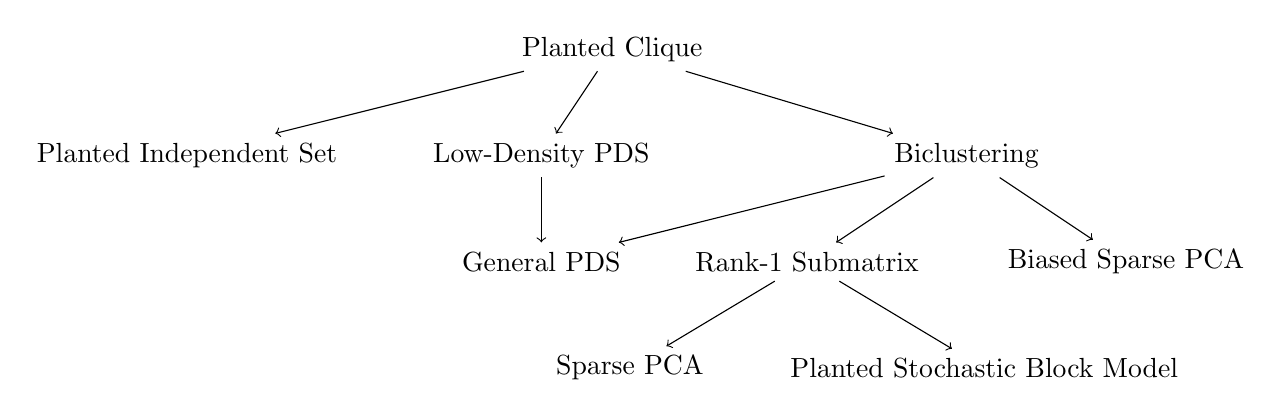
\begin{tikzpicture}[scale=0.45]
\node at (0, 0) (PC) {Planted Clique};
\node at (-12, -3) (PIS) {Planted Independent Set};
\node at (-2, -3) (SPDS) {Low-Density PDS};
\node at (10, -3) (BC) {Biclustering};
\node at (-2, -6) (PDS) {General PDS};
\node at (5.5, -6) (ROS) {Rank-1 Submatrix};
\node at (14.5, -6) (BSPCA) {Biased Sparse PCA};
\node at (0.5, -9) (SPCA) {Sparse PCA};
\node at (10.5, -9) (PSBM) {Planted Stochastic Block Model};

\draw[->] (PC) -- (PIS);
\draw[->] (PC) -- (SPDS);
\draw[->] (PC) -- (BC);
\draw[->] (SPDS) -- (PDS);
\draw[->] (BC) -- (PDS);
\draw[->] (BC) -- (BSPCA);
\draw[->] (BC) -- (ROS);
\draw[->] (ROS) -- (SPCA);
\draw[->] (ROS) -- (PSBM);
\end{tikzpicture}
\caption{Graph of average-case reductions for detection problems showing tight statistical-computational gaps given the planted clique conjecture.}
\end{figure*}

The aim of this paper is threefold: (1) to demonstrate that a web of average-case reductions between problems with statistical-computational gaps is feasible even for showing strong computational lower bounds; (2) to introduce a number of new techniques for reductions between problems; and (3) to fully characterize the computationally hard regime of several natural problems. The graph of our reductions is shown in Figure 1. Our new lower bounds are as follows.
\begin{itemize}
\item \textbf{Planted Independent Set:} We show tight lower bounds for recovering a planted independent set of size $k$ in a sparse Erd\H{o}s-R\'{e}nyi graph of size $n$ with edge density $\tilde{\Theta}(n^{-\alpha})$.
\item \textbf{Planted Dense Subgraph:} If $p > q$ are the edge densities inside and outside of the community, we show the first lower bounds for the general regime $q = \tilde{\Theta}(n^{-\alpha})$ and $p - q = \tilde{\Theta}(n^{-\gamma})$ where $\gamma \ge \alpha$, matching the lower bounds predicted in \cite{chen2016statistical}. Our lower bounds apply to a deterministic community size $k$, resolving a question raised in \cite{hajek2015computational}.
\item \textbf{Biclustering:} We show lower bounds for Gaussian biclustering as a simple hypothesis testing problem to detect a uniformly at random planted flat $k \times k$ submatrix. Our alternative reduction matches the barriers in \cite{ma2015computational}, where a computational lower bound was shown for a composite hypothesis testing variant of biclustering. We show hardness for the natural simple hypothesis testing problem where the $k \times k$ submatrix is chosen uniformly at random and has equal entries.
\item \textbf{Sparse Rank-1 Submatrix:} We show that general rank-1 submatrix detection has a different computational threshold from biclustering when $k \gg \sqrt{n}$. Surprisingly, we are able to obtain tight lower bounds matching these different detection thresholds with different reductions from planted clique.
\item \textbf{Sparse PCA:} We give a reduction between rank-1 submatrix and sparse PCA to obtain tight lower bounds in the less sparse regime $k \gg \sqrt{n}$, when the spectral algorithm is optimal over the SDP. This yields the first tight characterization of a computational barrier for sparse PCA over an entire parameter regime. We also give an alternate reduction recovering the lower bounds of \cite{berthet2013complexity} and \cite{gao2017sparse} in the canonical simple hypothesis testing variant of sparse PCA.
\item \textbf{Biased Sparse PCA:} We show that any assumption on the sparse principal component having a constant fraction more or fewer positive entries than negative entries yields a detection-recovery gap that is not present in sparse PCA. 
\item \textbf{Planted Stochastic Block Model:} Parallel to the difference between biclustering and rank-1 submatrix when $k \gg \sqrt{n}$, we introduce a sparse analogue of the stochastic block model and show that detection in this model is much harder than in planted dense subgraph when $k \gg \sqrt{n}$.
\end{itemize}
Our lower bounds for planted independent set, the general regime of planted dense subgraph, rank-1 submatrix, sparse PCA when $k \gg \sqrt{n}$, biased sparse PCA and the planted stochastic block model are novel. As previously mentioned, lower bounds for sparse PCA when $k \ll \sqrt{n}$, for biclustering and for planted dense subgraph in the sparsest regime were previously known. In each of these cases, we strengthen the existing lower bounds to the apply to the canonical generative model. We show computational lower bounds for simple vs. simple hypothesis testing in all cases other than for sparse PCA, rank-1 submatrix and the planted stochastic block model all in the regime $k \gg \sqrt{n}$. This is a consequence of our underlying reduction technique, reflection cloning, and appears unavoidable given our methods. However, we do show that the distribution we reduce to is in some sense close to the canonical generative model.

Our results demonstrate that, despite the delicate nature of average-case reductions, using natural problems as intermediates can often be beneficial as in reductions between deterministic problems. Our main technical contribution is to introduce four cloning techniques -- planted clique cloning, Poisson cloning, Gaussian cloning and reflection cloning -- that maintain the level of signal in an instance of a problem while increasing the size of its planted structure. The main idea behind Poisson and Gaussian cloning is to map edges of a graph to independent samples from these distributions and to algorithmically use distributional tricks to produce larger graphs while maintaining independence. Poisson cloning and Gaussian cloning lead to two very different parameter scalings, which when combined fully characterize general planted dense subgraph. Reflection cloning is a more randomness-efficient variant of Gaussian cloning that we use to show sharper lower bounds for certain problems. We also introduce new techniques for reductions to sparse PCA, including a connection between sparse PCA and rank-1 submatrix. We give algorithms matching our lower bounds and identify the information-theoretic limits of the models we introduce in Section 9.

\subsection{Hardness Results from an Algorithmic Perspective}

\begin{figure*}[t!]
\centering
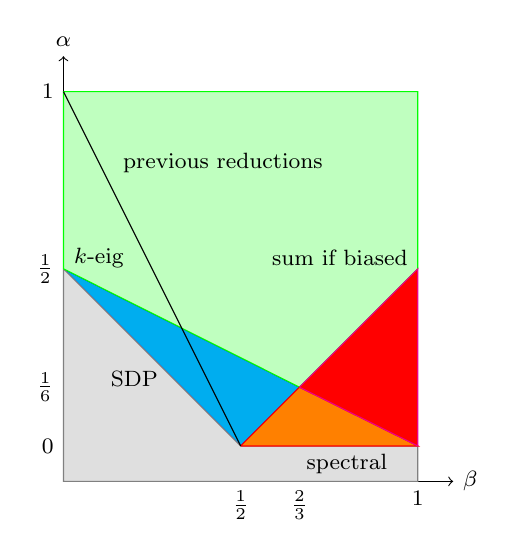
\begin{tikzpicture}[scale=0.45]
\tikzstyle{every node}=[font=\footnotesize]
\def\xmin{0}
\def\xmax{11}
\def\ymin{-1}
\def\ymax{11}

\draw[->] (\xmin,\ymin) -- (\xmax,\ymin) node[right] {$\beta$};
\draw[->] (\xmin,\ymin) -- (\xmin,\ymax) node[above] {$\alpha$};

\node at (5, -1) [below] {$\frac{1}{2}$};
\node at (6.66, -1) [below] {$\frac{2}{3}$};
\node at (10, -1) [below] {$1$};
\node at (0, 0) [left] {$0$};
\node at (0, 10) [left] {$1$};
\node at (0, 5) [left] {$\frac{1}{2}$};
\node at (0, 1.67) [left] {$\frac{1}{6}$};

\filldraw[fill=cyan, draw=blue] (0, 5) -- (6.66, 1.66) -- (5, 0) -- (0, 5);
\filldraw[fill=gray!25, draw=gray] (0, 5) -- (5, 0) -- (10, 0) -- (10, -1) -- (0, -1) -- (0, 5);
\filldraw[fill=green!25, draw=green] (0, 5) -- (6.66, 1.66) -- (10, 5) -- (10, 10) -- (0, 10) -- (0, 5);
\filldraw[fill=orange, draw=red] (5, 0) -- (6.66, 1.66) -- (10, 0) -- (5, 0);
\filldraw[fill=red, draw=magenta] (6.66, 1.66) -- (10, 5) -- (10, 0) -- (6.66, 1.66);
\draw (5, 0) -- (0, 10);

\node at (2, 1.9) {SDP};
\node at (1, 5.3) {$k$-eig};
\node at (8, -0.5) {spectral};
\node at (7.8, 5.3) {sum if biased};
\node at (4.5, 8) {previous reductions};
\end{tikzpicture}
\caption{Algorithms for Sparse PCA with $d = \Theta(n)$, $k = \tilde{\Theta}(n^\beta)$ and $\theta = \tilde{\Theta}(n^{-\alpha})$.}
\end{figure*}


In this section, we motivate our computational lower bounds and techniques using algorithms for sparse PCA as an example. Consider the detection problem for sparse PCA where either $X_1, X_2, \dots, X_n$ are sampled i.i.d. from $N(0, I_d)$ or are sampled i.i.d. from $N(0, I_d + \theta vv^\top)$ where $v$ is chosen uniformly at random from all $k$-sparse unit vectors with entries equal to $\pm 1/\sqrt{k}$. The task is to detect which of the two distributions the samples originated from. For now assume that $d = \Theta(n)$. Now consider the following four algorithms:
\begin{enumerate}
\item \textbf{Semidefinite Programming:} Form the empirical covariance matrix $\hat{\Sigma} = \frac{1}{n} \sum_{i = 1}^n X_i X_i^\top$ and solve the convex program
\begin{align*}
\max_Z \quad &\text{Tr}\left(\hat{\Sigma} Z\right) \\
\text{s.t.} \quad &\text{Tr}(Z) = 1, |Z|_1 \le k, Z \succeq 0
\end{align*}
As shown in \cite{berthet2013complexity}, thresholding the resulting maximum solves the detection problem as long as $\theta = \tilde{\Omega}(\sqrt{k^2/n})$.
\item \textbf{Spectral Algorithm:} Threshold the maximum eigenvalue of $\hat{\Sigma}$. If the data are sampled from $N(0, I_d)$, then the largest eigenvalue is with high probability at most
$$\lambda_{\text{max}}(\hat{\Sigma}) \le \frac{d}{n} + \sqrt{\frac{d}{n}} + 1 + o(1)$$
by standard bounds on the singular values of random Gaussian matrices. Since $d = \Theta(n)$, this algorithm succeeds as long as $\theta = \Omega(1)$. This algorithm was considered in \cite{krauthgamer2015semidefinite}.
\item \textbf{Sum Test:} Sum the entries of $\hat{\Sigma}$ and threshold the absolute value of the sum. If $v$ has sum exactly zero, then this test will not succeed. However, if we assume that $\hat{\Sigma}$ has even 51\% of its nonzero entries of one sign, then this test succeeds if $\theta = \tilde{\Omega}(\sqrt{n}/k)$.
\item \textbf{$k$-Sparse Eigenvalue:} Compute and threshold the $k$-sparse unit vector $u$ that maximizes $u^\top \hat{\Sigma} u$. This can be found by finding the largest eigenvector of each $k \times k$ principal submatrix of $\hat{\Sigma}$. Note that this takes exponential time. It was shown in \cite{berthet2013complexity} that this succeeds as long as $\theta = \tilde{\Omega}(\sqrt{k/n})$.
\end{enumerate}
The boundaries at which these algorithms begin to succeed are shown in Figure 2 for the regime $k = \tilde{\Theta}(n^\beta)$ and $\theta = \tilde{\Theta}(n^{-\alpha})$. The computational lower bound mapping to $\theta \approx k^2/n$ in \cite{berthet2013complexity} and \cite{gao2017sparse} is also drawn. As shown, the only point in the parameter diagram for which it matches an algorithmic upper bound is $\alpha = 0$ and $\beta = 1/2$, corresponding to when $\theta = \tilde{\Theta}(1)$ and $k = \tilde{\Theta}(\sqrt{n})$.

For general sparse PCA with $d = \Theta(n)$, the optimal algorithm is the SDP up until $k = \Theta(\sqrt{n})$, at which point the spectral algorithm has stronger guarantees. This algorithmic transition at $k = \Theta(\sqrt{n})$ is characteristic of all of the problems we consider. For the biased variant of sparse PCA where the sum test succeeds, then the sum test always does strictly better than the spectral algorithm. Furthermore, the biased variant ceases to have a statistical computational gap around $k = \Theta(n^{2/3})$. While the sum test yields an improved algorithm for detection, unlike the other three algorithms considered above, it does not translate into an algorithm for recovering the support of the sparse component. Given a conjecture about recovery in planted dense subgraph, we show that the best recovery algorithm for biased sparse PCA can only match the guarantees of the spectral algorithm. Thus the biased variant induces a detection-recovery gap when $k \gg \sqrt{n}$. We show that the disappearance of a statistical computation gap at $k = \Theta(n^{2/3})$ and a detection-recovery gap when $k \gg \sqrt{n}$ are features of the problems we consider that admit a sum test. These are biased sparse PCA, planted independent set, planted dense subgraph and biclustering. The techniques PC cloning, Poisson cloning and Gaussian cloning are all intended to capture these effects under different parameter scalings tailored to each problem.

In contrast, rank-1 submatrix, planted stochastic block model and sparse PCA do not admit a sum test. They have no detection-recovery gap and retain their statistical-computational gap for all sparsities $k$. We show tight hardness for these problems in the regime $k \gg \sqrt{n}$, where the spectral algorithm becomes optimal, using reflection cloning. Our results are the first planted clique lower bounds showing tight hardness in a regime where spectral is the optimal algorithm. It is somewhat surprising that the planted clique conjecture can tightly capture these very different phenomena for different problems, which demonstrates its usefulness as an average-case hardness assumption. While the sum test, spectral algorithm and semidefinite program all have equivalent guarantees up to logarithmic factors for planted clique, reductions from planted clique can be used to show hardness for problems for which this is not true.

\subsection{Prior Work on Statistical-Computational Gaps and PC Reductions}

Mention Montanari paper on Gaussian hidden clique

The Planted Clique problem is by far the most often used conjecturally hard problem for understanding computational barriers in statistics problems. In this problem one observes a sample from the Erd\"{o}s-R\'{e}nyi random graph ensemble on $N$ nodes, but only after a fully connected subgraph (clique) on $k$ nodes has been placed somewhere. The objective is to find the clique or, as shown equivalent by \cite{alon2007testing}, to determine whether or not a clique has been placed at all. All known efficient algorithms fail for cliques of size $k=o(\sqrt{N})$ despite considerable effort by the community (see, e.g., \cite{alon1998finding,deshpande2015finding}), yet a planted clique of size $k = (2+\epsilon)\log_2 N$ can be detected with high probability by enumerating over all possible size $k$ subsets of nodes. In light of this, the \emph{Planted Clique Hypothesis} presumes that algorithms running in time polynomial in $N$ can reliably detect the presence of a planted clique only if $k = \Omega(\sqrt{ N})$. Some evidence for the hardness of Planted Clique is provided in \cite{feldman2013statistical}, \cite{deshpande2015improved}, \cite{barak2016nearly}.

A succession of papers showed lower bounds for planted clique ultimately leading to a nearly tight lower bound for constant-degree SOS relaxations \cite{raghavendra2015tight, meka2015sum, deshpande2015improved, hopkins2016integrality, barak2016nearly}. SDP and degree-4 SOS lower bound have also been shown for sparse PCA \cite{krauthgamer2015semidefinite, ma2015sum}. In the recent work of \cite{hopkins2017power}, spectral and SOS algorithms were compared for problems with hidden sparse structure, including many that we consider here, and constant-degree SOS lower bounds were shown for sparse and tensor PCA. Tight computational lower bounds have also been shown in the statistical query model for planted clique and planted random $k$-SAT \cite{feldman2012statistical, feldman2015complexity}. A new meta-algorithm based on low-degree polynomials was recently proposed for community detection and shown to achieve the conjectured computational-statistical gap for the $k$-block stochastic block model \cite{hopkins2017bayesian}.

Mention sum of squares and SDP lower bound papers in one paragraph and mention PC reduction papers in another. List papers giving algorithms that solve planted clique down to $k = \Theta(\sqrt{n})$. Discuss the statistical-computational gap for PC in detail here. Give some references on average-case complexity in general (Impagliazzo and Trevisan references). Remark that hidden structure SOS paper shows lower bounds for the sparse spiked Wigner model, which is different from the spiked covariance model. It is a symmetric variant of the $\textsc{ROS}$ we consider here.

Also mention average-case reductions in the context of learning theory (e.g. see Daniely's paper)

Question: Should we include the spiked Wigner mode (possibly instead of ROS) in our problem formulations? Does the diagonal yield issues here? It seems like we possibly show a lower bound for the spiked Wigner model as well.

Papers to cite: \cite{hopkins2015tensor}, \cite{montanari2015limitation}, \cite{gao2015minimax}, \cite{bubeck2016testing}, \cite{dharmawansa2014joint}, \cite{ma2015volume}, \cite{perry2016optimality}, \cite{chen2016statistical}, \cite{flammarion2016optimal}, \cite{arias2016distribution}, \cite{d2007direct}, \cite{alon1998finding}, \cite{addario2010combinatorial}, \cite{arias2015detecting}, \cite{d2008optimal}, \cite{el2010information}. Look for papers from the past year? Cite SOS literature. Cite all existing PC reductions (see Hajek-Wu-Xu PDS paper and others for these references).

\cite{shalev2012using,berthet2013complexity,zhang2014lower,hardt2014computational,ma2015computational,hajek2015computational,ma2015sum,wang2016average,wang2016statistical,cai2015computational,chen2016statistical}

\cite{montanari2015limitation}

NOTE: Look through Banks et al. paper on information theoretic limits, Montanari papers (esp. on the limitations of spectral methods) and look through info limits for recovering a hidden community. Try to make sure that have information-theoretic lower bounds (and diagrams in general) correct for all problem formulations here. Also look for other generative models and places our results may have meaning. Would be great to get more results almost for free. Look through papers referenced in reductions in Section 3 and notes in the papers for ideas about notation, references, etc. Also see intros to these papers for intro ideas. Remember to mention NP-hardness of MLE's and how they yield nonconvex problems here.

\subsection{Notation}

In this paper, we adopt the following notational conventions. Let $\mL(X)$ denote the distribution law of a random variable $X$. Given a distribution $\mathbb{P}$, let $\mathbb{P}^{\otimes n}$ denote the distribution of $(X_1, X_2, \dots, X_n)$ where the $X_i$ are i.i.d. according to $\mathbb{P}$. Similarly, let $\mathbb{P}^{\otimes m \times n}$ denote the distribution on $\mathbb{R}^{m \times n}$ with i.i.d. entries distributed as $\mathbb{P}$. Given a finite or measurable set $\mathcal{X}$, let $\text{Unif}[\mathcal{X}]$ denote the uniform distribution on $\mathcal{X}$. Let $\TV$ and $\KL$ denote total variation distance and Kullback-Leibler divergence, respectively. Given a measurable set $\mathcal{X}$, let $\Delta(\mathcal{X})$ denote the set of all distributions $\pi$ on $\mathcal{X}$. If $\mathcal{X}$ is itself a set of distributions, we refer to $\Delta(\mathcal{X})$ as the set of priors on $\mathcal{X}$. Throughout the paper, $C$ refers to any constant independent of the parameters of the problem at hand and will be reused for different constants.

Let $N(\mu, \sigma^2)$ denote a normal random variable with mean $\mu$ and variance $\sigma^2$ when $\mu \in \mathbb{R}$ and $\sigma \in \mathbb{R}_{\ge 0}$. Let $N(\mu, \Sigma)$ denote a multivariate normal random vector with mean $\mu \in \mathbb{R}^d$ and covariance matrix $\Sigma$, where $\Sigma$ is a $d \times d$ positive semidefinite matrix. Let $\beta(x, y)$ denote a beta distribution with parameters $x, y > 0$ and let $\chi^2(k)$ denote a $\chi^2$-distribution with $k$ degrees of freedom. Let $\mathcal{B}_0(k)$ denote the set of all unit vectors $v \in \mathbb{R}^d$ with $\| v \|_0 \le k$. Let $[n] = \{1, 2, \dots, n\}$ and $\binom{[n]}{k}$ denote the set of all size $k$ subsets of $[n]$. Let $\mG_n$ denote the set of all simple graphs on vertex set $[n]$. Let the Orthogonal group on $\bR^{d \times d}$ be $\mO_d$. Let $\mathbf{1}_S$ denote the vector $v \in \mathbb{R}^n$ with $v_i = 1$ if $i \in S$ and $v_i = 0$ if $i \not \in S$ where $S \subseteq [n]$. For subsets $S \subseteq \mathbb{R}$, let $\mathbf{1}_S$ denote the indicator function of the set $S$. Let $\Phi$ denote the cumulative distribution of a standard normal random variable with $\Phi(x) = \int_{-\infty}^x e^{-t^2/2} dt$. Given a simple undirected graph $G$, let $V(G)$ and $E(G)$ denote its vertex and edge sets, respectively.

\section{Summary of Results}

\subsection{Problem Formulations}

% NOTES: Expand on history and references for each problem as you introduce it, check appropriate loss functions for recovery problems, do we need type I+II error tending to zero or just being bounded away from zero (same for loss and recovery)? Add to lists of papers mentioning each of the problems and survey interesting developments for each if you can. Should we consider support recovery only for consistency or do we want to consider loss functions? Would need to consider minimax convergence rates for loss functions? Make sure all of the times you reference the literature are exhaustive. Also maybe move some references and background to the introduction -- try to make this section just introduce generative models and give any history that wasn't relevant in the background section of the introduction? Is notion of loss in hardness conjectures correct? Maybe only have to give DKS gap conjecture (can derive BC gap conjecture from DKS)? Idea: state all recovery problems as recovering the support of the planted structure so as to avoid loss functions. Discuss these loss functions and recovering values given the support at the end of the paper? However, fundamentally, for SPCA and ROS the signal might not be strong enough across the support to permit exact support recovery. How do we deal with this? Probably need to deal with minimax rates for ROS and SPCA? Also, what about the fact that biclustering is not necessarily symmetric! Somewhat amazingly, this does not seem to be an issue going from PC to Biclustering and then to DKS (since will preserve symmetry? what about diagonals in the cloning? cite argument in other paper?) and is not an issue going from DKS to biclustering. In this section, you should also review what composite hypothesis testing is (you will need the prior formulation later anyways). May want to still discuss multiple spikes? This is a nontrivial generalization -- think about after. Also look at relevant papers to check for any relevant related models that we may be able to show hardness for.

In this section, we define the problems that we show computational lower bounds for and the conjectures on which these lower bounds are based. Each problem we consider has a natural parameter $n$, which typically denotes the number of samples or dimension of the data, and sparsity parameter $k$. Every parameter for each problem is implicitly a function of $n$, that grows or decays polynomially in $n$. For example, $k = k(n) = \tilde{\Theta}(n^{\beta})$ for some constant $\beta \in (0, 1)$ throughout the paper. For simplicity of notation, we do not write this dependence on $n$. The notation $a \gg b$ will denote $a$ growing polynomially faster in $n$ than $b$. We mostly will be concerned with the polynomial order of growth of each of the parameters and not with $\text{polylog}(n)$ factors. For each problem $\mP$, we consider both a detection task and a recovery task, which we denote by $\mP_D$ and $\mP_R$, respectively. In detection, the algorithm is given a set of observations and tasked with distinguishing between two hypotheses:
\begin{itemize}
\item a \emph{uniform} hypothesis $H_0$, under which observations are generated from the natural noise distribution for the problem; and
\item a \emph{planted} hypothesis $H_1$, under which observations are generated from the same noise distribution with a latent planted sparse structure.
\end{itemize}
In all of the detection problems we consider, $H_0$ is a simple hypothesis consisting of a single distribution and $H_1$ is either also simple or a composite hypothesis consisting of several distributions. We will abuse notation and refer to $H_1$ both as a hypothesis and as a set of distributions. An instance of a problem $\mP$ refers to an observation $X$. We denote the distribution of $X$ under $H_0$ and some $\bP \in H_1$ as $\mL_{H_0}(X)$ and $\mL_{\bP}(X)$, respectively. Given an observation $X$, a test $\phi(X) \to \{0, 1\}$ solves the detection problem if its Type I$+$II error satisfies that for some $\epsilon > 0$,
$$\bP_{H_0}[\phi(X) = 1] + \sup_{\bP \in H_1} \bP_{X \sim \bP}[\phi(X) = 0] < 1 - \epsilon \text{ as } n \to \infty.$$
We refer to the $\liminf$ of this quantity as $n \to \infty$ as the asymptotic Type I$+$II error. In recovery, the algorithm is given a set of observations generated from $H_1$ and the task is to recover the support of the latent planted sparse structure. An algorithm succeeds if its expected loss decays to zero as $n \to \infty$. An important feature of our setup is that the natural noise distribution for each problem remains fixed in $H_0$ and throughout $H_1$. In other words, our hardness results apply to algorithms that are allowed to make use of the specific features of a fixed natural noise distribution. In general, we aim to show lower bounds for simple hypotheses and otherwise as restrictive composite hypotheses as possible. Note that computational lower bounds for more restrictive $H_1$ are stronger results, implying hardness for algorithms with fewer guarantees.

We now formally define the detection and recovery variants of each problem we consider. Let $G(n, p)$ denote the distribution on the set $\mG_n$ of simple graphs on the vertex set $[n]$ where each pair of distinct vertices is joined by an edge independently with probability $p$. Let $G(n, p, S)$ where $S$ is a subset of $[n]$ denote the distribution on $\mG_n$ formed by sampling a graph from $G(n, p)$ and replacing the edges between pairs of vertices in $S$ with a clique. Let $G(n, k, p)$ be generated by selecting a size $k$ subset $S$ of $[n]$ uniformly at random and generating a sample from $G(n, p, S)$. The planted clique problem is defined as follows.

\paragraph{Planted Clique} The problem $\textsc{PC}(n, k, p)$ has variants:
\begin{itemize}
\item \emph{Detection}: Given observation of a graph $G \in \mG_n$, distinguish between the two hypotheses
$$H_0: G \sim G(n, p) \quad \text{and} \quad H_1 : G \sim G(n, k, p)$$
\item \emph{Recovery}: Given observation of a graph $G \sim G(n, k, p)$, recover the latent support of the clique exactly.
\end{itemize}

In \cite{alon2007testing}, it is shown that detection and recovery are equivalent for planted clique. We discuss this internal reduction further in Section 8. The variant of the planted clique conjecture we use in our lower bounds is stated below. Note that this variant only states that $\text{PC}_D(n, k)$ is hard when $k$ is polynomially less than $\sqrt{n}$ and conjectures that no polynomial-time test can achieve a Type I$+$II error asymptotically better than random guessing. It is widely conjectured that the PC detection problem remains hard as long as $k = o(\sqrt{n})$.

\paragraph{PC Conjecture} Fix some constant $p$. Suppose that $\{ \phi_n \}$ is a sequence of randomized polynomial time tests $\phi_n : \mG_n \to \{0, 1\}$ and $k_n$ is a sequence of positive integers satisfying that $\limsup_{n \to \infty} \log_n k_n < \frac{1}{2}$. Then if $G$ is an instance of $\textsc{PC}_D(n, k, p)$, it holds that
$$\liminf_{n \to \infty} \left( \bP_{H_0}\left[\phi_n(G) = 1\right] + \bP_{H_1}\left[\phi_n(G) = 0\right] \right) \ge 1.$$

Other than to show hardness for planted dense subgraph in the sparsest regime, we will only need the PC conjecture for $p = 1/2$. An interesting open problem is to show that the PC conjecture at $p = 1/2$ implies it for any fixed constant $p < 1/2$. Let $G_I(n, k, p)$ be the distribution resulting from planting a uniformly at random selected independent set of size $k$ in $G(n, p)$. We will generally consider the sparse regime of planted independent set with $p = \tilde{\Theta}(n^{-\alpha})$ for some $\alpha \in (0, 2)$. Note that planted independent set is equivalent to planted clique with density $1 - p$, but is the more natural formulation for detection in sparse graphs.

\paragraph{Planted Independent Set} The problem $\textsc{PIS}(n, k, p)$ has variants:
\begin{itemize}
\item \emph{Detection}: Given observation of a graph $G \in \mG_n$, distinguish between the two hypotheses
$$H_0: G \sim G(n, p) \quad \text{and} \quad H_1 : G \sim G_I(n, k, p)$$
\item \emph{Recovery}: Given observation of a graph $G \sim G_I(n, k, p)$, recover the latent support of the independent set exactly.
\end{itemize}

Let $G(n, p, q, S)$ where $S$ is a subset of $[n]$ be formed by including all edges between vertices in $S$ independently with probability $p$ and all other edges with probability $q$. Let $G(n, k, p, q)$ be the distribution resulting from choosing $S$ uniformly at random from all size $k$ subsets of $[n]$. We consider the general regime of planted dense subgraph in which $p - q$ is decaying at least as quickly as $q$. More precisely, we consider $q = \tilde{\Theta}(n^{-\alpha})$ and $p - q = \tilde{\Theta}(n^{-\gamma})$ where $\gamma \ge \alpha$ are both in $(0, 2)$.

\paragraph{Planted Dense Subgraph} The problem $\textsc{PDS}(n, k, p, q)$ has variants:
\begin{itemize}
\item \emph{Detection}: Given observation of a graph $G \in \mG_n$, distinguish between
$$H_0: G \sim G(n, q) \quad \text{and} \quad H_1 : G \sim G(n, k, p, q)$$
\item \emph{Recovery}: Given observation of a graph $G \sim G(n, k, p, q)$, recover the latent support of the planted dense subgraph exactly.
\end{itemize}

Biclustering has been considered in \cite{ma2015computational}, where computational lower bounds were shown assuming the PC conjecture for a composite hypothesis testing variant. Here we consider the simple vs. simple hypothesis testing variant of biclustering, leading to stronger computational lower bounds.

\paragraph{Biclustering} The problem $\textsc{BC}(n, k, \mu)$ has variants:
\begin{itemize}
\item \emph{Detection}: Given observation of a matrix $M \in \mathbb{R}^{n \times n}$, distinguish between
$$H_0: M \sim N(0, 1)^{\otimes n \times n} \quad \text{and} \quad H_1 : M \sim \mu \cdot A + N(0, 1)^{\otimes n \times n} \text{ where } A \sim \text{Unif}\left[\mathcal{M}_k\right]$$
where $\mathcal{M}_k \subseteq \mathbb{R}^{n \times n}$ is the set of sparse matrices supported on a $k \times k$ submatrix with each nonzero entry equal to $1$.
\item \emph{Recovery}: Given a matrix $M \sim \mu \cdot A + N(0, 1)^{\otimes n \times n}$ where $A \sim \text{Unif}\left[\mathcal{M}_k\right]$, recover the sets $S, T \subseteq [n]$ with $|S| = |T| = k$ such that $A$ is supported on the indices $S \times T$.
\end{itemize}

For rank-1 submatrix and sparse PCA, exact support recovery is only possible under a $\beta$-min condition -- where entries of the planted rank-1 submatrix or sparse principal component are assumed to be non-negligible. To overcome this issue, we take unit vectors in these two problems from the set
$$\mathcal{V}_{d,k} = \left\{ v \in \mathbb{S}^{d-1}  : k - \frac{k}{\log k} \le \| v \|_0 \le k \text{ and } |v_i| \ge \frac{1}{\sqrt{k}} \text{ for } i \in \text{supp}(v) \right\}$$
The function $\log k$ can be replaced by any sub-polynomially growing function. Note that $\mathcal{V}_{d, k}$ is the set of unit vectors with entries nearly uniform in absolute value and with support of size approximately $k$.

\paragraph{Rank-1 Submatrix} The problem $\textsc{ROS}(n, k, \mu)$ has variants:
\begin{itemize}
\item \emph{Detection}: Given observation of a matrix $M \in \mathbb{R}^{n \times n}$, distinguish between
$$H_0: M \sim N(0, 1)^{\otimes n \times n} \quad \text{and} \quad H_1 : M \sim \mu \cdot rc^\top + N(0, 1)^{\otimes n \times n} \text{ where } r, c \in \mathcal{V}_{n, k}$$
\item \emph{Recovery}: Given a matrix $M \sim \mu \cdot rc^\top + N(0, 1)^{\otimes n \times n}$ where $r, c \in \mathcal{V}_{n, k}$, output the latent supports $\text{supp}(r)$ and $\text{supp}(c)$.
\end{itemize}

Since its introduction in \cite{johnstoneSparse04}, sparse PCA has appeared in several forms in statistics and computer science literature. Here, we consider the most common generative model for sparse PCA -- the spiked covariance model.

\paragraph{Sparse PCA} The problem $\textsc{SPCA}(n, k, d, \theta)$ has variants:
\begin{itemize}
\item \emph{Detection}: Given observation of $n$ samples $X_1, X_2, \dots, X_n \in \mathbb{R}^d$, distinguish between
\begin{align*}
&H_0: X_1, X_2, \dots, X_n \sim N(0, I_d)^{\otimes n} \quad \text{and} \\
&H_1 : X_1, X_2, \dots, X_n \sim N\left(0, I_d + \theta vv^\top\right)^{\otimes n} \text{ where } v \in \mathcal{V}_{d, k}
\end{align*}
\item \emph{Recovery}: Given $n$ samples $X_1, X_2, \dots, X_n \sim N(0, I_d + \theta vv^\top)^{\otimes n}$ where $v \in\mathcal{V}_{d, k}$, output the latent support $\text{supp}(v)$.
\end{itemize}

In order to reveal a subtlety in the complexity of sparse PCA, we introduce a variant of the spiked covariance model with an additional promise. In particular, $v$ is restricted to the set $\mathcal{BV}_{d, k}$ of vectors in $\mathcal{V}_{d,k}$ with some overall positive or negative bias. Formally, if $\| v \|_0^+$ denotes the number of positive entries of $v$ then
$$\mathcal{BV}_{d, k} = \left\{ v \in \mathcal{V}_{d, k} : \| v \|_0^+ \ge \left( \frac{1}{2} + \delta \right) k \text{ or } \| v \|_0^+ \le \left( \frac{1}{2} - \delta \right) k \right\}$$
where $\delta > 0$ is an arbitrary constant that will remain fixed throughout the paper. The purpose of considering this biased variant is to reveal a subtlety in the complexity of sparse PCA. We will show that ordinary sparse PCA has the same thresholds for detection and recovery, while the additional promise that $v \in \mathcal{BV}_{d, k}$ induces a detection-recovery gap given the PDS gap conjecture. The moral reason for this gap is a simple sum test that can detect $H_1$ but not recover $v$ when $v \in \mathcal{V}_{d, k}$. We describe this test in more detail in Section 9.

\paragraph{Biased Sparse PCA} The problem $\textsc{SPCA}(n, k, d, \theta)$ has variants:
\begin{itemize}
\item \emph{Detection}: Given observation of $n$ samples $X_1, X_2, \dots, X_n \in \mathbb{R}^d$, distinguish between
\begin{align*}
&H_0: X_1, X_2, \dots, X_n \sim N(0, I_d)^{\otimes n} \quad \text{and} \\
&H_1 : X_1, X_2, \dots, X_n \sim N\left(0, I_d + \theta vv^\top\right)^{\otimes n} \text{ where } v \in \mathcal{BV}_{d, k}
\end{align*}
\item \emph{Recovery}: Given $n$ samples $X_1, X_2, \dots, X_n \sim N(0, I_d + \theta vv^\top)^{\otimes n}$ where $v \in\mathcal{BV}_{d, k}$, output the latent support $\text{supp}(v)$.
\end{itemize}

We also consider a simple vs. simple hypothesis testing variants of sparse and biased sparse PCA. In $\textsc{USPCA}(n, k, d, \theta)$, under $H_1$, the latent principal component $v$ is chosen uniformly at random from all $k$-sparse unit vectors with nonzero entries equal to $\pm 1/\sqrt{k}$. Similarly, define $\textsc{UBSPCA}(n, k, d, \theta)$ to select $v$ uniformly at random from all $k$-sparse unit vectors with nonzero entries equal to $1/\sqrt{k}$. We show lower bounds for these simple hypothesis testing models matching the results of \cite{gao2017sparse}.

Let $G_B(n, k, q, \rho)$ denote the set of distributions on $\mG_n$ generated a graph $G$ as follows. Fix any two positive integers $k_1$ and $k_2$ satisfying that
$$\frac{k}{2} - k^{1-\delta} \le k_1, k_2 \le \frac{k}{2} + k^{1 - \delta}$$
where $\delta > 0$ is a small constant that will remained fixed throughout the paper. Let $S = [k_1]$ and $T = [k_1+k_2]\backslash [k_1]$. Then generate the edges of $G$ independently as follows.
\begin{enumerate}
\item include edges within $S$ or within $T$ with probability at least $q + \rho$;
\item include edges between $S$ and $T$ with probability at most $q - \rho$; and
\item include all other edges with probability $q$.
\end{enumerate}
Then permute the vertices of $G$ according to a permutation selected uniformly at random. The communities of the graph are defined to be the images of $S$ and $T$ under this permutation. Note that $G_B(n, k, q, \rho)$ defines a set of distributions since $k_1$ and $k_2$ are permitted to vary and the edges between $S$ and $T$ are included independently with a probability at least $q + \rho$ for each edge. Thus given the random permutation, $G$ is distributed as an inhomogeneous random graph with independent edges. The planted stochastic block model is now defined as follows.

\paragraph{Planted Stochastic Block Model} The problem $\textsc{PSBM}(n, k, q, \rho)$ has variants:
\begin{itemize}
\item \emph{Detection}: Given observation of a graph $G \in \mG_n$, distinguish between
$$H_0: G \sim G(n, q) \quad \text{and} \quad H_1 : G \sim \bP \quad \text{ for some } \quad \bP \in G_B(n, k, q, \rho)$$
\item \emph{Recovery}: Given observation of a graph $G \sim \bP$ for some $\bP \in G_B(n, k, q, \rho)$, recover the latent supports of the two communities exactly.
\end{itemize}

A phenomenon observed in \cite{cai2015computational} and \cite{hajek2015computational} is that many problems with sum tests appear to have detection-recovery gaps in the regime where $k \gg \sqrt{n}$. This gap is most easily formulated for general PDS, as was conjectured in \cite{chen2016statistical}, where it was shown that convex relaxations of the MLE for recovery in PDS and BC have this detection-recovery gap.

\paragraph{PDS Recovery Conjecture} If $G$ is an instance of $\textsc{PDS}_R(n, k, p, q)$ with
$$\liminf_{n \to \infty} \log_n k > \frac{1}{2} \quad \text{and} \quad \limsup_{n \to \infty} \log_n \left(\frac{k^2(p-q)^2}{q(1-q)} \right) < 1$$
then there is no sequence of randomized polynomial-time tests $\phi_n : \mG_n \to \binom{[n]}{k}$ such that $\phi_n(G)$ correctly outputs the vertices in the latent planted dense subgraph with probability at least $\epsilon$ for any fixed $\epsilon > 0$. \\

This conjecture essentially asserts that the threshold of $n/k^2$ on the signal $\frac{(p-q)^2}{q(1 - q)}$ of an instance of PDS holds for recovery. In contrast, our results show that the tight detection threshold for PDS given the PC conjecture is lower, at $n^2/k^4$. We will use this conjecture to establish similar detection-recovery gaps for biased sparse PCA and biclustering. We note that a related detection-recovery gap for BC was shown in \cite{cai2015computational}. The same lower bound was established for strong recovery algorithms that bicluster for all subgaussian noise distributions assuming hardness of planted clique for a different distribution on random graphs than Erd\H{o}s-Reny\'{i}.

\subsection{Our Results}

\begin{figure*}[t!]
\centering

\subfigure[$\textsc{PIS}(n, k, q)$ and $\textsc{PDS}(n, k, p, q)$ with $k = \tilde{\Theta}(n^{\beta})$ and $p = cq = \tilde{\Theta}(n^{-\alpha})$]{
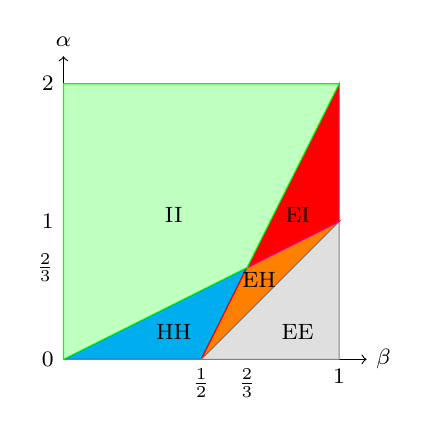
\begin{tikzpicture}[scale=0.35]
\tikzstyle{every node}=[font=\footnotesize]
\def\xmin{0}
\def\xmax{11}
\def\ymin{0}
\def\ymax{11}

\draw[->] (\xmin,\ymin) -- (\xmax,\ymin) node[right] {$\beta$};
\draw[->] (\xmin,\ymin) -- (\xmin,\ymax) node[above] {$\alpha$};

\node at (5, 0) [below] {$\frac{1}{2}$};
\node at (6.66, 0) [below] {$\frac{2}{3}$};
\node at (10, 0) [below] {$1$};
\node at (0, 0) [left] {$0$};
\node at (0, 10) [left] {$2$};
\node at (0, 3.33) [left] {$\frac{2}{3}$};
\node at (0, 5) [left] {$1$};

\filldraw[fill=cyan, draw=blue] (0,0) -- (5, 0) -- (6.66, 3.33) -- (0, 0);
\filldraw[fill=orange, draw=red] (5, 0) -- (6.66, 3.33) -- (10, 5) -- (5, 0);
\filldraw[fill=gray!25, draw=gray] (5, 0) -- (10, 5) -- (10, 0) -- (0, 0) -- (0, 0) -- (5, 0);
\filldraw[fill=red, draw=magenta] (6.66, 3.33) -- (10, 5) -- (10, 10) -- (6.66, 3.33);
\filldraw[fill=green!25, draw=green] (0, 0) -- (6.66, 3.33) -- (10, 10) -- (0, 10) -- (0, 0);

\node at (4, 1) {HH};
\node at (8.5, 1) {EE};
\node at (7.1, 2.9) {EH};
\node at (8.5, 5.25) {EI};
\node at (4, 5.25) {II};
\end{tikzpicture}}
\quad
\subfigure[Example of $\textsc{PDS}(n, k, p, q)$ with $q = \tilde{\Theta}(n^{-\alpha})$ and $p - q = \tilde{\Theta}(n^{-\gamma})$ with $\gamma = 5\alpha/4$]{
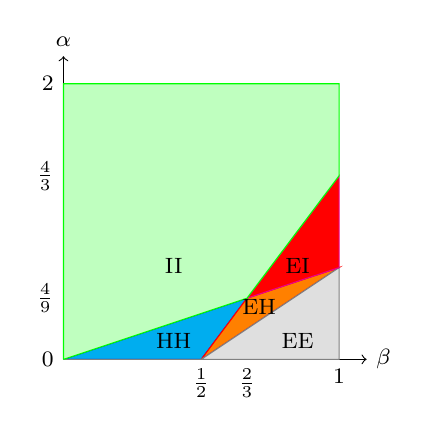
\begin{tikzpicture}[scale=0.35]
\tikzstyle{every node}=[font=\footnotesize]
\def\xmin{0}
\def\xmax{11}
\def\ymin{0}
\def\ymax{11}

\draw[->] (\xmin,\ymin) -- (\xmax,\ymin) node[right] {$\beta$};
\draw[->] (\xmin,\ymin) -- (\xmin,\ymax) node[above] {$\alpha$};

\node at (5, 0) [below] {$\frac{1}{2}$};
\node at (6.66, 0) [below] {$\frac{2}{3}$};
\node at (10, 0) [below] {$1$};
\node at (0, 0) [left] {$0$};
\node at (0, 10) [left] {$2$};
\node at (0, 2.22) [left] {$\frac{4}{9}$};
\node at (0, 6.66) [left] {$\frac{4}{3}$};

\filldraw[fill=cyan, draw=blue] (0,0) -- (5, 0) -- (6.66, 2.22) -- (0, 0);
\filldraw[fill=orange, draw=red] (5, 0) -- (6.66, 2.22) -- (10, 3.33) -- (5, 0);
\filldraw[fill=gray!25, draw=gray] (5, 0) -- (10, 3.33) -- (10, 0) -- (0, 0) -- (0, 0) -- (5, 0);
\filldraw[fill=red, draw=magenta] (6.66, 2.22) -- (10, 3.33) -- (10, 6.66) -- (6.66, 2.22);
\filldraw[fill=green!25, draw=green] (0, 0) -- (6.66, 2.22) -- (10, 6.66) -- (10, 10) -- (0, 10) -- (0, 0);

\node at (4, 0.66) {HH};
\node at (8.5, 0.66) {EE};
\node at (7.1, 1.92) {EH};
\node at (8.5, 3.4) {EI};
\node at (4, 3.4) {II};
\end{tikzpicture}}
\quad
\subfigure[$\textsc{PSBM}(n, k, q, \rho)$ with $q = \tilde{\Theta}(1)$ and $\rho = \tilde{\Theta}(n^{-\alpha})$]{
\centering
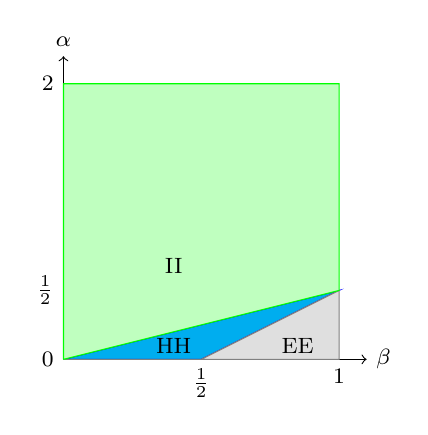
\begin{tikzpicture}[scale=0.35]
\tikzstyle{every node}=[font=\footnotesize]
\def\xmin{0}
\def\xmax{11}
\def\ymin{0}
\def\ymax{11}

\draw[->] (\xmin,\ymin) -- (\xmax,\ymin) node[right] {$\beta$};
\draw[->] (\xmin,\ymin) -- (\xmin,\ymax) node[above] {$\alpha$};

\node at (5, 0) [below] {$\frac{1}{2}$};
\node at (10, 0) [below] {$1$};
\node at (0, 0) [left] {$0$};
\node at (0, 10) [left] {$2$};
\node at (0, 2.5) [left] {$\frac{1}{2}$};

\filldraw[fill=cyan, draw=blue] (0,0) -- (5, 0) -- (10, 2.5) -- (0, 0);
\filldraw[fill=gray!25, draw=gray] (5, 0) -- (10, 2.5) -- (10, 0) -- (0, 0) -- (0, 0) -- (5, 0);
\filldraw[fill=green!25, draw=green] (0, 0) -- (10, 2.5) -- (10, 10) -- (0, 10) -- (0, 0);

\node at (4, 0.5) {HH};
\node at (8.5, 0.5) {EE};
\node at (4, 3.4) {II};
\end{tikzpicture}}
\quad
\subfigure[$\textsc{BC}(n, k, \mu)$ with $\mu = \tilde{\Theta}(n^{-\alpha})$]{
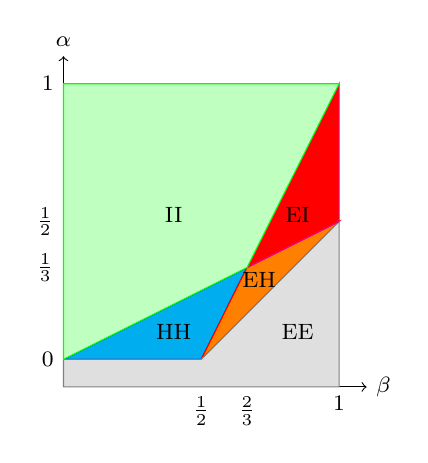
\begin{tikzpicture}[scale=0.35]
\tikzstyle{every node}=[font=\footnotesize]
\def\xmin{0}
\def\xmax{11}
\def\ymin{-1}
\def\ymax{11}

\draw[->] (\xmin,\ymin) -- (\xmax,\ymin) node[right] {$\beta$};
\draw[->] (\xmin,\ymin) -- (\xmin,\ymax) node[above] {$\alpha$};

\node at (5, -1) [below] {$\frac{1}{2}$};
\node at (6.66, -1) [below] {$\frac{2}{3}$};
\node at (10, -1) [below] {$1$};
\node at (0, 0) [left] {$0$};
\node at (0, 10) [left] {$1$};
\node at (0, 3.33) [left] {$\frac{1}{3}$};
\node at (0, 5) [left] {$\frac{1}{2}$};

\filldraw[fill=cyan, draw=blue] (0,0) -- (5, 0) -- (6.66, 3.33) -- (0, 0);
\filldraw[fill=orange, draw=red] (5, 0) -- (6.66, 3.33) -- (10, 5) -- (5, 0);
\filldraw[fill=gray!25, draw=gray] (5, 0) -- (10, 5) -- (10, -1) -- (0, -1) -- (0, 0) -- (5, 0);
\filldraw[fill=red, draw=magenta] (6.66, 3.33) -- (10, 5) -- (10, 10) -- (6.66, 3.33);
\filldraw[fill=green!25, draw=green] (0, 0) -- (6.66, 3.33) -- (10, 10) -- (0, 10) -- (0, 0);

\node at (4, 1) {HH};
\node at (8.5, 1) {EE};
\node at (7.1, 2.9) {EH};
\node at (8.5, 5.25) {EI};
\node at (4, 5.25) {II};
\end{tikzpicture}}
\quad
\subfigure[$\textsc{ROS}(n, k, \mu)$ with $\frac{\mu}{k} = \tilde{\Theta}(n^{-\alpha})$]{
\centering
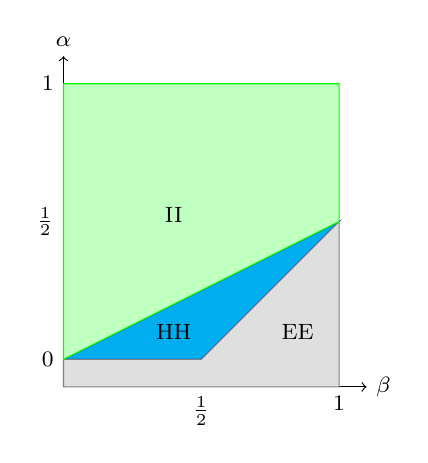
\begin{tikzpicture}[scale=0.35]
\tikzstyle{every node}=[font=\footnotesize]
\def\xmin{0}
\def\xmax{11}
\def\ymin{-1}
\def\ymax{11}

\draw[->] (\xmin,\ymin) -- (\xmax,\ymin) node[right] {$\beta$};
\draw[->] (\xmin,\ymin) -- (\xmin,\ymax) node[above] {$\alpha$};

\node at (5, -1) [below] {$\frac{1}{2}$};
\node at (10, -1) [below] {$1$};
\node at (0, 0) [left] {$0$};
\node at (0, 10) [left] {$1$};
\node at (0, 5) [left] {$\frac{1}{2}$};

\filldraw[fill=cyan, draw=blue] (0,0) -- (5, 0) -- (10, 5) -- (0, 0);
\filldraw[fill=gray!25, draw=gray] (5, 0) -- (10, 5) -- (10, -1) -- (0, -1) -- (0, 0) -- (5, 0);
\filldraw[fill=green!25, draw=green] (0, 0) -- (10, 5) -- (10, 10) -- (0, 10) -- (0, 0);

\node at (4, 1) {HH};
\node at (8.5, 1) {EE};
\node at (4, 5.25) {II};
\end{tikzpicture}}

\subfigure[$\textsc{SPCA}(n, k, d, \theta)$ with $d = \Theta(n)$ and $\theta = \tilde{\Theta}(n^{-\alpha})$]{
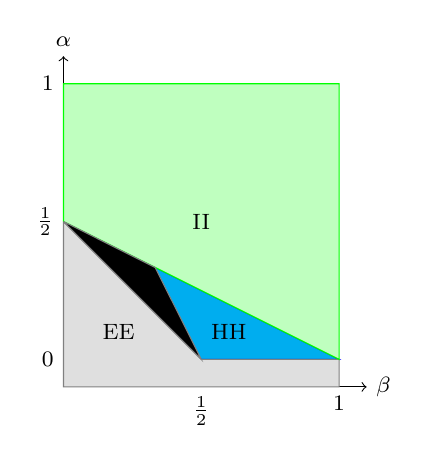
\begin{tikzpicture}[scale=0.35]
\tikzstyle{every node}=[font=\footnotesize]
\def\xmin{0}
\def\xmax{11}
\def\ymin{-1}
\def\ymax{11}

\draw[->] (\xmin,\ymin) -- (\xmax,\ymin) node[right] {$\beta$};
\draw[->] (\xmin,\ymin) -- (\xmin,\ymax) node[above] {$\alpha$};

\node at (5, -1) [below] {$\frac{1}{2}$};
\node at (10, -1) [below] {$1$};
\node at (0, 0) [left] {$0$};
\node at (0, 10) [left] {$1$};
\node at (0, 5) [left] {$\frac{1}{2}$};

\filldraw[fill=cyan, draw=blue] (0, 5) -- (10, 0) -- (5, 0) -- (0, 5);
\filldraw[fill=gray!25, draw=gray] (0, 5) -- (5, 0) -- (10, 0) -- (10, -1) -- (0, -1) -- (0, 5);
\filldraw[fill=green!25, draw=green] (0, 5) -- (10, 0) -- (10, 10) -- (0, 10) -- (0, 5);
\filldraw[fill=black, draw=gray] (0, 5) -- (3.33, 3.33) -- (5, 0) -- (0, 5);
\node at (6, 1) {HH};
\node at (2, 1) {EE};
\node at (5, 5) {II};
\end{tikzpicture}}
\quad
\subfigure[$\textsc{BSPCA}(n, k, d, \theta)$ with $d = \Theta(n)$ and $\theta = \tilde{\Theta}(n^{-\alpha})$]{
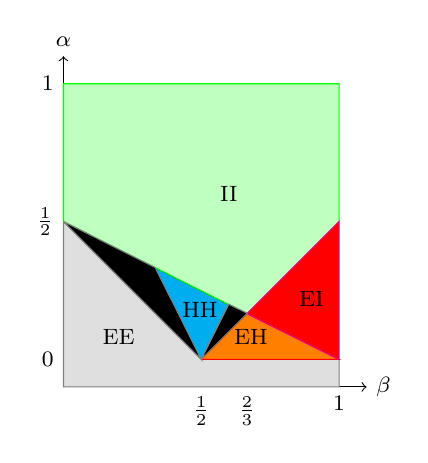
\begin{tikzpicture}[scale=0.35]
\tikzstyle{every node}=[font=\footnotesize]
\def\xmin{0}
\def\xmax{11}
\def\ymin{-1}
\def\ymax{11}

\draw[->] (\xmin,\ymin) -- (\xmax,\ymin) node[right] {$\beta$};
\draw[->] (\xmin,\ymin) -- (\xmin,\ymax) node[above] {$\alpha$};

\node at (5, -1) [below] {$\frac{1}{2}$};
\node at (6.66, -1) [below] {$\frac{2}{3}$};
\node at (10, -1) [below] {$1$};
\node at (0, 0) [left] {$0$};
\node at (0, 10) [left] {$1$};
\node at (0, 5) [left] {$\frac{1}{2}$};

\filldraw[fill=cyan, draw=blue] (0, 5) -- (6.66, 1.66) -- (5, 0) -- (0, 5);
\filldraw[fill=gray!25, draw=gray] (0, 5) -- (5, 0) -- (10, 0) -- (10, -1) -- (0, -1) -- (0, 5);
\filldraw[fill=green!25, draw=green] (0, 5) -- (6.66, 1.66) -- (10, 5) -- (10, 10) -- (0, 10) -- (0, 5);
\filldraw[fill=orange, draw=red] (5, 0) -- (6.66, 1.66) -- (10, 0) -- (5, 0);
\filldraw[fill=red, draw=magenta] (6.66, 1.66) -- (10, 5) -- (10, 0) -- (6.66, 1.66);
\filldraw[fill=black, draw=gray] (0, 5) -- (3.33, 3.33) -- (5, 0) -- (0, 5);
\filldraw[fill=black, draw=gray] (5, 0) -- (6, 2) -- (6.67, 1.67) -- (5, 0);

\node at (2, 0.8) {EE};
\node at (6, 6) {II};
\node at (4.95, 1.8) {HH};
\node at (6.8, 0.8) {EH};
\node at (9, 2.2) {EI};
\end{tikzpicture}}
\caption{Parameter regimes by problem plotted as signal vs. sparsity. Sparsity is parameterized as $k = \tilde{\Theta}(n^{\beta})$. The first label characterizes detection and the second characterizes recovery in the regime. In Easy (E) regimes, there is a polynomial-time algorithm. In Hard (H) regimes, the PC or PDS gap conjecture implies that there is no polynomial-time algorithm. In Impossible (I) regimes, the task is information-theoretically impossible. Hardness in the black regions for SPCA and BSPCA are open.}
\end{figure*}

% NOTES: Check to see where we actually need $\gg$ for parameter regimes and when it is simply an inequality $\ge$. Need to check this throughout the discussion in the paper! This is a nontrivial subtlety that you should get right everywhere. Question: Do we need to say we are just showing $d = \Theta(n)$? Can we say something like $d = \Omega(n)$ instead? In this section, discuss all of the ways to think about the parameters of sparse PCA and what our results mean from the sample complexity viewpoint. Give 3D diagram for general PDS?

In this paper, our aim is to establish tight characterizations of the statistical-computational gaps for the problems formulated in the previous section. Each problem has three regimes for each of its detection and recovery variants. In the easy regime, there is a polynomial-time algorithm for the task. In the hard regime, the PC or PDS conjecture implies that there is no polynomial-time algorithm but there is an inefficient algorithm solving the task. In the impossible regime, the task is information-theoretically impossible. Our results complete the hardness picture for each of these problems other than sparse PCA when $k \ll \sqrt{n}$. Our results are informally stated below and depicted visually in Figure 3. Here $a \lesssim b$ denotes $a \le b$ up to polylogarithmic factors in $n$.

\begin{theorem}[Informal Main Theorem]
Given the PC and PDS recovery conjectures, the detection and recovery variants of the problems in Section 2.1 have easy, hard and impossible parameter regions as indicated below. For each problem, let $k$ be in the regime $k = \tilde{\Theta}(n^{\beta})$ where $\beta \in (0, 1)$ is a constant.
\begin{enumerate}
\item $\textsc{PIS}_D(n, k, q)$ and $\textsc{PDS}_D(n, k, cq, q)$ in the regime $q = \tilde{\Theta}(n^{-\alpha})$ for some fixed $\alpha \in [0, 1)$ and constant $c > 1$, has regions
\begin{align*}
&\bullet \, \, \mathbf{Easy} \left\{ \begin{array}{ll} q \gtrsim \frac{n^2}{k^4} &\text{if } k \gtrsim \sqrt{n} \end{array} \right. \quad \quad  \bullet \, \, \mathbf{Hard} \left\{ \begin{array}{ll} q \gtrsim \frac{1}{k} &\text{if } k \ll \sqrt{n} \\ \frac{n^2}{k^4} \gg q \gtrsim \frac{1}{k} &\text{if } \sqrt{n} \lesssim k \ll n^{2/3} \end{array} \right. \\
& \bullet \, \, \mathbf{Impossible} \left\{ \begin{array}{ll} q \ll \frac{1}{k} &\text{if } k \ll n^{2/3} \\ q \ll \frac{n^2}{k^4} &\text{if } k \gtrsim n^{2/3} \end{array} \right.
\end{align*}
\item $\textsc{PIS}_R(n, k, q)$ and $\textsc{PDS}_R(n, k, cq, q)$ in the regime $q = \tilde{\Theta}(n^{-\alpha})$ for some fixed $\alpha \in [0, 1)$ and constant $c > 1$, has regions
\begin{align*}
&\bullet \, \, \mathbf{Easy} \left\{ \begin{array}{ll} q \gtrsim \frac{n}{k^2} &\text{if } k \gtrsim \sqrt{n} \end{array} \right. \quad \quad  \bullet \, \, \mathbf{Hard} \left\{ \begin{array}{ll} q \gtrsim \frac{1}{k} &\text{if } k \ll \sqrt{n} \\ \frac{n}{k^2} \gg q \gtrsim \frac{1}{k} &\text{if } \sqrt{n} \lesssim k \ll n^{2/3} \end{array} \right. \\
& \bullet \, \, \mathbf{Impossible} \left\{ \begin{array}{ll} q \ll \frac{1}{k} \end{array} \right.
\end{align*}
\item $\textsc{PDS}_D(n, k, p, q)$ in the regime $p > q$, $q = \tilde{\Theta}(n^{-\alpha})$ and $p - q = \tilde{\Theta}(n^{-\gamma})$ for some fixed $\alpha, \gamma \in [0, 1)$ with $\gamma \ge \alpha$, has regions
\begin{align*}
&\bullet \, \, \mathbf{Easy} \left\{ \begin{array}{ll} \frac{(p - q)^2}{q(1 -q)} \gtrsim \frac{n^2}{k^4} &\text{if } k \gtrsim \sqrt{n} \end{array} \right. \quad \quad  \bullet \, \, \mathbf{Hard} \left\{ \begin{array}{ll} \frac{(p - q)^2}{q(1 -q)} \gtrsim \frac{1}{k} &\text{if } k \ll \sqrt{n} \\ \frac{n^2}{k^4} \gg \frac{(p - q)^2}{q(1 -q)} \gtrsim \frac{1}{k} &\text{if } \sqrt{n} \lesssim k \ll n^{2/3} \end{array} \right. \\
& \bullet \, \, \mathbf{Impossible} \left\{ \begin{array}{ll} \frac{(p - q)^2}{q(1 -q)} \ll \frac{1}{k} &\text{if } k \ll n^{2/3} \\ \frac{(p - q)^2}{q(1 -q)} \ll \frac{n^2}{k^4} &\text{if } k \gtrsim n^{2/3} \end{array} \right.
\end{align*}
\item$\textsc{PDS}_R(n, k, p, q)$ in the regime $p > q$, $q = \tilde{\Theta}(n^{-\alpha})$ and $p - q = \tilde{\Theta}(n^{-\gamma})$ for some fixed $\alpha, \gamma \in [0, 1)$ with $\gamma \ge \alpha$, has regions
\begin{align*}
&\bullet \, \, \mathbf{Easy} \left\{ \begin{array}{ll} \frac{(p - q)^2}{q(1 -q)} \gtrsim \frac{n}{k^2} &\text{if } k \gtrsim \sqrt{n} \end{array} \right. \quad \quad  \bullet \, \, \mathbf{Hard} \left\{ \begin{array}{ll} \frac{(p - q)^2}{q(1 -q)} \gtrsim \frac{1}{k} &\text{if } k \ll \sqrt{n} \\ \frac{n}{k^2} \gg \frac{(p - q)^2}{q(1 -q)} \gtrsim \frac{1}{k} &\text{if } \sqrt{n} \lesssim k \ll n^{2/3} \end{array} \right. \\
& \bullet \, \, \mathbf{Impossible} \left\{ \begin{array}{ll} \frac{(p - q)^2}{q(1 -q)} \ll \frac{1}{k} \end{array} \right.
\end{align*}
\item $\textsc{PSBM}_D(n, k, q, \rho)$ and $\textsc{PSBM}_R(n, k, q, \rho)$ in the regime $q = \theta(1)$ and $\rho = \tilde{\Theta}(n^{-\alpha})$ for some fixed $\alpha \in [0, 1)$, has regions
\begin{align*}
&\bullet \, \, \mathbf{Easy} \left\{ \begin{array}{ll} \rho \gtrsim \frac{\sqrt{n}}{k} &\text{if } k \gtrsim \sqrt{n} \end{array} \right. \quad \quad  \bullet \, \, \mathbf{Hard} \left\{ \begin{array}{ll} \rho \gtrsim \frac{1}{\sqrt{k}} &\text{if } k \ll \sqrt{n} \\ \frac{\sqrt{n}}{k} \gg \rho \gtrsim \frac{1}{\sqrt{k}} &\text{if } k \gtrsim \sqrt{n} \end{array} \right. \\
& \bullet \, \, \mathbf{Impossible} \left\{ \begin{array}{ll} \rho \ll \frac{1}{\sqrt{k}} \end{array} \right.
\end{align*}
\item $\textsc{BC}_D(n, k, \mu)$ in the regime $\mu = \tilde{\Theta}(n^{-\alpha})$ for some fixed $\alpha \in [0, 1)$, has regions
\begin{align*}
&\bullet \, \, \mathbf{Easy} \left\{ \begin{array}{ll} \mu \gtrsim 1 &\text{if } k \ll \sqrt{n} \\ \mu \gtrsim \frac{n}{k^2} &\text{if } k \gtrsim \sqrt{n} \end{array} \right. \quad \quad  \bullet \, \, \mathbf{Hard} \left\{ \begin{array}{ll} 1 \gg \mu \gtrsim \frac{1}{\sqrt{k}} &\text{if } k \ll \sqrt{n} \\ \frac{n}{k^2} \gg \mu \gtrsim \frac{1}{\sqrt{k}} &\text{if } \sqrt{n} \lesssim k \ll n^{2/3} \end{array} \right. \\
& \bullet \, \, \mathbf{Impossible} \left\{ \begin{array}{ll} \mu \ll \frac{1}{\sqrt{k}} &\text{if } k \ll n^{2/3} \\ \mu \ll \frac{n}{k^2} &\text{if } k \gtrsim n^{2/3} \end{array} \right.
\end{align*}
\item $\textsc{BC}_R(n, k, \mu)$ in the regime $\mu = \tilde{\Theta}(n^{-\alpha})$ for some fixed $\alpha \in [0, 1)$, has regions
\begin{align*}
&\bullet \, \, \mathbf{Easy} \left\{ \begin{array}{ll} \mu \gtrsim 1 &\text{if } k \ll \sqrt{n} \\ \mu \gtrsim \frac{\sqrt{n}}{k} &\text{if } k \gtrsim \sqrt{n} \end{array} \right. \quad \quad  \bullet \, \, \mathbf{Hard} \left\{ \begin{array}{ll} 1 \gg \mu \gtrsim \frac{1}{\sqrt{k}} &\text{if } k \ll \sqrt{n} \\ \frac{\sqrt{n}}{k} \gg \mu \gtrsim \frac{1}{\sqrt{k}} &\text{if } k \gtrsim \sqrt{n} \end{array} \right. \\
& \bullet \, \, \mathbf{Impossible} \left\{ \begin{array}{ll} \mu \ll \frac{1}{\sqrt{k}} \end{array} \right.
\end{align*}
\item $\textsc{ROS}_D(n, k, \mu)$ and $\textsc{ROS}_R(n, k, \mu)$ in the regime $\mu = \tilde{\Theta}(n^{-\alpha})$ for some fixed $\alpha \in [0, 1)$, have regions
\begin{align*}
&\bullet \, \, \mathbf{Easy} \left\{ \begin{array}{ll} \mu \gtrsim k &\text{if } k \ll \sqrt{n} \\ \mu \gtrsim \sqrt{n} &\text{if } k \gtrsim \sqrt{n} \end{array} \right. \quad \quad  \bullet \, \, \mathbf{Hard} \left\{ \begin{array}{ll} k \gg \mu \gtrsim \sqrt{k} &\text{if } k \ll \sqrt{n} \\ \sqrt{n} \gg \mu \gtrsim \sqrt{k} &\text{if } k \gtrsim \sqrt{n} \end{array} \right. \\
& \bullet \, \, \mathbf{Impossible} \left\{ \begin{array}{ll} \mu \ll \sqrt{k} \end{array} \right.
\end{align*}
\item $\textsc{SPCA}_D(n, k, d, \theta)$, $\textsc{SPCA}_R(n, k, d, \theta)$ and $\textsc{BSPCA}_R(n, k, d, \theta)$ in the regime $d = \Theta(n)$ and $\theta = \tilde{\Theta}(n^{-\alpha})$ for some $\alpha \in [0, 1)$, have regions
\begin{align*}
&\bullet \, \, \mathbf{Easy} \left\{ \begin{array}{ll} \theta \gtrsim \frac{k}{\sqrt{n}} &\text{if } k \ll \sqrt{n} \\ \theta \gtrsim 1 &\text{if } k \gtrsim \sqrt{n} \end{array} \right. \quad \quad  \bullet \, \, \mathbf{Hard} \left\{ \begin{array}{ll} \frac{k^2}{n} \gg \theta \gtrsim \sqrt{\frac{k}{n}} &\text{if } k \ll \sqrt{n} \\ 1 \gg \theta \gtrsim \sqrt{\frac{k}{n}} &\text{if } k \gtrsim \sqrt{n} \end{array} \right. \\
& \bullet \, \, \mathbf{Impossible} \left\{ \begin{array}{ll} \theta \ll \sqrt{\frac{k}{n}} \end{array} \right.
\end{align*}
\item $\textsc{BSPCA}_D(n, k, d, \theta)$ in the regime $d = \Theta(n)$ and $\theta = \tilde{\Theta}(n^{-\alpha})$ for some $\alpha \in [0, 1)$, has regions
\begin{align*}
&\bullet \, \, \mathbf{Easy} \left\{ \begin{array}{ll} \theta \gtrsim \frac{k}{\sqrt{n}} &\text{if } k \ll \sqrt{n} \\ \theta \gtrsim \frac{\sqrt{n}}{k} &\text{if } k \gtrsim \sqrt{n} \end{array} \right. \quad \quad  \bullet \, \, \mathbf{Hard} \left\{ \begin{array}{ll} \frac{k^2}{n} \gg \theta \gtrsim \sqrt{\frac{k}{n}} &\text{if } k \ll \sqrt{n} \\ \frac{n}{k^2} \gg \theta \gtrsim \sqrt{\frac{k}{n}} &\text{if } \sqrt{n} \lesssim k \ll n^{2/3} \end{array} \right. \\
&\bullet \, \, \mathbf{Impossible} \left\{ \begin{array}{ll} \theta \ll \sqrt{\frac{k}{n}} &\text{if } k \ll n^{2/3} \\ \theta \ll \frac{\sqrt{n}}{k} &\text{if } k \gtrsim n^{2/3} \end{array} \right.
\end{align*}
\end{enumerate}
\end{theorem}

Note that this gives a complete characterization of the easy, hard and impossible regions for all of the problems we consider other than sparse PCA and biased sparse PCA. The SDP relaxation of the MLE for sparse PCA was shown in \cite{berthet2013optimal} to succeed if $d = \Theta(n)$ and $k \ll n^{1/2 - \delta}$ down to the signal level of $\theta \approx k/\sqrt{n}$, which is generally conjectured to be optimal. There is a gap between the lower bounds we prove here, which match those of \cite{berthet2013optimal} and \cite{gao2017sparse} and this conjecturally optimal threshold when $k \ll \sqrt{n}$. There is also a gap for biased sparse PCA detection when $k \gg \sqrt{n}$. These gaps are depicted as the black region in figures 2(f) and 2(g). Showing tight hardness for sparse PCA for any parameters $k \ll \sqrt{n}$ remains an interesting open problem.

In Figure 3 and Theorem 1, we depict the implications of our hardness results for $\textsc{SPCA}$ and $\textsc{BSPCA}$ in the case where $d = \Theta(n)$ for simplicity. Our hardness results extend mildly beyond this regime, but not tightly. However, we remark that the assumptions $d = \Theta(n)$ or $d = \Omega(n)$ have become commonplace in the literature on lower bounds for sparse PCA. The reductions from PC to sparse PCA in \cite{berthet2013complexity}, \cite{wang2016statistical} and \cite{gao2017sparse} construct hard instances that are only tight when $d = \Omega(n)$. The sum of squares lower bounds for sparse PCA in \cite{ma2015sum} and \cite{hopkins2017power} also are in the regime $d = \Theta(n)$. The SOS lower bounds in \cite{hopkins2017power} are actually for the spiked Wigner model, a symmetric version of our formulation of rank-1 submatrix. In proving planted clique lower bounds for planted stochastic block model in Section 6, we also show lower bounds for the spiked Wigner model as an intermediate step.

\subsection{Strength of Algorithmic Guarantees in Computational Lower Bounds}

Discuss how formulations preclude trivial monotonicity reductions e.g. despite same $\theta \approx 1$ threshold when $k \gg \sqrt{n}$ for SPCA, seem to need reflection cloning

VERY VERY IMPORTANT: Figure out how to phrase asymptotic regimes and ensure do not have trivial monotonicity in our composite hypotheses. Figure out whether or not Haar rotation, Philippe's paper and Ma-Gao-Zhou all show suboptimal bounds of $\theta \ll k^2/n$ when $k \ll \sqrt{n}$. Decide whether to mark the regime in the hardness diagram open or solved. Potentially use this to sell the fact that show hardness for the whole spectral line. Make sure to pay homage generously to the papers by Ma-Wu, Hajek-Wu-Xu, Berthet-Rigollet and Ma-Gao-Zhou. This work builds on those heavily.

Give complete characterization, important -- not like SPCA reductions so far.

SOME REMARKS HERE NOW INCORRECT: Several of the lower and upper bounds that compose Theorem 1 have been established previously in the literature. In \cite{ma2015computational}, all three of the regimes for $\textsc{BC}_D$ are identified assuming the PC conjecture. Along with tight upper bounds for the recovery problems, these lower bounds imply the hard regimes of $\textsc{BC}_R$, $\textsc{ROS}_D$ and $\textsc{ROS}_R$ when $k \ll \sqrt{n}$. Furthermore, the hard regimes of $\textsc{SPCA}_D$ and $\textsc{SPCA}_R$ for $k \ll \sqrt{n}$ are established in \cite{gao2017sparse}. Our contributions to the bounds implicit in Theorem 1 are mostly in the regimes where $k \gtrsim \sqrt{n}$. As shown in Theorem 1 and Figure 1, the problems we consider undergo interesting changes on entering the regime $k \gtrsim \sqrt{n}$. The line defining the boundary of the hard regime seems to always change and the problems $\textsc{BC}$, $\textsc{DKS}$ and $\textsc{BSPCA}$ conjecturally develop detection-recovery gaps. We introduce a new reduction technique we call reflection cloning to capture the sharper hardness of $\textsc{SPCA}_D$ and $\textsc{ROS}_D$ when $k \gtrsim \sqrt{n}$ in comparison to the problems $\textsc{BC}_D$ and $\textsc{DKS}_D$ in this regime. This is discussed in Section 4. We also introduce a new connection between $\textsc{BC}$ to $\textsc{SPCA}$ based on random rotations that establishes computational lower bounds for $\textsc{SPCA}$ and $\textsc{BSPCA}$ over the entire parameter space, including giving an alternate reduction matching the results of \cite{gao2017sparse}. This is discussed in Section 5.

We also give a slightly modified reduction proving the hardness results of \cite{ma2015computational} for $\textsc{BC}_D$ in Section 4, that will motivate our reduction from PC to $\textsc{ROS}_D$ using reflection cloning. In Section 4, we deduce the hardness of $\textsc{DKS}_D$ from $\textsc{BC}_D$ and show that the DKS conjecture implies the BC conjecture using truncated kernels. We also discuss internal reductions between different variants of problems in Section 6, including reductions between detection, recovery and estimating the signal given its support. In Section 6, we also discuss issues of discretization and the fact that computational procedures will only store continuous random variables up to a certain precision. In Section 7, we discuss the algorithms information-theoretic thresholds needed to complete the picture laid out in Theorem 1 and Figure 1.

Potentially merge all detection definitions in the previous section into a list to compress the previous section? Do this at the end.

Discuss the fact that $\mathcal{V}_{d, k}$ is not monotonic for increasing $k$ unlike $\mathcal{B}_0(k)$. Thus we do not implicitly assume that an algorithm cannot make use of the fact that the signal is spread.

Mostly restrict previous section to definitions and history about problems, save comments for this section

IMPORTANT NOTE: Make it clearer what the problem definitions actually mean since everything in this paper is fundamentally asymptotic for clarity of exposition. A problem such as $\textsc{SPCA}(n, k, d, \theta)$ includes all sequences of instantiations $\textsc{SPCA}(n, k_n, d_n, \theta_n)$ such that for each other parameter such as $\theta_n$, we have that $\lim_{n \to \infty} \log_n \theta_n = \lim_{n \to \infty} \log_n \theta(n)$. State what this formally means in terms of hypothesis classes. For our reductions, this means that if we do not map to exactly $\theta = n^{-\alpha}$ say, but rather to a sequence of $\theta_n$'s converging in the right sense to $\theta = n^{-\alpha}$ then this is fine. Relate this to previous reductions in the literature so does not seem like making things easier. Wait to include this in the write-up so can at the end of the day assume as little as possible. Overall, try to make the discussion of hypotheses, asymptotic regimes, etc. as clean, motivated and succinct as possible. Do not distract from the meat of the paper. Use the notation $\tilde{\Theta}$ to denote parameters converging in the sense you care about and define here.

IMPORTANT: Look at Ma-Wu and Hajek-Wu-Xu for background on how to set things up, look at their intros, intro of Montanari's paper and Chen-Xu intro for references and inspiration. Give all hardness theorems in terms of rates of decay (give informal in beginning with just parameters). Read some of Hajek-Wu-Xu for structure inspiration. Discuss strength of previous computational lower bounds here.

QUESTION: Are the polynomial dominating terms the strongest guarantees we can get?

This section is the natural place to give asymptotic assumptions etc. Give a formal definition for what it means to solve a problem in a certain regime and then give an example with PDS for clarity.

We take the stronger approach as in Ma-Wu and Hajek-Wu-Xu for showing hardness for weak blackboxes. Our blackboxes are only assumed to work in a particular asymptotic parameter regime (i.e. particular polynomial term in the rates of decay or growth of parameters). We avoid hidden robustness or monotonicity in our composite hypotheses. When our reductions require composite $H_1$ usually is consequence of reduction type -- room for improvement. Compare to blackbox assumptions in other reduction papers. Mention how some reductions (all but PSBM although don't know support size in ROS, SPCA, BSPCA) show hardness for blackboxes that need to know certain parameters.

Our approach is more typical of average-case complexity where even basic questions of monotonicity are nontrivial. Mention random CSPs open question of Impagliazzo.

NOTE: Indicate in this section exactly what we reduce to and what stronger hardness results actually hold i.e. our results persist when you assume the latent sets include planted vectors of constant absolute value, also if simple hypothesis with sparse support uniform over $\binom{[n]}{k}$. Can permute after. Should we give all problems in this formulation? Only ambiguity is $k$, which should be allowed to range over a region. Is $k$ the only parameter that needs to remain specified asymptotically (I think we can achieve convergence ratio to $1$)? Then can avoid all asymptotic notation and setup? This might be easiest. Put these remarks in a separate section?

Discuss monotonicity in sparse PCA formulations and the set $\mathcal{V}_{d, k}$. Comb through previous section and move all of this type of discussion here.

We remark that the problem formulations in this section are deliberately restricted to as few parameters as possible. It is possible to in many cases decouple or include additional parameters while preserving our hardness results. For example, the reductions yielding our computational lower bounds for biclustering and rank-1 submatrix remain valid if the observation matrix is permitted to be rectangular or have different sparsities along different dimensions, as considered in \cite{cai2015computational}.

VERY IMPORTANT NOTE: Must make sure that SPCA and ROS are not monotone in $k \gg \sqrt{n}$ otherwise the result is meaningless, as $k \approx \sqrt{n}$ is trivially a hard instance with the same threshold (since the threshold is constant). Should formulate these two problems so that recovery is also possible (instances with min condition). Want to actually be saying that spreading out the signal does not help here (note that this is not difficult on just sparse PCA, reflecting cloning along one dimension obviously works). Check for more issues like this of bad formulations, rendering your results less meaningful. For now, go with making magnitudes nearly uniform and make the composite hypothesis over all $k'$ with $k'/k \to 1$. Can explain that assume each magnitude at least $Ck^{-1/2}$ to make recovery well-defined and problems at different values of $k$ actually different. Note that more particular composite hypotheses $H_1$ require stronger lower bounds. Note where we show hardness that is stronger than the set we give in $H_1$. For now will be able to map exactly by stating that (will need something better than this)
$$\mathcal{V}_k = \left\{ v \in \mathcal{B}_0(k) : |v_i| \ge \frac{1}{C\sqrt{k}} \text{ for } i \in \text{supp}(v) \right\}$$
$$\mathcal{V}_k = \left\{ v  : \| v\|_2 = 1, k - o(k) \le \| v \|_0 \le k + o(k), |v_i| \ge \frac{1}{C\sqrt{k}} \text{ for } i \in \text{supp}(v) \right\}$$
for some constant $C$. Do remark that this means support size can be less than $k$. Define recovery as recovering the support. Now have overcome both issues. Also remark that this is the collection of nearly uniform magnitude sparse components. Will map to almost uniform in magnitude sparse components. Remark that these are thought to be the hardest instances of sparse PCA and uniform magnitude has been taken in the SOS literature. Do mention for transparency that have not been quite able to map exactly to uniform magnitude. Would like to be consistent across problems -- not have a monotone problem, then do not properly capture any algorithms that can somehow make use of the higher sparsity? Here there are none? Reasons three-fold: (1) capture different problems with different values of $k$; (2) permit support recovery; (3) give stronger lower bounds. In statement of results, give regime as well (even though state bounds with parameters) e.g. $\mu = \tilde{\Theta}(n^{-\alpha})$ for some fixed $\alpha > 0$. Give random permuting definition of planted stochastic block model. Discuss how reflection cloning trick achieves tighter tradeoff and is the only non-``lossy" cloning method. It seems necessary to achieve the tight lower bound for planted stochastic block model.

\section{Average-Case Reductions for Statistical Problems}

% NOTES: State all of the general setup here in terms of composite hypothesis testing problems, maybe define what an instance of a detection problem is earlier (using the priors definition, definitely need to make this clear somewhere). Define special type of hypothesis testing problem called a detection problem, explain abuse of notation of $H_1$ as a set of distributions and for laws. IMPORTANT NOTE: Before proceeding, sort out all of your notation right now! Indicate all abuses of notation, conventions for simplicity, etc. IMPORTANT NOTE: Before proceed with write-up, read Wu-Cai paper on Sparse submatrix detection and read Gao-Ma-Zhou paper showing hardness for spiked covariance, Wu-Cai paper may give a natural way to generalize to multiple spikes or submatrices.

The typical approach to show computational lower bounds for detection problems is to reduce an instance of one problem to a random object close in total variation distance to an instance of another problem in randomized polynomial time. More precisely, let $\mP$ and $\mP'$ be detection problems and $X$ and $Y$ be instances of $\mP$ and $\mP'$, respectively. Suppose we are given a polynomial-time computable map $\phi$ taking an object $\phi(X)$ with total variation distance to $Y$ decaying to zero simultaneously under each of $H_0$ and $H_1$. Then any algorithm that can distinguish $H_0$ and $H_1$ for $\mP'$ in polynomial time when applied to $\phi(X)$ also distinguishes $H_0$ and $H_1$ for $\mP$. Taking $\mP$ to be PC and $\mP'$ to be the problem of interest then yields a computational hardness result for $\mP'$ conditional on the PC conjecture. The general idea in this approach is formalized in the following simple lemma.

\begin{lemma}
Let $\mP$ and $\mP'$ be detection problems with hypotheses $H_0, H_1, H_0', H_1'$ and let $X$ and $Y$ be instances of $\mP$ and $\mP'$, respectively. Suppose there is a polynomial time computable map $\phi$ satisfying
$$\TV\left(\mL_{H_0}(\phi(X)), \mL_{H_0'}(Y)\right) + \sup_{\bP \in H_1} \inf_{\pi \in \Delta(H_1')} \TV\left( \mL_{\bP}(\phi(X)), \int_{H_1'} \mL_{\bP'}(Y) d\pi(\bP') \right) \le \delta$$
If there is a polynomial time algorithm solving $\mP'$ with Type I$+$II error at most $\epsilon$, then there is a polynomial time algorithm solving $\mP$ with Type I$+$II error at most $\epsilon + \delta$.
\end{lemma}

\begin{proof}
Let $\psi$ be a polynomial time computable test function solving $\mP'$ with Type I$+$II error at most $\epsilon$. Note that for any observation $X$ of $\mP$, the value $\psi \circ \phi(X) \in \{0, 1\}$ can be computed in polynomial time. This is because the fact that $\phi(X)$ can be computed in polynomial time implies that $\phi(X)$ has size polynomial in the size of $X$. We claim that $\psi \circ \phi$ solves the detection problem $\mP'$. Now fix some distribution $\bP \in H_1$ and prior $\pi \in \Delta(H_1')$. By the definition of total variation,
\begin{align*}
\left| \bP_{H_0} \left[ \psi \circ \phi(X) = 1 \right] - \bP_{H_0'} \left[ \psi(Y) = 1 \right] \right| &\le \TV\left(\mL_{H_0}(\phi(X)), \mL_{H_0'}(Y)\right) \\
\left| \bP_{X \sim \bP} \left[ \psi \circ \phi(X) = 0 \right] - \int_{H_1'} \bP_{Y \sim \bP'} \left[ \psi(Y) = 0 \right] d\pi(\bP') \right| &\le \TV\left( \mL_{\bP}(\phi(X)), \int_{H_1'} \mL_{\bP'}(Y) d\pi(\bP') \right)
\end{align*}
Also note that since $\pi$ is a probability distribution,
$$\int_{H_1'} \bP_{Y \sim \bP'} \left[ \psi(Y) = 0 \right] d\pi(\bP') \le \sup_{\bP' \in H_1'} \bP_{Y \sim \bP'} \left[ \psi(Y) = 0 \right]$$
Combining these inequalities with the triangle inequality yields that
\begin{align*}
\bP_{H_0} \left[ \psi \circ \phi(X) = 1 \right] + \bP_{X \sim \bP} \left[ \psi \circ \phi(X) = 0 \right] \le \epsilon &+ \TV\left(\mL_{H_0}(\phi(X)), \mL_{H_0'}(Y)\right) \\
&+ \TV\left( \mL_{\bP}(\phi(X)), \int_{H_1'} \mL_{\bP'}(Y) d\pi(\bP') \right)
\end{align*}
Fixing $\bP$ and choosing the prior $\pi$ so that the second total variation above approaches its infimum yields that the right hand side above is upper bounded by $\epsilon + \delta$. The fact that this bound holds for all $\bP \in H_1$ proves the lemma.
\end{proof}

We remark that the second term in the total variation condition of Lemma 1 can be interpreted as ensuring that each distribution $\bP \in H_1$ is close to a distribution formed by taking a prior $\pi$ over the distributions in hypothesis $H_1'$. In light of this lemma, to reduce one problem to another it suffices to find such a map $\phi$. We now review several relevant techniques for constructing these maps $\phi$ from PC in the literature and outline our technical contributions.

\subsection{Berthet-Rigollet's Reduction for Distribution-Robust Sparse PCA}

NOTES: Here also mention reduction of Berthet et al. Explain how produce instances with $k \ll \sqrt{n}$ and how this relates to $R_0$ which enforces $k \le d^{0.49}$? Is this interpretation correct? Also discuss other Berthet-Rigollet paper here (annals of stats paper)

\subsection{Truncated Kernels and Ma-Wu's Reduction for Biclustering}

NOTES: Mention other paper here?

\subsection{Hajek-Wu-Xu's Reduction for PDS}

NOTES: Here also mention reduction of Hajek-Wu-Xu

\subsection{Gao-Ma-Zhou's Reduction for Sparse PCA}

NOTES: Note seems as though his theorem applies to cases where $k \gg \sqrt{n}$ but is suboptimal (extension is simple and amounts to through away some of the $n$ samples). Why does Gao-Ma-Zhou appear to need $k \gg n^{1/4}$? What is the significance of this? Do we implicitly need this?

\subsection{Our Techniques}

\paragraph{PC, Poisson and Gaussian Cloning} Begin with an instance of planted clique. Idea is want to increase $k$ while maintaining the signal and independence. Idea of Hajek-Wu-Xu to blow up -- very complicated analysis, requiring the dense subgraph size to be random. Main technical issue is blowing up diagonal entries. Rather than do a blow up all at once, we attempt an iterative blow up -- hoping this will simplify the analysis and permit stronger guarantees. Graph edges are distributed as Bernoulli's and can preserve signal as in PC cloning. Diagonals become the issue but randomly permuting the vertices can obscure planted entries on the blow up of the diagonal. Not difficult to show that this approach require $p/q \to 1$ when mapping to PDS to do exactly. So would need to approximately map at each step. However, this yields total variation errors that appear to grow quickly. Our insight is that indicator random variables of whether or not edges are present are often not the right random variables. Rather than accumulate errors at each step, we map to a distribution with a distributional trick allowing each step to be exact. We map to Poisson and Gaussians. These achieve very different parameter scaling because Gaussians do not necessarily have means on the order of their variances while Poisson variables do. Tricks are Poisson thinning and that rotations of independent Gaussian vectors are still independent, allowing signal to be spread. Give picture illustrating blow up techniques in general. The idea of replacing Bernoulli's with these distributions proves powerful, yielding simple reductions with simple analyses closing the complexity of PDS in the most general regime and recovering prior results. Also gives biclustering lower bounds as a by product. Indicate sections where these appear.

\paragraph{Reflection Cloning} These cloning techniques only are tight for problems with sum tests. Consider ROS instead. Need a tighter tradeoff in parameters as blow up. Note above cloning techniques introduce randomness at each entry and are very lossy. Our idea is to reuse randomness to achieve a tighter parameter scaling. Describe reflection cloning in terms of operators. Somewhat fortuitously, this turns out to exactly give exactly the parameter tradeoff for sparse PCA and ROS when $k \gg \sqrt{n}$. Note that it is unavoidable that we are introducing signs in this procedure. Note that (maybe mention in introduction as well) our results seem to suggest that signs on entries in sparse PCA do not matter when $k \ll \sqrt{n}$ but do matter when $k \gg \sqrt{n}$. Somehow the difference between Gaussian and reflection cloning is capturing this. Note that collisions between support elements is unavoidable in reflection cloning, leading to composite formulations in terms of $k$ and mildly the entries of the latent vectors. We show that the vast majority of entries do not collide though.

\paragraph{Random Rotations and Sparse PCA} Idea of mapping to functions $\chi^2$ on each row, applying truncated kernels and then randomly rotating. This yields simple hypothesis testing variant. Also idea of random rotations to deduce hardness when $k \gg \sqrt{n}$.

Make several remarks: discuss absence of edge-wise reductions, issue of sampling and storing continuous distributions (framework of Ma-Wu), issue of when sampling from PMFs (e.g. Poisson cloning), can do so within exponential accuracy in TV. Issue of Le Cam distance and using Gaussians as an intermediary -- need to hold precision closely so that when eventually threshold. All are additive other than rotations. Can hold arbitrary precision and values are never too small so should be fine. Also in cloning procedures only seem to make polynomially many additions (since polynomial time?). Can get exponential with polynomial space precision. Seems fine.

In this section, try to tie techniques to algorithms as well

NOTE: For each of the papers you summarize reductions for here, carefully read the intros and look through the references to complete our intro section and look for other generative models.

For each reduction to BC, DKS, ROS, BSPCA and SPCA (detection and recovery), give a flow-chart illustrating the reduction here (in a single line, put in list format). Many of our techniques use ideas similar to Ma-Wu and Hajek-Wu-Xu with small variations. Where applicable, we indicate where the basic idea for a technique originated from.

Also mention trivial internal reductions (like increasing $n$ by a small amount).

Refer to lemmas throughout for clarity, take this section to more or less summarize the paper

Describe general cloning process: Structure of cloning, diagonal issues, distributional tricks to get independence, need to get parameter scaling correct, for Bernoulli's run into truncated kernel barrier, would need to truncate and induce large TV at each step, instead induce all error at the beginning so cloning can be exact (Poisson or Gaussian depending on parameter scaling). These tricks handle PIS, Hajek-Wu-Xu's model of PDS, general PDS and BC. They also have strong guarantees, exact value of $k$, etc. Try to motivate why would need to map to Poisson or Gaussian at all for a graph reduction (map back to graphs eventually).

Describe how cloning procedures are lossy but capture the sum statistic tightly. When there is no sum statistic, need to show tighter hardness. Refer to Figure 2 and which lines. Idea is to map to Gaussians and heavily use distributional tricks. No need to generate random variables other than permutations so not lossy. Get ROS and, by thresholding and other tricks needed to symmetrize, get PSBM.

Haar measure and downsampling for SPCA and BSPCA. Difference between the two stems from same reflection cloning trick. After reflection cloning and Haar, get tight tradeoff for spectral algorithm in SPCA for free. For $k \ll \sqrt{n}$, the parameters between the covariance matrix and BC align exactly. The issue is that the distribution of the covariance matrix only begins to look like that of BC for very large $n$. We find a way to sample from the Posterior of a Wishart. Also need total variation between planted GOE and Wishart.

\section{Densifying Planted Clique and Planted Independent Set}

%NOTES: Mention that recovery and detection are equivalent for PC and sketch why. What is the clique number of $G(n, 1 - n^{-\alpha})$? Mention that the parameters seem more natural treating this as a maximum independent set problem (flipping each edge). Parameters match Hajek-Wu-Xu PDS as best known algorithm appears to be a sum test. Cloning methods are similar throughout. Remember to stress in the beginning our main contributions are to $k \gg \sqrt{n}$. Remember to state these result in terms of planted independent set as well? Maybe try to give tighter analysis (more generalized diagonals in the lemma) of PC-cloning to avoid initial logarithmic loss? Also remember to mention that PC-Cloning is necessary to achieve one of the endpoints in the PDS diagram. Maybe remark that this reduction can be done with exponentials and min-cloning. First map each edge to either an exponential with parameter $\lambda$ or an exponential conditioned on being larger than $1$. Then conditionally sample four exponentials with a given minimum at each step of the blowup. Maybe save this for later? Note that exponentials conditioned are in some sense the right continuous distribution for PC as we can preserve the clique and map losslessly. In general we observe that we can losslessly map to distributions over the form $Q$ and $Q$ conditioned on an event. Mapping to a distribution and then eventually mapping back to Bernoulli's induces a simple map on Bernoulli's. What does this map look like i.e. what is mapping to exponentials first doing? Is it frontloading dependence later introduced? Is that how we should intuit these edge-wise maps. Is it doing this by introducing various stable law-type properties that we can use algorithmically to preserve parameters under certain transformations?

In this section, we give a reduction increasing the ambient edge density in planted clique while matching the computational upper bound provided by thresholding the total number of edges in the graph. 

\subsection{Detecting Planted Generalized Diagonals}

NOTE: Explain how to intuit desired parameter tradeoffs to be parallel to the threshold (add this to techniques section as well) and before each major lemma, indicate why it does what we want.

We first prove a technical lemma that will be used in this and the subsequent section. Let $M^{\sigma_1, \sigma_2}$ denote the matrix formed by permuting rows according to $\sigma_1$ and columns according to $\sigma_2$. Let $\text{id}$ denote the identity permutation.

\begin{lemma}
Let $P$ and $Q$ be two distributions such that $Q$ dominates $P$ and $\chi^2(P, Q) \le 1$. Suppose that $M$ is an $n \times n$ matrix with all of its non-diagonal entries i.i.d. sampled from $Q$ and all of its diagonal entries i.i.d. sampled from $P$. Suppose that $\sigma$ is a permutation on $[n]$ chosen uniformly at random. Then
$$\TV\left( \mL(M^{\text{id},\sigma}), Q^{\otimes n \times n} \right) \le \sqrt{\frac{\chi^2(P, Q)}{2}}$$
\end{lemma}

\begin{proof}
Let $\sigma'$ be a permutation of $[n]$ chosen uniformly at random and independent of $\sigma$. Note that by Fubini's theorem we have that
$$\chi^2\left( \mL(M^{\text{id}, \sigma}), Q^{\otimes n \times n} \right) + 1 = \int \frac{\bE_\sigma \left[ \bP_{M^{\text{id}, \sigma}} ( X | \sigma) \right]^2}{\bP_{Q^{\otimes n \times n}}(X)} dX = \bE_{\sigma, \sigma'} \int \frac{\bP_{M^{\text{id}, \sigma}} ( X | \sigma) \bP_{M^{\text{id}, \sigma'}} ( X | \sigma')}{\bP_{Q^{\otimes n \times n}}(X)} dX$$
Now note that conditioned on $\sigma$, the entries of $M^{\text{id}, \sigma}$ are independent with distribution
$$\bP_{M^{\text{id}, \sigma}} ( X | \sigma) = \prod_{i = 1}^n P\left(X_{i \sigma(i)} \right) \prod_{j \neq \sigma(i)} Q\left(X_{ij} \right)$$
Therefore we have that
\begin{align*}
\int \frac{\bP_{M^{\text{id}, \sigma}} ( X | \sigma) \bP_{M^{\text{id}, \sigma'}} ( X | \sigma')}{\bP_{Q^{\otimes n \times n}}(X)} dX &= \int \left( \prod_{i : \sigma(i) = \sigma'(i)} \frac{P\left(X_{i\sigma(i)}\right)^2}{Q\left(X_{i\sigma(i)}\right)} \right) \left( \prod_{i : \sigma(i) \neq \sigma'(i)} P\left(X_{i\sigma(i)}\right) \right) \\
&\quad \quad \times \left( \prod_{i : \sigma(i) \neq \sigma'(i)} P\left(X_{i\sigma'(i)}\right) \right) \left( \prod_{j \neq \sigma(i), j \neq \sigma'(i)} Q\left(X_{ij}\right) \right)dX \\
&= \prod_{i : \sigma(i) = \sigma'(i)} \left( \int \frac{P\left(X_{i\sigma(i)}\right)^2}{Q\left(X_{i\sigma(i)}\right)} dX_{i\sigma(i)} \right) \\
&= \left( 1 + \chi^2(P, Q) \right)^{|\{ i : \sigma(i) = \sigma'(i) \}|}
\end{align*}
If $\tau = \sigma' \circ \sigma^{-1}$, then $\tau$ is a uniformly at random chosen permutation and $Y = |\{ i : \sigma(i) = \sigma'(i) \}|$ is the number of fixed points of $\tau$. As in \cite{pitman1997some}, the $i$th moment of $Y$ is the $i$th Bell number for $i \le n$ and for $i > n$, the $i$th moment of $Y$ is at most the $i$th Bell number. Since a Poisson distribution with rate $1$ has its $i$th moment given by the $i$th Bell number for all $i$, it follows that for each $t \ge 0$ the MGF $\bE[e^{tY}]$ is at most that of a Poisson with rate $1$, which is $\exp(e^t - 1)$. Setting $t = \log(1 + \chi^2(P, Q)) > 0$ yields that
$$\chi^2\left( \mL(M^{\text{id}, \sigma}), Q^{\otimes n \times n} \right) = \bE\left[ (1 + \chi^2(P, Q))^Y \right] - 1 \le \exp\left(\chi^2(P, Q)\right) - 1 \le 2 \cdot \chi^2(P, Q)$$
since $e^x \le 1 + 2x$ for $x \in [0, 1]$. Now by Cauchy-Schwarz we have that
$$\TV\left( \mL(M^{\text{id}, \sigma}), Q^{\otimes n \times n} \right) \le \frac{1}{2} \sqrt{\chi^2\left( \mL(M^{\text{id}, \sigma}), Q^{\otimes n \times n} \right)} \le \sqrt{\frac{\chi^2(P, Q)}{2}}$$
which completes the proof of the lemma.
\end{proof}

\subsection{Planted Clique Cloning}

\begin{figure}[t!]
\begin{algbox}
\textsc{PC-Cloning}$(G, \ell)$:
\begin{enumerate}
\item For each pair of vertices $\{i, j\} \not \in E(G)$, add the edge $\{i, j\}$ to $E(G)$ independently with probability $1 - 2 \cdot w(n)^{-1}$ where $w(n) \to \infty$ as $n \to \infty$
\item Initialize $H \gets G$, $m \gets n$ and $p \gets 1 - w(n)^{-1}$
\item For $i = 0, 1, \dots, \ell - 1$ do:
\begin{enumerate}
\item[a.] For each pair $\{ i, j \}$ of distinct vertices in $[m]$, sample $x_{ij} \in \{0, 1\}^4$ such that
\begin{itemize}
\item If $\{i, j\} \in E(H)$, then $x^{ij} = (1, 1, 1, 1)$
\item If $\{i, j\} \not \in E(H)$, then $x^{ij} = v$ with probability
$$\bP\left[x^{ij} = v\right] = \frac{p^{|v|_1/4} \left(1 - p^{1/4}\right)^{4 - |v|_1}}{1 - p}$$
for each $v \in \{0, 1\}^4$ with $v \neq (1, 1, 1, 1)$
\end{itemize}
\item[b.] Construct the graph $H'$ on the vertex set $[2m]$ such that for distinct $i, j \in [m]$
\begin{itemize}
\item $\{i, j \} \in E(H')$ if $x^{ij}_1 = 1$
\item $\{2m + 1 - i, j \} \in E(H')$ if $x^{ij}_2 = 1$
\item $\{i, 2m + 1 - j \} \in E(H')$ if $x^{ij}_3 = 1$
\item $\{2m + 1 - i, 2m + 1 - j \} \in E(H')$ if $x^{ij}_4 = 1$
\end{itemize}
and for each $i \in [m]$, add the edge $\{i, 2m + 1 - i \} \in E(H')$
\item[c.] Generate a permutation $\sigma$ on $[2m]$ uniformly at random
\item[d.] Update $H \gets (H')^\sigma, p \gets p^{1/4}$ and $m \gets 2m$
\end{enumerate}
\item Output $H$
\end{enumerate}
\vspace{1mm}
\end{algbox}
\caption{Planted clique cloning procedure in Lemma 3.}
\end{figure}

We now give the total variation guarantees of the reduction as shown in $\textsc{PC-Cloning}$ which begins with an instance of $\textsc{PC}(n, k, 1/2)$ and approximately maps to $\textsc{PC}(n, k, 1 - \tilde{\Theta}(n^{-\alpha}))$ for each $\alpha \in (0, 1)$. This is the first of several cloning procedures that we will use to give tight computational lower bounds. Given a labelled graph $G$ on $n$ vertices and a permutation $\sigma$ on $[n]$, let $G^{\sigma}$ denote the labelled graph formed by permuting the vertex labels of $G$ according to $\sigma$. Given disjoint subsets $S, T \subseteq [n]$, let $G[S]$ denote the induced subgraph on the set $S$ and $G[S \times T]$ denote the induced bipartite subgraph between $S$ and $T$. Also let $B(m, n, p)$ denote the random bipartite graph with parts of sizes $m$ and $n$, respectively, where each edge is included independently with probability $p$.

\begin{lemma}
Suppose that $n$ and $\ell$ are such that $\ell = O(\log n)$ and are sufficiently large. Let $w(n) > 2$ be an increasing function with $w(n) \to \infty$ as $n \to \infty$. There is a randomized polynomial time computable map $\phi : \mG_n \to \mG_{2^\ell n}$ such that under both $H_0$ and $H_1$, it holds that
$$\TV\left( \phi\left(\textsc{PC}(n, k, 1/2)\right), \textsc{PC}\left(2^\ell n, 2^\ell k, \left(1 -w(n)^{-1}\right)^{\frac{1}{4^\ell}}\right) \right) \le \frac{2}{\sqrt{w(n)}}$$
\end{lemma}

\begin{proof}
Let $\phi$ be implemented by $\textsc{PC-Cloning}(G, \ell)$ as in Figure 3. If $\ell = O(\log n)$, this algorithm runs in randomized polynomial time. Let $\phi_\ell$ be the algorithm that outputs the value of $H$ in $\phi$ after $\ell$ iterations of Step 3. Note that $\phi_0$ outputs $H$ after Steps 1 and 2.

We first consider a single iteration of Step 3 applied to $G \sim G(n, p, S)$, where $G(n, p, S)$ is the distribution of Erd\H{o}s-Reny\'{i} graphs with a planted clique on a fixed vertex set $S \subseteq [n]$ of size $|S| = k$ and $p \ge 1/2$. For each pair of distinct $\{i, j\} \not \in \binom{S}{2}$, it holds that $\mathbf{1}_{\{i, j\} \in E(G)} \sim \text{Bern}(p)$ and by the probability in Step 3a that $x^{ij} \sim \text{Bern}(p^{1/4})^{\otimes 4}$. Therefore the graph $H'$ constructed in Step 3b satisfies that:
\begin{itemize}
\item $S' = S \cup \{ 2n + 1 - i : i \in S\}$ forms a clique of size $2k$;
\item $\{2n + 1 - i, i\} \in E(H')$ for each $i \in [n]$; and
\item each other edge is in $E(H')$ independently with probability $p^{1/4}$.
\end{itemize}
Now consider the graph $\phi_1(G) = H = (H')^\sigma$ conditioned on the set $\sigma(S')$. We will show that this graph is close in total variation to $G(2n, p^{1/4}, \sigma(S'))$. Let $T_1 = [n] \backslash S$ and $T_2 = [2n]\backslash \{ 2n + 1 - i : i \in S\}$. Note that every pair of vertices of the form $\{2n + 1 - i, i\}$ in $H'$ are either both in $S'$ or between $T_1$ and $T_2$. This implies that every pair of distinct vertices not in $\sigma(S')^2$ or $\sigma(T_1) \times \sigma(T_2)$ is in $E(H)$ independent with probability $p^{1/4}$, exactly matching the corresponding edges in $G(2n, p^{1/4}, \sigma(S'))$. Coupling these corresponding edges yields only the edges between $\sigma(T_1)$ and $\sigma(T_2)$ uncoupled. Therefore we have that
$$\TV\left( \mL(H | \sigma(S')), G\left(2n, p^{1/4}, \sigma(S')\right) \right) = \TV\left( \mL\left(H[\sigma(T_1) \times \sigma(T_2)]\right), B\left(n - k, n - k, p^{1/4}\right) \right)$$
Now let the $(n - k) \times (n - k)$ matrix $M$ have $1$'s on its main diagonal and each other entry distributed sampled i.i.d. from $\text{Bern}(p^{1/4})$. If $\tau$ is a random permutation on $[n-k]$, then the adjacency matrix of $H[\sigma(T_1) \times \sigma(T_2)]$ conditioned on $\sigma(S')$ is distributed as $\mL\left( M^{\text{id}, \tau} \right)$, since $T_1$ and $T_2$ are disjoint. Therefore it follows that
\begin{align*}
\TV\left( \mL\left(H[\sigma(T_1) \times \sigma(T_2)]\right), B\left(n - k, n - k, p^{1/4}\right) \right) &= \TV\left( \mL\left( M^{\text{id}, \tau} \right), \text{Bern}(p^{1/4})^{\otimes(n-k) \times (n-k)} \right) \\
&\le \sqrt{\frac{\chi^2(\text{Bern}(1), \text{Bern}(p^{1/4}))}{2p}} \\
&\le \sqrt{1-p^{1/4}}
\end{align*}
by Lemma 2 and since $p \ge 1/2$. It follows by the triangle inequality that
$$\TV\left( \phi_1(G(n, p^{1/4}, S)), G(2n, 2k, p^{1/4}) \right) \le \bE_{\sigma(S')} \left[ \TV\left(\mL(H | \sigma(S')), G\left(2n, p^{1/4}, \sigma(S')\right) \right) \right]$$
Letting $S$ be chosen uniformly at random over all subsets of $[n]$ of size $k$, applying the triangle inequality again and combining the inequalities above yields that
$$\TV\left( \phi_1(G(n, k, p)), G(2n, 2k, p^{1/4}) \right) \le \bE_S\left[ \TV\left( \phi_1(G(n, p, S)), G(2n, 2k, p^{1/4}) \right) \right] \le\sqrt{1-p^{1/4}}$$
A nearly identical but slightly simpler argument shows that
$$\TV\left( \phi_1(G(n, p)), G(2n, p^{1/4}) \right) \le \sqrt{1-p^{1/4}}$$
For each $\ell \ge 0$, let $p_\ell = \left(1 -w(n)^{-1}\right)^{\frac{1}{4^\ell}}$ be the value of $p$ after $\ell$ iterations of Step 2. Now note that for each $\ell \ge 0$, we have by triangle inequality and data processing inequality that
\begin{align*}
\TV\left( \phi_{\ell + 1}\left(G(n, k, 1/2)\right), G\left(2^{\ell+1} n, 2^{\ell+1} k, p_{\ell+1} \right) \right) &\le \TV\left( \phi_1\left(\phi_\ell\left(G(n, k, 1/2)\right) \right), \phi_1\left(G\left(2^\ell n, 2^\ell k, p_\ell \right) \right) \right) \\
&\quad + \TV\left( \phi_1\left(G\left(2^\ell n, 2^\ell k, p_\ell \right) \right), G\left(2^{\ell+1} n, 2^{\ell+1} k, p_{\ell+1} \right) \right) \\
&\le \TV\left( \phi_\ell\left(G(n, k, 1/2)\right), G\left(2^\ell n, 2^\ell k, p_\ell \right) \right) \\
&\quad + \sqrt{1-p_{\ell+1}}
\end{align*}
and an identical inequality for $\phi_\ell(G(n, 1/2))$. Noting that this total variation is zero when $\ell = 0$ and applying these inequalities inductively yields that
$$\TV\left( \phi_\ell\left(G(n, k, 1/2)\right), G\left(2^\ell n, 2^\ell k, p_\ell \right) \right) \le \sum_{i = 1}^\ell \sqrt{1-p_{i}}$$
and an identical inequality for $\phi_\ell(G(n, 1/2))$. Now note that if $x \le 1/2$ then $(1 - x)^{1/4} \ge 1 - x/3$. Iterating this inequality yields that $1 - p_{i} \le 3^{-i} w(n)^{-1}$. Therefore
$$\sum_{i = 1}^\ell \sqrt{1-p_{i}} \le \frac{1}{\sqrt{w(n)}} \sum_{i = 1}^\ell 3^{-i/2} < \frac{2}{\sqrt{w(n)}}$$
This completes the proof of the lemma.
\end{proof}

The next theorem formally gives the hardness result guaranteed by the reduction analyzed above together with the PC conjecture. There will be many theorems of this form throughout the paper, which will typically resolve to applying a total variation bound guaranteed in a previous lemma with Lemma 1, and analyzing the asymptotic regime of several parameters.

\begin{theorem}
Let $\alpha \in [0, 2)$ and $\beta \in (0, 1)$ be such that $\beta < \frac{1}{2} + \frac{\alpha}{4}$. There is a sequence $\{ (N_n, K_n, q_n) \}_{n \in \mathbb{N}}$ of parameters such that:
\begin{enumerate}
\item The parameters are in the regime $q = \tilde{\Theta}(N^{-\alpha})$ and $K = \tilde{\Theta}(N^\beta)$ or equivalently,
$$\lim_{n \to \infty} \frac{\log q_n^{-1}}{\log N_n} = \alpha \quad \text{and} \quad \lim_{n \to \infty} \frac{\log K_n}{\log N_n} = \beta$$
\item For any sequence of randomized polynomial-time tests $\phi_n : \mG_{N_n} \to \{0, 1\}$, the asymptotic Type I$+$II error of $\phi_n$ on the problems $\textsc{PIS}_D(N_n, K_n, q_n)$ is at least $1$ assuming the PC conjecture holds with density $p = 1/2$.
\end{enumerate}
Therefore the computational boundary for $\textsc{PIS}_D(n, k, q)$ in the parameter regime $q = \tilde{\Theta}(n^{-\alpha})$ and $k = \tilde{\Theta}(n^\beta)$ is $\beta^* = \frac{1}{2} + \frac{\alpha}{4}$.
\end{theorem}

\begin{proof}
If $\beta < \alpha$ then PIS is information-theoretically impossible. Thus we may assume that $\beta \ge \alpha$. Let $\gamma = \frac{2\beta - \alpha}{2 - \alpha}$ and note that $\gamma \in (0, 1/2)$. Now set
$$\ell_n = \left\lceil \frac{\alpha \log_2 n}{2 - \alpha} \right\rceil, \quad \quad k_n = \lceil n^{\gamma} \rceil, \quad \quad N_n = 2^{\ell_n} n \quad \quad K_n = 2^{\ell_n} k_n, \quad \quad q_n = 1 - (1 - w(n)^{-1})^{1/4^{\ell_n}}$$
where $w(n)$ is any sub-polynomial increasing function tending to infinity. By Lemma 3, there is a randomized polynomial time algorithm mapping $\text{PC}_D(n, k_n, 1/2)$ to $\text{PC}_D(N_n, K_n, 1 - q_n)$ with total variation converging to zero as $n \to \infty$. Now note that flipping every edge to a non-edge and non-edge to an edge maps $\text{PC}_D(N_n, K_n, 1 - q_n)$ to $\text{PIS}_D(N_n, K_n, q_n)$. This map with Lemma 1 now implies that property 2 above holds. We now verify property 1. Note that
$$\lim_{n \to \infty} \frac{\log K_n}{\log N_n} = \lim_{n \to \infty} \frac{\left\lceil \frac{\alpha \log_2 n}{2 - \alpha} \right\rceil \cdot \log 2 + \left( \frac{2\beta - \alpha}{2 - \alpha} \right) \log n}{\left\lceil \frac{\alpha \log_2 n}{2 - \alpha} \right\rceil\cdot \log 2 + \log n} = \frac{\frac{\alpha}{2 - \alpha} + \frac{2\beta - \alpha}{2 - \alpha}}{\frac{\alpha}{2 - \alpha} + 1} = \beta$$
Note that as $n \to \infty$, it follows that since $4^{-\ell_n} \log(1 - w(n)^{-1}) \to 0$,
$$q_n = 1 - (1 - w(n)^{-1})^{1/4^{\ell_n}} = 1 - e^{4^{-\ell_n} \log(1 - w(n)^{-1})} \sim 4^{-\ell_n} \log(1 - w(n)^{-1})$$
Now it follows that
$$\lim_{n \to \infty} \frac{\log q_n^{-1}}{\log N_n} = \lim_{n \to \infty} \frac{2\left\lceil \frac{\alpha \log_2 n}{2 - \alpha} \right\rceil \log 2 - \log(1 - w(n)^{-1})}{\left\lceil \frac{\alpha \log_2 n}{2 - \alpha} \right\rceil\cdot \log 2 + \log n} = \frac{\frac{2\alpha}{2 - \alpha}}{\frac{\alpha}{2 - \alpha} + 1} = \alpha$$
which completes the proof.
\end{proof}

\section{Planted Dense Subgraph and Biclustering}

\subsection{Poisson Cloning and Lower Bounds for Low-Density PDS}

%NOTES: Explain why PC cloning does not work here. Idea that any map should induce a map on Bernoulli's anyways so why do we need to go to other distributions. It is because each step is lossy and it turns out to be better going to the ``steady state" of the parameter regime in distribution and then being able to clone exactly. Seems like may also be fine to take $k$ approximately a constant when at $1/2$ and $1/2 + n^{-\alpha/2}$? Then just scale down appropriately in the computation of $k$ to be an arbitrarily large constant? Seems like downsides of this reduction are going to be two-fold: (1) we need general PC hypothesis; (2) we need terrible $p$ instead of $p \approx c$ in Hajek-Wu-Xu. But we get deterministic size (hopefully). Hopefully this works -- need to check rest of reduction. Write up Poisson cloning part to also apply to after you have applied Gaussian cloning. Have a single hardness result at the end of this section. Also do reduction step for general case as well, have theorem after deducing low-density PDS hardness here, remark that next theorem and similar one in Gaussian cloning follow similar proof structure as Lemma 3. In next section, write up Gaussian cloning lemma as is separately (so can do BC deductions cleanly). Note that here we only guarantee that $p \sim cq$ and this is not exact.

% IMPORTANT NOTE: After done writing, it seems like it will be very important to go back and try to explain your proofs and algorithms in the paragraph portion of the paper so it is readable. Also, try to restructure a lot of the paper to become more readable in the final version e.g. have a section devoted to univariate truncated kernels. Have a lemma where you do the cloning analysis all at once for both Gaussian and Poisson cloning, etc. Try to conceptually simplify things and more transparently break reductions into sub-routines.

In this section, we introduce Poisson cloning to give a reduction from planted clique to $\textsc{PDS}(n, k, p, q)$ in the regime where $p \sim cq$ for some fixed $c > 1$ and $q = \tilde{\Theta}(n^{-\alpha})$ for some fixed $\alpha > 0$. Before stating the reduction, we will need the following lemmas on approximately mapping from Bernoulli random variables to Poisson random variables.

NOTE: In this section and both cloning procedures, we sample from a distribution relying on continuous distributions or unbounded distributions. Indicate how this should be done in polynomial time (threshold value, to a certain precision). Will in some cases induce a TV error, be explicit with how doing this and deal with the TV error explicitly.

\begin{lemma}
Let $\epsilon > 0$ and $c > 1$ be arbitrary fixed constants and let $n$ be a parameter. Suppose that $\lambda = \lambda(n)$ satisfies that $0 < \lambda \le n^{-\epsilon}$ and the constant $p$ satisfies $3\epsilon^{-1} \le \log_c (2p)^{-1}$. Then there is a randomized $\text{poly}(n)$-time computable map $\phi : \{0, 1\} \to \mathbb{Z}_{\ge 0}$ and constant $C = C(p, c, \epsilon)$ such that for all sufficiently large $n$,
$$\TV\left(\phi(1), \text{Pois}(c\lambda) \right) \le C n^{-3} \quad \text{and} \quad \TV\left(\phi(\text{Bern}(p)), \text{Pois}(\lambda) \right) \le Cn^{-3}$$
\end{lemma}

\begin{proof}
Let $M = \log_c (2p)^{-1} \ge 3\epsilon^{-1}$. Let $X_\lambda$ denote a Poisson random variable with mean $\lambda$ and $X_{c\lambda}$ denote a Poisson random variable with mean $c \lambda$. Now implement $\phi(0)$ and $\phi(1)$ to sample from the distributions with PMF's
\begin{align*}
\bP[\phi(1) = m] &= \bP\left[X_{c\lambda} = m | X_{c\lambda} \le M \right] \\
\bP[\phi(0) = m] &= \frac{1}{1 - p} \cdot \bP\left[X_{\lambda} = m | X_{\lambda} \le M \right] - \frac{p}{1 - p} \cdot \bP\left[X_{c\lambda} = m | X_{c\lambda} \le M \right]
\end{align*}
for each $m \in \mathbb{Z}_{\ge 0}$ with $m \le M$. Note that this can be done in $\text{poly}(n)$ time within total variation $O(n^{-3})$ (NOTE: be more precise with numerical issues here). We first show that $\bP[\phi(0) = m]$ defines a well-defined PMF. The function $\bP[\phi(0) = m]$ sums to $1$, so it suffices to verify that it is nonnegative. For sufficiently large $n$, we have that $M = \log_c (2p)^{-1} \ge cn^{-\epsilon} \ge c\lambda > \lambda$ and therefore a standard Poisson tail upper bound yields that
$$\bP[X_{\lambda} \ge M] \le e^{-\lambda} \left(\frac{e\lambda}{M} \right)^M \le \left(\frac{e}{M} \right)^M \lambda^{3\epsilon^{-1}} \le \left(\frac{e}{M} \right)^M n^{-3}$$
since $\lambda \le n^{-\epsilon}$. Similarly, we have that $\bP[X_{c\lambda} \ge M] \le \left(\frac{ce}{M} \right)^M n^{-3}$. Therefore for each $m \le M$ and sufficiently large $n$ we have
\begin{align*}
\frac{\bP\left[X_{c\lambda} = m | X_{c\lambda} \le M \right]}{\bP\left[X_{\lambda} = m | X_{\lambda} \le M \right]} &= \frac{\bP[X_\lambda \le M]}{\bP[X_{c\lambda} \le M]} \cdot \frac{\frac{e^{-c\lambda} (c\lambda)^m}{m!}}{\frac{e^{-\lambda} \lambda^m}{m!}} \le \frac{1}{1 - \left(\frac{ce}{M} \right)^M n^{-3}} \cdot e^{-(c - 1)\lambda} c^m \le 2 c^M < p^{-1}
\end{align*}
This proves that $\bP[\phi(0) = m]$ is a well-defined PMF. Now note that $\phi(1) \sim X_{c\lambda} | \{X_{c\lambda} \le M\}$ and $\phi(\text{Bern}(p)) \sim X_{\lambda} | \{X_{\lambda} \le M\}$. We now use the fact that for any distribution $\mL(X)$ and event $A$, it holds that $\TV(\mL(X), \mL(X|A)) = \bP[A^c]$. This yields that
$$\TV\left(\phi(1), \text{Pois}(c\lambda) \right) \le \left(\frac{ce}{M} \right)^M n^{-3} \quad \text{and} \quad \TV\left(\phi(\text{Bern}(p)), \text{Pois}(\lambda) \right) \le \left(\frac{e}{M} \right)^M n^{-3}$$
which completes the proof of the lemma.
\end{proof}

\begin{figure}[t!]
\begin{algbox}
\textsc{Poisson-Cloning}$(G, \ell, p, c, \epsilon)$:
\begin{enumerate}
\item Let $\varphi$ be the map in Lemma 4 for the given $p, c, \epsilon$ and set $\lambda \gets n^{-\epsilon}$
\item Form the symmetric matrix $M \in \mathbb{Z}_{\ge 0}^{n \times n}$ with $M_{ii} = 0$ and off-diagonal terms
$$M_{ij} = \varphi\left(\mathbf{1}_{\{i, j \} \in E}\right)$$
\item Initialize $W \gets M$ and $m \gets n$
\item For $i = 0, 1, \dots, \ell - 1$ do:
\begin{enumerate}
\item[a.] For each pair of distinct $i, j \in [m]$, generate $W_{ij}$ numbers in $[4]$ uniformly at random and let $x_{ij}^k$ be the number of $k$'s generated for each $k \in [4]$
\item[b.] Let $W' \in\mathbb{Z}_{\ge 0}^{2m \times 2m}$ be the symmetric matrix with $W_{ii}' = 0$ and
\begin{align*}
W'_{ij} &= x^1_{ij} \\
W'_{(2m+1 - i)j} &=  x^2_{ij} \\
W'_{i(2m + 1 - j)} &=  x^3_{ij} \\
W'_{(2m+1 - i)(2m + 1 - j)} &=  x^4_{ij}
\end{align*}
for all distinct $i, j \in [m]$ and
$$W'_{i, 2m+1 - i} \sim_{\text{i.i.d.}} \text{Pois}(\lambda/4)$$
for all $i \in [m]$
\item[c.] Generate a permutation $\sigma$ on $[2m]$ uniformly at random
\item[d.] Update $W \gets (W')^{\sigma, \sigma}$, $m \gets 2m$ and $\lambda \gets \lambda/4$
\end{enumerate}
\item Output the graph $H$ with $\{i, j \} \in E(H)$ if $W_{ij} > 0$
\end{enumerate}
\vspace{1mm}
\end{algbox}
\caption{Poisson cloning procedure in Lemma 5.}
\end{figure}

Given two distributions $P$ and $Q$, let $M_n(Q)$ denote the distribution on $n \times n$ symmetric matrices with zero diagonal entries and every entry below the diagonal sampled independently from $Q$. Similarly, let $M_n(S, P, Q)$ denote the distribution on random $n \times n$ symmetric matrices formed by:
\begin{enumerate}
\item sampling the entries of the principal submatrix with indices in $S$ below its main diagonal independently from $P$;
\item sampling all other entries below the main diagonal independently from $Q$; and
\item placing zeros on the diagonal.
\end{enumerate}
Similarly, let $M_n(k, P, Q)$ denote the distribution of matrices $M_n(S, P, Q)$ where $S$ is a size $k$ subset of $[n]$ selected uniformly at random. Given a matrix $M \in \mathbb{R}^{n \times n}$ and index sets $S, T \subseteq [n]$, let $M[S \times T]$ denote the $|S| \times |T|$ submatrix of $M$ with row indices in $S$ and column indices in $T$. The next lemma follows a similar structure as in Lemma 3, although with several differences. It provides the main guarantees of Poisson cloning, which will be used to show computational lower bounds for low-density PDS in this section and in the second step of the reduction to general PDS subsequently. 

\begin{lemma}
Suppose that $n$ and $\ell$ are such that $\ell = O(\log n)$ and are sufficiently large. Fix arbitrary constants $\epsilon > 0$ and $c > 1$ and let $\lambda = n^{-\epsilon}$. Suppose that $p$ is a small enough constant satisfying that $\log_c (2p)^{-1} > 3\epsilon^{-1}$. Then there is a randomized polynomial time computable map $\phi : \mG_n \to \mG_{2^\ell n}$ such that under both $H_0$ and $H_1$, it holds that
$$\TV\left( \phi(\textsc{PC}(n, k, p)), \textsc{PDS}\left(2^\ell n, 2^\ell k, p_\ell, q_\ell \right) \right) \le Cn^{-1} + \frac{c - 1}{\sqrt{c}} \cdot n^{-\epsilon/2}$$
where $p_\ell = 1 - e^{4^{-\ell} c\lambda}$, $q_\ell = 1 - e^{4^{-\ell} \lambda}$ and $C > 0$ is some constant.
\end{lemma}

\begin{proof}
Let $\phi$ be implemented by $\textsc{Poisson-Cloning}(G, \ell, p, c, \epsilon)$ as in Figure 4. If $\ell = O(\log n)$, this algorithm runs in randomized polynomial time. Let $\phi_\ell(W)$ be the algorithm that outputs the value of $W$ in $\phi$ after $\ell$ iterations of Step 4 given the original value of $W$. Let $\phi'_\ell(G)$ be the algorithm that outputs the value of $W$ in $\phi$ after $\ell$ iterations of Step 4 given the original graph $G$. Note that $\phi'_0$ outputs the value of $M$ after Step 3.

We first consider an iteration of Step 3 applied to $M \sim M_m(S, \text{Pois}(c\lambda), \text{Pois}(\lambda))$ where $|S| = k$. By Poisson thinning, if $i, j$ are distinct and both in $S$, then $(x^1_{ij}, x^2_{ij}, x^3_{ij}, x^4_{ij}) \sim \text{Pois}(c\lambda/4)^{\otimes 4}$. Similarly, if at least one of $i$ or $j$ is not in $S$, then $(x^1_{ij}, x^2_{ij}, x^3_{ij}, x^4_{ij}) \sim \text{Pois}(\lambda/4)^{\otimes 4}$. Therefore the symmetric matrix $W'$ constructed in Step 4b has independent entries below its main diagonal and satisfies that:
\begin{itemize}
\item $W'_{ij} \sim \text{Pois}(c\lambda/4)$ for all distinct $i, j \in S' = S \cup \{ 2m + 1 - i : i \in S\}$ with $i + j \neq 2m + 1$;
\item $W'_{ij} \sim \text{Pois}(\lambda/4)$ for all distinct $(i, j) \not \in S' \times S'$ or with $i + j = 2m + 1$; and
\item $W'_{ii} = 0$.
\end{itemize}
Now consider the matrix $\phi_1(M) = W = (W')^{\sigma, \sigma}$ conditioned on the two sets $\sigma(S)$ and $\sigma(S' \backslash S)$. We will show that this matrix is close in total variation to $M_{2m}(\sigma(S'), \text{Pois}(c\lambda/4), \text{Pois}(\lambda/4))$. Note that fully conditioned on $\sigma$, the entries of $W$ below the main diagonal are independent and identically distributed to $M_{2m}(\sigma(S'), \text{Pois}(c\lambda/4), \text{Pois}(\lambda/4))$ other than the entries with indices $(\sigma(i), \sigma(2m + 1 - i))$ where $i \in S'$. These entries are distributed as $\text{Pois}(\lambda/4)$ in $W | \sigma$ and as $\text{Pois}(c\lambda/4)$ in the target distribution $M_{2m}(\sigma(S'), \text{Pois}(c\lambda/4), \text{Pois}(\lambda/4))$. Marginalizing to only condition on the sets $\sigma(S)$ and $\sigma(S', S)$, yields that all entries $W_{ij}$ with $(i, j) \not \in \sigma(S) \times \sigma(S', S) \cup \sigma(S', S) \times \sigma(S)$ are identically distributed in $W | \{ \sigma(S), \sigma(S' \backslash S)\}$ and the target distribution. Coupling these corresponding entries yields that the total variation between $W | \{ \sigma(S), \sigma(S' \backslash S)\}$ and the target distribution satisfies that
\begin{align*}
\TV\left( \mL(W|\sigma(S), \sigma(S' \backslash S)), \right. &\left. M_{2m}(\sigma(S'), \text{Pois}(c\lambda/4), \text{Pois}(\lambda/4)) \right) \\
&= \TV\left( \mL(W[\sigma(S) \times \sigma(S' \backslash S)]), M_k(\text{Pois}(c\lambda/4) \right)
\end{align*}
Now observe that $W[\sigma(S) \times \sigma(S' \backslash S)]$ is distributed as $\mL(A^{\text{id}, \tau})$ where $\tau$ is permutation of $[k]$ selected uniformly at random and $A$ is a matrix with its diagonal entries i.i.d. $\text{Pois}(\lambda/4)$ and its other entries i.i.d. $\text{Pois}(c\lambda/4)$. By Lemma 2, we therefore have that
\begin{align*}
\TV\left( \mL(W[\sigma(S) \times \sigma(S' \backslash S)]), M_k(\text{Pois}(c\lambda/4) \right) &= \TV\left( \mL(A^{\text{id}, \tau}), M_k(\text{Pois}(c\lambda/4) \right) \\
&\le \sqrt{\frac{1}{2} \cdot \chi^2\left( \text{Pois}(\lambda/4), \text{Pois}(c\lambda/4) \right)}
\end{align*}
Now note that
\begin{align*}
\chi^2\left( \text{Pois}(\lambda/4), \text{Pois}(c\lambda/4) \right) &= -1 + \sum_{t = 0}^\infty \frac{\left( \frac{1}{t!} e^{-\lambda/4} (\lambda/4)^t \right)^2}{\frac{1}{t!} e^{-c\lambda/4} (c\lambda/4)^t} \\
&= -1 + e^{c^{-1}(c-1)^2 \lambda/4} \cdot \sum_{t = 0}^\infty \frac{e^{-\lambda/4c} (\lambda/4c)^t}{t!} \\
&= e^{c^{-1}(c-1)^2 \lambda/4} - 1 \\
&\le \frac{1}{2} c^{-1}(c-1)^2 \lambda
\end{align*}
as long as $c^{-1}(c-1)^2 \lambda \le 4$ since $e^x \le 1 + 2x$ for $x \in [0, 1]$. Note that all of the values of $\lambda$ for which we will apply this inequality in this lemma satisfy that $\lambda \le n^{-\epsilon}$ and hence this inequality holds for sufficiently large $n$. Letting $S$ be chosen uniformly at random over all subsets of $[n]$ of size $k$ and the triangle inequality now imply that
\begin{align*}
&\TV\left( \phi_1(M_m(k, \text{Pois}(c\lambda), \text{Pois}(\lambda))), M_{2m}(2k, \text{Pois}(c\lambda/4), \text{Pois}(\lambda/4)) \right) \\
&\quad \quad \quad \le \bE_{S} \bE_{\sigma(S), \sigma(S'\backslash S)} \left[ \TV\left( \mL(W|\sigma(S), \sigma(S' \backslash S)), M_{2m}(\sigma(S'), \text{Pois}(c\lambda/4), \text{Pois}(\lambda/4)) \right) \right] \\
&\quad \quad \quad \le \frac{c - 1}{2} \cdot \sqrt{\lambda/c}
\end{align*}
For each $\ell \ge 0$, combining this inequality with the triangle inequality and data processing inequality yields that
\begin{align*}
&\TV\left( \phi_{\ell+1}(M_m(k, \text{Pois}(c\lambda), \text{Pois}(\lambda))), M_{2^{\ell+1} m}(2^{\ell+1} k, \text{Pois}(4^{-\ell-1} c\lambda), \text{Pois}(4^{-\ell-1}\lambda)) \right) \\
&\le \TV\left( \phi_1 \circ \phi_{\ell}(M_m(k, \text{Pois}(c\lambda), \text{Pois}(\lambda))), \phi_1\left( M_{2^{\ell} m}(2^{\ell} k, \text{Pois}(4^{-\ell} c\lambda), \text{Pois}(4^{-\ell}\lambda)) \right) \right) \\
&\quad + \TV\left( \phi_1\left( M_{2^{\ell} m}(2^{\ell} k, \text{Pois}(4^{-\ell} c\lambda), \text{Pois}(4^{-\ell}\lambda)) \right), M_{2^{\ell+1} m}(2^{\ell+1} k, \text{Pois}(4^{-\ell-1} c\lambda), \text{Pois}(4^{-\ell-1}\lambda)) \right) \\
&\le \TV\left( \phi_{\ell}(M_m(k, \text{Pois}(c\lambda), \text{Pois}(\lambda))), M_{2^{\ell} m}(2^{\ell} k, \text{Pois}(4^{-\ell} c\lambda), \text{Pois}(4^{-\ell}\lambda)) \right)  + \frac{c - 1}{2} \cdot \sqrt{4^{-\ell} \lambda/c}
\end{align*}
Now note that the adjacency matrix $A_{ij}(G) = \mathbf{1}_{\{i, j \} \in E(G)}$ of $G \sim G(n, p, S)$ is distributed as $M_n(S, \text{Bern}(1), \text{Bern}(p))$. By Lemma 4 and coupling each of the independent entries below the diagonals of $\phi_0'(G(n, p, S))$ and $M_n(S, \text{Pois}(c\lambda), \text{Pois}(\lambda))$ separately, we have that if $|S| = k$ then
$$\TV\left( \phi_0'(G(n, p, S)), M_n(S, \text{Pois}(c\lambda), \text{Pois}(\lambda)) \right) \le n^2 \cdot C n^{-3} = Cn^{-1}$$
where $c$ is the constant in Lemma 4. Taking $S$ to be uniformly distributed over all $k$ element subsets of $[n]$ yields by triangle inequality that
\begin{align*}
\TV\left( \phi_0'(G(n, k, p)), \right. &\left. M_n(k, \text{Pois}(c\lambda), \text{Pois}(\lambda)) \right) \\
&\le \bE_S \left[ \TV\left( \phi_0'(G(n, p, S)), M_n(S, \text{Pois}(c\lambda), \text{Pois}(\lambda)) \right) \right] \le Cn^{-1}
\end{align*}
Applying the bounds above, triangle inequality and the data processing inequality yields that
\begin{align*}
\TV\left( \phi_\ell'(G(n, k, p)), \right. &\left. M_{2^{\ell} n}(2^{\ell} k, \text{Pois}(4^{-\ell} c\lambda), \text{Pois}(4^{-\ell}\lambda)) \right) \\
&\le \TV\left( \phi_\ell \circ \phi_0'(G(n, k, p)), \phi_\ell \left( M_n(k, \text{Pois}(c\lambda), \text{Pois}(\lambda)) \right) \right) \\
&\quad \quad + \TV\left( \phi_{\ell}(M_n(k, \text{Pois}(c\lambda), \text{Pois}(\lambda))), M_{2^{\ell} n}(2^{\ell} k, \text{Pois}(4^{-\ell} c\lambda), \text{Pois}(4^{-\ell}\lambda)) \right) \\
&\le \TV\left( \phi_0'(G(n, k, p)), M_n(k, \text{Pois}(c\lambda), \text{Pois}(\lambda)) \right) + \frac{c-1}{2} \sum_{i = 0}^{\ell - 1} \sqrt{4^{-\ell} \lambda/c} \\
&< Cn^{-1} + \frac{c - 1}{\sqrt{c}} \cdot n^{-\epsilon/2}
\end{align*}
By the same reasoning and application of Lemma 4 above, we have that
$$\TV\left( \phi_0'(G(n, p)), M_n(\text{Pois}(\lambda) \right) \le Cn^{-1}$$
Now note that if $M \sim M_m(\text{Pois}(\lambda))$, every entry of $W'$ below the main diagonal is i.i.d. sampled from $\text{Pois}(\lambda)$. This implies that $\phi_1(M) \sim M_{2m}(\text{Pois}(\lambda))$ and by induction that $\phi_\ell(M) \sim M_{2^\ell m}(\text{Pois}(\lambda))$. Therefore it follows by the data processing inequality that
\begin{align*}
\TV\left( \phi_\ell'(G(n, p)), M_{2^\ell n}(\text{Pois}(4^{-\ell} \lambda) \right) &\le \TV\left( \phi_\ell \circ \phi_0'(G(n, p)), \phi_\ell\left(M_n(\text{Pois}(\lambda)\right) \right) \\
&\le \TV\left( \phi_0'(G(n, p)), M_n(\text{Pois}(\lambda) \right) \le Cn^{-1}
\end{align*}
If $W \sim M_{2^{\ell} n}(2^{\ell} k, \text{Pois}(4^{-\ell} c\lambda), \text{Pois}(4^{-\ell}\lambda))$, then the graph with adjacency matrix $A_{ij} = \mathbf{1}_{\{W_{ij} > 0\}}$ is distributed as $G(2^\ell n, 2^\ell k, p_\ell, q_\ell)$. Similarly if $W \sim M_{2^{\ell} n}(\text{Pois}(4^{-\ell}\lambda))$ then the graph with adjacency matrix $A_{ij} = \mathbf{1}_{\{W_{ij} > 0\}}$ is distributed as $G(2^\ell n, q_\ell)$. Now combining the total variation bounds above with the data processing inequality proves the lemma.
\end{proof}

We now use the reduction based on Poisson cloning analyzed above to prove hardness for the sparsest regime of PDS.

\begin{theorem}
Fix some $c > 1$. Let $\alpha \in [0, 2)$ and $\beta \in (0, 1)$ be such that $\beta < \frac{1}{2} + \frac{\alpha}{4}$. There is a sequence $\{ (N_n, K_n, q_n) \}_{n \in \mathbb{N}}$ of parameters such that:
\begin{enumerate}
\item The parameters are in the regime $q = \tilde{\Theta}(N^{-\alpha})$ and $K = \tilde{\Theta}(N^\beta)$ or equivalently,
$$\lim_{n \to \infty} \frac{\log q_n^{-1}}{\log N_n} = \alpha \quad \text{and} \quad \lim_{n \to \infty} \frac{\log K_n}{\log N_n} = \beta$$
\item For any sequence of randomized polynomial-time tests $\phi_n : \mG_{N_n} \to \{0, 1\}$, the asymptotic Type I$+$II error of $\phi_n$ on the problems $\textsc{PDS}_D(N_n, K_n, cq_n, q_n)$ is at least $1$ assuming the PC conjecture holds for each fixed density $p \le 1/2$.
\end{enumerate}
Therefore the computational boundary for $\textsc{PDS}_D(n, k, cq, q)$ in the parameter regime $q = \tilde{\Theta}(n^{-\alpha})$ and $k = \tilde{\Theta}(n^\beta)$ is $\beta^* = \frac{1}{2} + \frac{\alpha}{4}$.
\end{theorem}

\begin{proof}
If $\beta < \alpha$ then PDS in this regime is information-theoretically impossible. Thus we may assume that $\beta \ge \alpha$. Take $\epsilon > 0$ to be a small enough constant so that
$$\beta + \epsilon(1 - \beta) < \frac{1}{2} + \frac{\alpha}{4}$$
Now let $\gamma = \frac{2\beta - \alpha + \epsilon(1 - \beta)}{2 - \alpha}$. Rearranging the inequality above yields that $\gamma \in (0, 1/2)$. Now set
$$\ell_n = \left\lceil \frac{(\alpha - \epsilon) \log_2 n}{2 - \alpha} \right\rceil, \quad \quad k_n = \lceil n^{\gamma} \rceil, \quad \quad N_n = 2^{\ell_n} n \quad \quad K_n = 2^{\ell_n} k_n, \quad \quad q_n = 1 - e^{4^{-\ell_n} n^{-\epsilon}}$$
Take $p$ to be a small enough constant so that $p < \frac{1}{2} c^{-3\epsilon^{-1}}$. By Lemma 3, there is a randomized polynomial time algorithm mapping $\text{PC}_D(n, k_n, p)$ to $\text{PDS}_D(N_n, K_n, cq_n, q_n)$ with total variation converging to zero as $n \to \infty$. This map with Lemma 1 now implies that property 2 above holds. We now verify property 1. Note that
$$\lim_{n \to \infty} \frac{\log K_n}{\log N_n} = \lim_{n \to \infty} \frac{\left\lceil \frac{(\alpha - \epsilon) \log_2 n}{2 - \alpha} \right\rceil \cdot \log 2 + \left( \frac{2\beta - \alpha + \epsilon(1 - \beta)}{2 - \alpha} \right) \log n}{\left\lceil \frac{(\alpha - \epsilon) \log_2 n}{2 - \alpha} \right\rceil\cdot \log 2 + \log n} = \frac{\frac{\alpha - \epsilon}{2 - \alpha} + \frac{2\beta - \alpha + \epsilon(1 - \beta)}{2 - \alpha}}{\frac{\alpha - \epsilon}{2 - \alpha} + 1} = \beta$$
Note that as $n \to \infty$, it follows that since $4^{-\ell_n n^{-\epsilon}} \to 0$,
$$q_n = 1 - e^{4^{-\ell_n} n^{-\epsilon}} \sim 4^{-\ell_n} n^{-\epsilon}$$
Now it follows that
$$\lim_{n \to \infty} \frac{\log q_n^{-1}}{\log N_n} = \lim_{n \to \infty} \frac{2\left\lceil \frac{(\alpha - \epsilon) \log_2 n}{2 - \alpha} \right\rceil \log 2 + \epsilon \log n}{\left\lceil \frac{(\alpha - \epsilon) \log_2 n}{2 - \alpha} \right\rceil\cdot \log 2 + \log n} = \frac{\frac{2(\alpha - \epsilon)}{2 - \alpha} + \epsilon}{\frac{\alpha - \epsilon}{2 - \alpha} + 1} = \alpha$$
which completes the proof.
\end{proof}

\subsection{Gaussian Cloning and Lower Bounds for High-Density PDS and BC}

In parallel to the previous section, here we introduce Gaussian cloning to give a reduction from planted clique to the dense regime of $\textsc{PDS}(n, k, p, q)$ where $q = \Theta(1)$ and $p - q = \tilde{\Theta}(n^{-\alpha})$ for some fixed $\alpha > 0$. Before stating the reduction, we will need the following lemmas on approximately mapping from Bernoulli random variables to Gaussian random variables.

\begin{lemma}
Suppose that $0 < \mu \le \frac{\log 2}{2M}$ where $M \ge 2$. There exists a randomized $\text{poly}(\log M^{-1})$ time computable map $\phi : \{0, 1\} \to \mathbb{R}$ such that $\phi(\text{Bern}(1/2)) \sim N(0, 1)$ and
$$\TV\left(\phi(1), N(\mu, 1) \right) \le \frac{1}{\sqrt{2}} \exp(-M^2/4)$$
\end{lemma}

\begin{proof}
Let $c_1$ be the value
$$c_1 = \frac{1 - \Phi(M - \mu)}{1 - \Phi(M)}$$
Consider the two functions
\begin{align*}
\varphi_1(x) &= \frac{1}{\sqrt{2\pi}} \left[ e^{-(x - \mu)^2/2} \cdot \mathbf{1}_{\{x \le M\}} + c_1 e^{-x^2/2} \cdot \mathbf{1}_{\{x > M\}} \right] \\
\varphi_0(x) &= \sqrt{\frac{2}{\pi}} e^{-x^2/2} - \varphi_1(x)
\end{align*}
Note that $c_1$ is exactly the constant needed for $\varphi_1(x)$ to be a density function. We now show that $\varphi_0(x)$ is also a density function. If $x \le M$, then since $M \mu \le \frac{1}{2} \log 2$ we have
$$\sqrt{\frac{2}{\pi}} e^{-x^2/2} \varphi_1(x)^{-1} = 2 \exp\left( \mu^2 - x \mu \right) \ge 2 \exp \left( -M \mu \right) \ge \sqrt{2} > 1$$
If $x > M$, then $\frac{1}{\sqrt{2\pi}}(t^{-1} - t^{-3}) e^{-t^2/2} \le 1 - \Phi(t) \le \frac{1}{\sqrt{2\pi}} \cdot t^{-1} e^{-t^2/2}$ for $t \ge 1$ implies that
$$\sqrt{\frac{2}{\pi}} e^{-x^2/2} \varphi_1(x)^{-1} = 2 c_1^{-1} \ge \frac{2(M^{-1} - M^{-3})e^{-M^2/2}}{(M - \mu)^{-1} e^{-(M - \mu)^2/2}} \ge  2 \exp \left( -M \mu \right) \left( 1 - \left(1 + \frac{1}{2} \log 2 \right) M^{-2} \right) > 1$$
since $M \ge 2$ implies that $1 - \left(1 + \frac{1}{2} \log 2 \right) M^{-2} > 1/\sqrt{2}$. Therefore $\varphi_0(x)$ is nonnegative. Since $\varphi_1(x)$ integrates to $1$, it follows that $\varphi_0(x)$ does as well. Now consider the map $\phi$ satisfying that $\phi(0)$ is a sample from $\varphi_0$ and $\phi(1)$ is a sample from $\varphi_1$. The map $\phi$ can be computed in the desired time through inverse CDF sampling. Note that $\phi(\text{Bern}(1/2))$ samples from the density function $\frac{1}{2} \varphi_0(x) + \frac{1}{2} \varphi_1(x) \sim N(0, 1)$. Now observe that
\begin{align*}
\KL\left(N(\mu, 1), \phi(1) \right) &= \frac{1}{\sqrt{2\pi}} \int_{-\infty}^\infty e^{-(t - \mu)^2/2} \log \left( \frac{1}{\sqrt{2\pi}} e^{-(t - \mu)^2/2}\varphi_1(t)^{-1} \right) dt \\
&= \frac{1}{\sqrt{2\pi}} \int_{M}^\infty e^{-(t - \mu)^2/2} \left( \log c_1^{-1} + \frac{t^2}{2} - \frac{(t - \mu)^2}{2} \right) dt \\
&= \left( 1 - \Phi(M)  \right) \left( \log c_1^{-1} + \frac{\mu^2}{2} \right) + \frac{\mu}{\sqrt{2\pi}} \int_{M}^\infty (t - \mu)e^{-(t - \mu)^2/2} dt \\
&= \left( 1 - \Phi(M) \right) \left( \log c_1^{-1} + \frac{\mu^2}{2} \right) + \frac{\mu}{\sqrt{2\pi}} e^{-(M - \mu)^2/2} \\
&< \exp(-M^2/2)
\end{align*}
since $c_1 \ge 1$, $e^{-(M - \mu)^2/2} \le 2e^{-M^2/2}$ and $\mu \le \frac{\log 2}{4}$. The lemma now follows from an application of Pinsker's inequality.
\end{proof}

\begin{figure}[t!]
\begin{algbox}
\textsc{Gaussian-Cloning}$(G, \ell)$:
\begin{enumerate}
\item Let $\varphi$ be the map in Lemma 6 with $\mu = \frac{\log 2}{4 \sqrt{3 \log k}}$
\item Form the symmetric matrix $M \in \mathbb{R}^{n \times n}$ with $M_{ii} = 0$ and off-diagonal terms
$$M_{ij} = \varphi\left(\mathbf{1}_{\{i, j \} \in E}\right)$$
\item Initialize $W \gets M$ and $m \gets n$
\item For $i = 0, 1, \dots, \ell - 1$ do:
\begin{enumerate}
\item[a.] Generate $G^1, G^2, G^3 \sim_{\text{i.i.d.}} N(0, 1)^{\otimes m \times m}$
\item[b.] Let $W' \in \mathbb{R}^{2m \times 2m}$ be the symmetric matrix with $W'_{ii} + 0$ and
\begin{align*}
W'_{ij} &= \frac{1}{2} \left( W_{ij} + G^1_{ij} + G^2_{ij} + G^3_{ij} \right) \\
W'_{(2m+1-i)j} &= \frac{1}{2} \left( W_{ij} - G^1_{ij} + G^2_{ij} - G^3_{ij} \right) \\
W'_{i(2m+1-j)} &= \frac{1}{2} \left( W_{ij} + G^1_{ij} - G^2_{ij} - G^3_{ij} \right) \\
W'_{(2m+1-i)(2m+1-j)} &= \frac{1}{2} \left( W_{ij} - G^1_{ij} - G^2_{ij} + G^3_{ij} \right)
\end{align*}
for all distinct $i, j \in [m]$ and
$$W'_{i, 2m+1 - i} \sim_{\text{i.i.d.}} N(0, 1)$$
for all $i \in [m]$
\item[c.] Generate a permutation $\sigma$ on $[2m]$ uniformly at random
\item[d.] Update $W \gets (W')^{\sigma, \sigma}$ and $m \gets 2m$
\end{enumerate}
\item Output the graph $H$ with $\{i, j \} \in E(H)$ if $W_{ij} > 0$
\end{enumerate}
\vspace{1mm}
\end{algbox}
\caption{Gaussian cloning procedure in Lemma 7.}
\end{figure}

The next lemma we prove is an analogue of Lemma 5 for $\textsc{Gaussian-Cloning}$ and follows the same structure. Here, we omit details that are identical between the two proofs.

\begin{lemma}
Suppose that $n$ and $\ell$ are such that $\ell = O(\log n)$ and are sufficiently large and let $\mu = \frac{\log 2}{4 \sqrt{3 \log k}}$. Then there is a randomized polynomial time computable map $\phi : \mG_n \to \mG_{2^\ell n}$ such that under both $H_0$ and $H_1$, it holds that
$$\TV\left( \phi(\textsc{PC}(n, k, 1/2)), \textsc{PDS}\left(2^\ell n, 2^\ell k, \Phi\left(2^{-\ell}\mu\right), 1/2 \right) \right) \le \frac{1}{\sqrt{\log k}}$$
\end{lemma}

\begin{proof}
Let $\phi$ be implemented by $\textsc{Gaussian-Cloning}(G, \ell)$ as in Figure 5. If $\ell = O(\log n)$, this algorithm runs in randomized polynomial time. As in Lemma 5, let $\phi_\ell(W)$ be the algorithm that outputs the value of $W$ in $\phi$ after $\ell$ iterations of Step 4 given the original value of $W$. Let $\phi'_\ell(G)$ be the algorithm that outputs the value of $W$ in $\phi$ after $\ell$ iterations of Step 4 given the original graph $G$. Note that $\phi'_0$ outputs the value of $M$ after Step 3.

We first consider an iteration of Step 3 applied to $M \sim M_m(S, N(\mu, 1), N(0, 1))$ where $|S| = k$. For each pair of distinct $i, j \in [m]$, let $S_{ij} \in \mathbb{R}^4$ be
$$S_{ij} = \left[ W'_{ij}, W'_{(2m+1-i)j}, W'_{i(2m+1-j)}, W'_{(2m+1-i)(2m+1-j)} \right]^\top$$
If $(i, j) \in S \times S$ and $i \neq j$, it follows that
$$S_{ij} = \frac{\mu}{2} \left[ \begin{matrix} 1 \\ 1 \\ 1 \\ 1 \end{matrix} \right] + \frac{1}{2} \left[ \begin{array}{rrrr} 1 & 1 & 1 & 1 \\ 1 & -1 & 1 & -1 \\ 1 & 1 & -1 & -1 \\ 1 & -1 & -1 & 1 \end{array} \right] \cdot \left[ \begin{matrix} W_{ij} - \mu \\ G^1_{ij} \\ G^2_{ij} \\ G^3_{ij} \end{matrix} \right]$$
Since $W_{ij}, G^1_{ij}, G^2_{ij}$ and $G^3_{ij}$ are zero-mean and jointly Gaussian with covariance matrix $I_4$, it follows that the entries of $S_{ij}$ are also jointly Gaussian. Furthermore, the coefficient matrix above is orthonormal, implying that the covariance matrix of $S_{ij}$ remains $I_4$. This implies that $S_{ij}$ is distributed as $N(\mu/2, 1)^{\otimes 4}$. If $(i, j) \not \in S \times S$ and $i \neq j$, it can similarly be verified that $S_{ij}$ is distributed as $N(0, 1)^{\otimes 4}$. In both cases, note that $S_{ij}$ is in the $\sigma$-algebra $\sigma(W_{ij}, G^1_{ij}, G^2_{ij}, G^3_{ij})$. Since the collection of $\sigma$-algebras $\sigma(W_{ij}, G^1_{ij}, G^2_{ij}, G^3_{ij})$ for distinct $\{i, j\} \subseteq [m]$ are independent, it follows that $W'$ has independent entries below its main diagonal.

In summary, the symmetric matrix $W'$ constructed in Step 4b has independent entries below its main diagonal and satisfies that:
\begin{itemize}
\item $W'_{ij} \sim N(\mu, 1)$ for all distinct $i, j \in S' = S \cup \{ 2m + 1 - i : i \in S\}$ with $i + j \neq 2m + 1$;
\item $W'_{ij} \sim N(0, 1)$ for all distinct $(i, j) \not \in S' \times S'$ or with $i + j = 2m + 1$; and
\item $W'_{ii} = 0$.
\end{itemize}
Now consider the matrix $\phi_1(M) = W = (W')^{\sigma, \sigma}$ conditioned on the two sets $\sigma(S)$ and $\sigma(S' \backslash S)$. By the same coupling argument and application of Lemma 2 as in Lemma 5, we obtain
$$\TV\left( \mL(W|\sigma(S), \sigma(S' \backslash S)), M_{2m}(\sigma(S'), N(\mu, 1), N(0, 1) \right) \le \sqrt{\frac{1}{2} \cdot \chi^2\left( N(0, 1), N(\mu/2, 1) \right)}$$
Now note that
\begin{align*}
\chi^2\left( N(0, 1), N(\mu/2, 1) \right) &= -1 + \int_{-\infty}^\infty \frac{\left( \frac{1}{\sqrt{2\pi}} e^{-x^2/2}\right)^2}{\frac{1}{\sqrt{2\pi}} e^{-(x-\mu)^2/2}}dx \\
&= -1 + \frac{e^{\mu^2/4}}{\sqrt{2\pi}} \int_{-\infty}^\infty e^{(x+\mu/2)^2/2} dx \\
&= e^{\mu^2} - 1 \le \frac{1}{2} \mu^2
\end{align*}
as long as $\mu^2 \le 1$ since $e^x \le 1 + 2x$ for $x \in [0, 1]$. With the same applications of the triangle and data processing inequality as in Lemma 5, we obtain that
\begin{align*}
\TV\left( \phi_{\ell}(M_n(k, N(\mu, 1), N(0, 1))), M_{2^{\ell} n}(2^{\ell} k, N(2^{-\ell} \mu, 1), N(0, 1)) \right) &\le \sum_{i = 1}^\ell \sqrt{\frac{1}{2} \cdot \frac{1}{2} (2^{-i} \mu)^2} \\
&\le \frac{\mu}{4} = \frac{\log 2}{16 \sqrt{3 \log k}}
\end{align*}
Now note that the adjacency matrix $A_{ij}(G) = \mathbf{1}_{\{i, j \} \in E(G)}$ of $G \sim G(n, 1/2, S)$ is distributed as $M_n(S, \text{Bern}(1), \text{Bern}(1/2))$. By Lemma 6 and coupling each of the independent entries below the diagonals of $\phi_0'(G(n, 1/2, S))$ and $M_n(S, N(\mu, 1), N(0, 1))$ separately, we have that if $|S| = k$ then
$$\TV\left( \phi_0'(G(n, 1/2, S)), M_n(S, N(\mu, 1), N(0, 1)) \right) \le k^2 \cdot \frac{1}{\sqrt{2}} \exp\left( - \left(2\sqrt{3 \log k}\right)^2/4 \right) = \frac{1}{k\sqrt{2}}$$
Taking $S$ to be uniformly distributed over all $k$ element subsets of $[n]$ yields by triangle inequality,
\begin{align*}
\TV\left( \phi_0'(G(n, k, 1/2)), \right. &\left. M_n(k, N(\mu, 1), N(0, 1)) \right) \\
&\le \bE_S \left[ \TV\left( \phi_0'(G(n, 1/2, S)), M_n(S, N(\mu, 1), N(0, 1)) \right) \right] \le \frac{1}{k\sqrt{2}}
\end{align*}
As in Lemma 5, triangle inequality and the data processing inequality yields that
$$\TV\left( \phi_\ell'(G(n, k, 1/2)), M_{2^{\ell} n}(2^{\ell} k, N(2^{-\ell}\mu, 1), N(0, 1)) \right) \le \frac{1}{k\sqrt{2}} + \frac{\log 2}{16 \sqrt{3 \log k}} \le \frac{1}{\sqrt{\log k}}$$
for $k$ sufficiently large. Now note that Lemma 6 implies that $\phi_0'(G(n, 1/2))$ is exactly distributed as $M_n(N(0, 1))$. Furthermore, it also holds that $\phi_1(M_n(N(0, 1))$ is distributed as $M_{2n}(N(0, 1))$ and hence by induction that $\phi_\ell(M_n(N(0, 1))$ is distributed as $M_{2^\ell n}(N(0, 1))$. 

Now if $W \sim M_{2^{\ell} n}(2^{\ell} k, N(2^{-\ell}\mu, 1), N(0, 1))$, then the graph with adjacency matrix $A_{ij} = \mathbf{1}_{\{W_{ij} > 0\}}$ is distributed as $G(2^\ell n, 2^\ell k, \Phi(2^{-\ell} \mu),1/2)$. Similarly if $W \sim M_{2^\ell n}(N(0, 1))$ then the graph with adjacency matrix $A_{ij} = \mathbf{1}_{\{W_{ij} > 0\}}$ is distributed as $G(2^\ell n, 1/2)$. Combining the total variation bounds above with the data processing inequality proves the lemma.
\end{proof}

We now use this $\textsc{Gaussian-Cloning}$ reduction to deduce hardness for the dense variant of planted dense subgraph, which has a slightly different computational boundary than the sparsest variant.

\begin{theorem}
Let $\alpha \in [0, 2)$ and $\beta \in (0, 1)$ be such that $\beta < \frac{1}{2} + \frac{\alpha}{2}$. There is a sequence $\{ (N_n, K_n, p_n, q_n) \}_{n \in \mathbb{N}}$ of parameters such that:
\begin{enumerate}
\item The parameters are in the regime $q = \Theta(1)$, $p - q = \tilde{\Theta}(N^{-\alpha})$ and $K = \tilde{\Theta}(N^\beta)$ or equivalently,
$$\lim_{n \to \infty} \frac{\log (p_n - q_n)^{-1}}{\log N_n} = \alpha \quad \text{and} \quad \lim_{n \to \infty} \frac{\log K_n}{\log N_n} = \beta$$
\item For any sequence of randomized polynomial-time tests $\phi_n : \mG_{N_n} \to \{0, 1\}$, the asymptotic Type I$+$II error of $\phi_n$ on the problems $\textsc{PDS}_D(N_n, K_n, p_n, q_n)$ is at least $1$ assuming the PC conjecture holds with density $p = 1/2$.
\end{enumerate}
Therefore the computational boundary for $\textsc{PDS}_D(n, k, p, q)$ in the parameter regime $q = \Theta(1)$, $p - q = \tilde{\Theta}(n^{-\alpha})$ and $k = \tilde{\Theta}(n^\beta)$ is $\beta^* = \frac{1}{2} + \frac{\alpha}{2}$.
\end{theorem}

\begin{proof}
If $\beta < 2\alpha$ then PDS is information-theoretically impossible. Thus we may assume that $\beta \ge 2\alpha$. Let $\gamma = \frac{\beta - \alpha}{1 - \alpha}$ and note that $\gamma \in (0, 1/2)$. Now set
$$\ell_n = \left\lceil \frac{\alpha \log_2 n}{1 - \alpha} \right\rceil, \quad \quad k_n = \lceil n^{\gamma} \rceil, \quad \quad N_n = 2^{\ell_n} n \quad \quad K_n = 2^{\ell_n} k_n, \quad \quad p_n = \Phi\left( 2^{-\ell_n} \cdot \frac{\log 2}{4 \sqrt{3 \log k_n}} \right)$$
By Lemma 3, there is a randomized polynomial time algorithm mapping $\text{PC}_D(n, k_n, 1/2)$ to the detection problem $\text{PDS}_D(N_n, K_n, p_n, 1/2)$ with total variation converging to zero as $n \to \infty$. This map with Lemma 1 now implies that property 2 above holds. We now verify property 1. Note that
$$\lim_{n \to \infty} \frac{\log K_n}{\log N_n} = \lim_{n \to \infty} \frac{\left\lceil \frac{\alpha \log_2 n}{1 - \alpha} \right\rceil \cdot \log 2 + \left( \frac{\beta - \alpha}{1 - \alpha} \right) \log n}{\left\lceil \frac{\alpha \log_2 n}{1 - \alpha} \right\rceil\cdot \log 2 + \log n} = \frac{\frac{\alpha}{1 - \alpha} + \frac{\beta - \alpha}{1 - \alpha}}{\frac{\alpha}{1 - \alpha} + 1} = \beta$$
Let $\mu = \frac{\log 2}{4 \sqrt{3 \log k_n}}$ and note that as $n \to \infty$, we have that
$$\lim_{n \to \infty} \frac{\Phi\left( 2^{-\ell_n} \mu \right) - \frac{1}{2}}{2^{-\ell_n} \mu} = \lim_{\tau \to 0} \left( \frac{1}{\tau \sqrt{2\pi}} \int_0^\tau e^{-x^2/2} dx \right) = \frac{1}{\sqrt{2\pi}}$$
Therefore $p_n - q_n \sim \frac{2^{-\ell_n} \mu}{\sqrt{2\pi}}$ as $n \to \infty$. This implies
$$\lim_{n \to \infty} \frac{\log (p_n - q_n)^{-1}}{\log N_n} = \lim_{n \to \infty} \frac{2\left\lceil \frac{\alpha \log_2 n}{1 - \alpha} \right\rceil \log 2 - \log \mu}{\left\lceil \frac{\alpha \log_2 n}{1 - \alpha} \right\rceil\cdot \log 2 + \log n} = \frac{\frac{2\alpha}{1 - \alpha}}{\frac{\alpha}{1 - \alpha} + 1} = \alpha$$
which completes the proof.
\end{proof}

Note that to prove this theorem, it was only necessary to map to instances with ambient density $q = 1/2$. We remark that it is possible to map from $q = 1/2$ to any constant $q$ by removing edges with a constant probability $\rho < 1$ or removing non-edges with probability $\rho$. Note that this still preserves the asymptotic regime $p - q = \tilde{\Theta}(n^{-\alpha})$. We now use $\textsc{Gaussian-Cloning}$ to give a reduction from planted clique to biclustering.

\begin{lemma}
Suppose that $n$ and $\ell$ are such that $\ell = O(\log n)$ and are sufficiently large and $\mu \le \frac{\log 2}{4 \sqrt{3 \log k}}$. Then there is a randomized polynomial time computable map $\phi : \mG_n \to \mathbb{R}^{2^\ell n \times 2^\ell n}$ such that if $G$ is an instance of $\text{PC}(n, k, 1/2)$ then under $H_0$, it holds that $\phi(G) \sim N(0, 1)^{\otimes 2^\ell n \times 2^\ell n}$ and
$$\TV\left( \mL_{H_1}\left( \phi(G) \right), \int \mL\left(2^{-\ell-1/2} \mu \cdot \mathbf{1}_S \mathbf{1}_T^\top + N(0, 1)^{\otimes 2^\ell n \times 2^\ell n} \right) d\pi(S, T) \right) \le \frac{2}{\sqrt{\log k}}$$
where $\pi$ is the uniform distribution over all ordered pairs of size $2^\ell k$ elements subsets of $[2^\ell n]$.
\end{lemma}

\begin{proof}
Let $\phi_\ell'$ be the map as defined in the proof of Lemma 7 that outputs the value of $W$ in $\textsc{Gaussian-Cloning}(G, \ell)$ before Step 5 with value $\mu$ in the map from Lemma 6. Now implement $\phi(G)$ as follows:
\begin{enumerate}
\item Set $W \gets \phi_\ell'(G)$ and replace the diagonal entries with $W_{ii} \sim_{\text{i.i.d.}} N(0, 2)$
\item Generate an antisymmetric $2^\ell n \times 2^\ell n$ matrix $A$ of with i.i.d. $N(0, 1)$ random variables below its main diagonal and set
$$W \gets \frac{1}{\sqrt{2}} \left( W + A \right)$$
\item Generate a permutation $\sigma$ of $[2^\ell n]$ uniformly at random and output $W^{\text{id}, \sigma}$
\end{enumerate}
If $G \sim G(n, 1/2)$, then as shown in Lemma 7, it holds that $\phi_\ell'(G) \sim M_{2^\ell n}(N(0,1))$. Let $W' = \phi_\ell'(G)$ and $W$ denote the value of $W$ after Step 2 above. Note that the diagonal entries of $W$ are i.i.d. $N(0, 1)$ since the diagonal entries of $A$ are zero. If $i < j$, then it follows that
$$W_{ij} = \frac{1}{\sqrt{2}} \left( W'_{ij} + G_{ij} \right) \quad \text{and} \quad W_{ji} = \frac{1}{\sqrt{2}} \left( W'_{ij} - G_{ij} \right)$$
Since $W_{ij}'$ and $G_{ij}$ are independent and distributed as $N(0, 1)$, it follows that $W_{ij}$ and $W_{ji}$ are jointly Gaussian and uncorrelated, which implies that they are independent. Furthermore, $W_{ij}$ and $W_{ji}$ are both in the $\sigma$-algebra $\sigma\{W_{ij}', G_{ij}\}$ and collection of $\sigma$-algebras $\sigma\{W_{ij}', G_{ij}\}$ with $i < j$ is independent. Thus it follows that both $W$ and $\phi(G) = W^{\text{id}, \sigma}$ are distributed as $N(0, 1)^{\otimes 2^\ell n \times 2^\ell n}$.

Now consider $G \sim G(n, k, 1/2)$ and note that as shown in Lemma 7, for sufficiently large $k$ it follows that
$$\TV\left( \phi_\ell'(G), M_{2^{\ell} n}(2^{\ell} k, N(2^{-\ell}\mu, 1), N(0, 1)) \right) \le \frac{1}{\sqrt{\log k}}$$
Now let $W' \sim M_{2^{\ell} n}(S, N(2^{-\ell}\mu, 1), N(0, 1))$ where $S$ is a subset of $[2^\ell n]$ of size $2^\ell k$ and let $W$ be the matrix formed by applying Steps 1 and 2 above to $W'$ in place of $\phi_\ell'(G)$. By the same jointly Gaussian independence argument above, it follows that the entries of $W$ are independent and distributed as:
\begin{itemize}
\item $W_{ij} \sim N(2^{-\ell-1/2} \mu, 1)$ if $(i, j) \in S \times S$ and $i \neq j$; and
\item $W_{ij} \sim N(0, 1)$ if $(i, j) \not \in S \times S$ or $i = j$.
\end{itemize}
Now consider the matrix $(W')^{\text{id}, \sigma}$ conditioned on the permutation $\sigma$. Its entries are independent and identically distributed to the corresponding entries of $2^{-\ell-1/2} \mu \cdot \mathbf{1}_S \mathbf{1}_T^\top + N(0, 1)^{\otimes 2^\ell n \times 2^\ell n}$ where $T = \sigma(S)$ other than at the indices $(i, \sigma(i))$ for $i \in S$. Marginalizing to condition only on $\sigma(S) = T$ and coupling all entries with indices outside of $S \times T$ yields that
\begin{align*}
\TV\left( \mL((W')^{\text{id}, \sigma} | \sigma(S) = T), \right. &\left. \mL\left( 2^{-\ell-1/2} \mu \cdot \mathbf{1}_S \mathbf{1}_T^\top + N(0, 1)^{\otimes 2^\ell n \times 2^\ell n} \right) \right) \\
&= \TV\left( \mL\left( (W')^{\text{id}, \sigma}[S \times T] | \sigma(S) = T \right), N(2^{-\ell-1/2} \mu, 1)^{\otimes 2^\ell k \times 2^\ell k} \right) \\
&\le \sqrt{\frac{1}{2} \cdot \chi^2\left( N(0, 1), N(2^{-\ell-1/2}\mu, 1) \right)} \\
&\le 2^{-\ell-3/2} \mu \le \frac{\log 2}{4 \sqrt{3 \log k}}
\end{align*}
by applying Lemma 2 and the $\chi^2$ upper bound shown in Lemma 7. Note that Lemma 2 applies because $(W')^{\text{id}, \sigma}[S \times T]$ conditioned only on $\sigma(S) = T$ is distributed as a $2^\ell k \times 2^\ell k$ matrix with i.i.d. entries $N(2^{-\ell-1/2} \mu, 1)$, other than its diagonal entries which are i.i.d. $N(0, 1)$, and with its columns randomly permuted. Letting $\sigma(S) = T$ be chosen uniformly at random over all ordered pairs of size $2^\ell k$ subsets of $[2^\ell n]$ yields by the triangle inequality that
$$\TV\left( \mL((W')^{\text{id}, \sigma}), \int \mL\left( 2^{-\ell-1/2} \mu \cdot \mathbf{1}_S \mathbf{1}_T^\top + N(0, 1)^{\otimes 2^\ell n \times 2^\ell n} \right) d\pi'(T) \right) \le \frac{\log 2}{4 \sqrt{3 \log k}} \le \frac{1}{\sqrt{\log k}}$$
where $\pi'$ is the uniform distribution on all size $2^\ell k$ subsets of $[2^\ell n]$. Taking $S$ to be also chosen uniformly at random yields by the data processing and triangle inequalities that
\begin{align*}
\TV\left( \mL\left( \phi(G) \right), \right. &\left. \int \mL\left(2^{-\ell-1/2} \mu \cdot \mathbf{1}_S \mathbf{1}_T^\top + N(0, 1)^{\otimes 2^\ell n \times 2^\ell n} \right) d\pi(S, T) \right) \\
&\le \TV\left( \phi_\ell'(G), M_{2^{\ell} n}(2^{\ell} k, N(2^{-\ell}\mu, 1), N(0, 1)) \right) \\
&\quad \quad + \bE_S\left[\TV\left( \mL((W')^{\text{id}, \sigma}), \int \mL\left( 2^{-\ell-1/2} \mu \cdot \mathbf{1}_S \mathbf{1}_T^\top + N(0, 1)^{\otimes 2^\ell n \times 2^\ell n} \right) d\pi'(T) \right) \right] \\
&\le \frac{2}{\sqrt{\log k}}
\end{align*}
which completes the proof of the lemma.
\end{proof}

Note that Lemma 8 provides a randomized polynomial time map that exactly reduces from $\textsc{PC}_D(n, k, 1/2)$ to $\textsc{BC}_D(2^\ell n, 2^\ell k, 2^{-\ell-1/2} \mu)$. This reduction yields tight computational lower bounds for a simple vs. simple hypothesis testing variant of biclustering as stated in Theorem 5. This follows from setting $\ell_n, k_n, N_n$ and $K_n$ as in Theorem 4 and $\mu_n = 2^{-\ell_n-1/2} \mu$, then applying an identical analysis as in Theorem 4.

\begin{theorem}
Let $\alpha > 0$ and $\beta \in (0, 1)$ be such that $\beta < \frac{1}{2} + \frac{\alpha}{2}$. There is a sequence $\{ (N_n, K_n, \mu_n) \}_{n \in \mathbb{N}}$ of parameters such that:
\begin{enumerate}
\item The parameters are in the regime $\mu = \tilde{\Theta}(N^{-\alpha})$ and $K = \tilde{\Theta}(N^\beta)$ or equivalently,
$$\lim_{n \to \infty} \frac{\log \mu_n^{-1}}{\log N_n} = \alpha \quad \text{and} \quad \lim_{n \to \infty} \frac{\log K_n}{\log N_n} = \beta$$
\item For any sequence of randomized polynomial-time tests $\phi_n : \mG_{N_n} \to \{0, 1\}$, the asymptotic Type I$+$II error of $\phi_n$ on the problems $\textsc{BC}_D(N_n, K_n, \mu_n)$ is at least $1$ assuming the PC conjecture holds with density $p = 1/2$.
\end{enumerate}
Therefore the computational boundary for $\textsc{BC}_D(n, k, \mu)$ in the parameter regime $\mu = \tilde{\Theta}(n^{-\alpha})$ and $k = \tilde{\Theta}(n^\beta)$ is $\beta^* = \frac{1}{2} + \frac{\alpha}{2}$ and $\alpha^* = 0$ when $\beta < \frac{1}{2}$.
\end{theorem}

\subsection{Lower Bounds for General PDS and Recovery in BC}

In this section we give a reduction to the general regime of PDS where $q = \tilde{\Theta}(n^{-\alpha})$ and $p - q = \tilde{\Theta}(n^{-\beta})$ where $\beta > \alpha$. Note that in order to completely characterize PDS when $p - q = O(q)$, we also need the computational lower bound shown in Section 5.1 when $\alpha = \beta$. First we will need a variant of Lemma 4 to map from less well separated Bernoulli's than $1$ and $\text{Bern}(p)$. The proof is quite similar and we omit identical details.

\begin{lemma}
Let $\epsilon > 0$ be a fixed constant and let $n$ be a parameter. Suppose that:
\begin{itemize}
\item $\lambda = \lambda(n)$ satisfies that $0 < \lambda \le n^{-\epsilon}$;
\item $c = c(n) > 1$ satisfies that $c < K$ for some constant $K$; and
\item $\rho = \rho(n) \in (0, 1/2)$ satisfy that $\rho \ge n^{-2}$ for sufficiently large $n$ and
$$6\epsilon^{-1} \le \log_c (1 + 2\rho) < K$$
\end{itemize}
Then there is a randomized $\text{poly}(n)$-time computable map $\phi : \{0, 1\} \to \mathbb{Z}_{\ge 0}$ and constant $C = C(K, \epsilon)$ such that for all sufficiently large $n$,
$$\TV\left(\phi(\text{Bern}(1/2 + \rho)), \text{Pois}(c\lambda) \right) \le C n^{-3} \quad \text{and} \quad \TV\left(\phi(\text{Bern}(1/2)), \text{Pois}(\lambda) \right) \le Cn^{-3}$$
\end{lemma}

\begin{proof}
Let $M = \frac{1}{2} \log_c (1 + 2\rho) \ge 3\epsilon^{-1}$. Let $X_\lambda$ denote a Poisson random variable with mean $\lambda$ and $X_{c\lambda}$ denote a Poisson random variable with mean $c \lambda$. Similarly to Lemma 4, we implement $\phi(0)$ and $\phi(1)$ to sample from the distributions with PMF's
\begin{align*}
\bP[\phi(1) = m] &= \frac{1}{2\rho} \cdot \bP\left[X_{c\lambda} = m | X_{c\lambda} \le M \right] - \left( \frac{1}{2\rho} - 1 \right) \cdot \bP\left[X_{\lambda} = m | X_{\lambda} \le M \right] \\
\bP[\phi(0) = m] &= \left( \frac{1}{2\rho} + 1 \right) \cdot \bP\left[X_{\lambda} = m | X_{\lambda} \le M \right] - \frac{1}{2\rho} \cdot \bP\left[X_{c\lambda} = m | X_{c\lambda} \le M \right]
\end{align*}
for each $m \in \mathbb{Z}_{\ge 0}$ with $m \le M$. Note that this can be done in $\text{poly}(n)$ time within total variation $O(n^{-3})$ (NOTE: be more precise with numerical issues here). We first show that $\bP[\phi(0) = m]$ and $\bP[\phi(1) = m]$ are well-defined PMF's. Both sum to $1$, so it suffices to verify that they are nonnegative. The same Poisson tail bound as in Lemma 4 implies that
$$\bP[X_{\lambda} \ge M] \le \left(\frac{e}{M} \right)^M n^{-3} \le e^K n^{-3} \quad \text{and} \quad \bP[X_{c\lambda} \ge M] \le \left(\frac{ce}{M} \right)^M n^{-3} \le (Ke)^K n^{-3}$$
For $\bP[\phi(0) = m]$ and $\bP[\phi(1) = m]$ to be well-defined PMF's, the following ratio would need to be bounded between $1 - 2\rho$ and $1 + 2\rho$ for all $m \le M$.
$$\frac{\bP\left[X_{c\lambda} = m | X_{c\lambda} \le M \right]}{\bP\left[X_{\lambda} = m | X_{\lambda} \le M \right]} = \frac{\bP[X_\lambda \le M]}{\bP[X_{c\lambda} \le M]} \cdot \frac{\frac{e^{-c\lambda} (c\lambda)^m}{m!}}{\frac{e^{-\lambda} \lambda^m}{m!}} = \frac{\bP[X_\lambda \le M]}{\bP[X_{c\lambda} \le M]} \cdot e^{-(c - 1)\lambda} c^m$$
Since $c > 1$, this ratio is strictly increasing as a function of $m$ and hence it suffices to verify the required bounds on the endpoints of $[0, M]$. Note that
$$\frac{\bP[X_\lambda \le M]}{\bP[X_{c\lambda} \le M]} \cdot e^{-(c - 1)\lambda} c^m \le \frac{1}{1 - (Ke)^K n^{-3}} \cdot c^M = \frac{1}{1 - (Ke)^K n^{-3}} \cdot \sqrt{1 + 2\rho} \le 1 + 2\rho$$
for sufficiently large $n$ since $\rho \ge n^{-2}$. Note that the condition $6\epsilon^{-1} \le \log_c(1 + 2 \rho)$ implies that $c - 1 < (1 + 2\rho)^{1/6} - 1 \le \rho/3$. Combining this with the fact that $\lambda \le n^{-\epsilon} < 1$ yields that
$$\frac{\bP[X_\lambda \le M]}{\bP[X_{c\lambda} \le M]} \cdot e^{-(c - 1)\lambda} c^m \ge \left(1 - e^K n^{-3} \right) e^{-(c - 1)} >  \left(1 - e^K n^{-3} \right) \left( 1 - \rho/3 \right) > 1 - 2\rho$$
for sufficiently large $n$ since $\rho \ge n^{-2}$. This shows that $\bP[\phi(0) = m]$ and $\bP[\phi(1) = m]$ are well-defined PMF's. Now note that $\phi(\text{Bern}(p)) \sim X_{c\lambda} | \{X_{c\lambda} \le M\}$ and $\phi(\text{Bern}(q)) \sim X_{\lambda} | \{X_{\lambda} \le M\}$. We now use the fact that for any distribution $\mL(X)$ and event $A$, it holds that $\TV(\mL(X), \mL(X|A)) = \bP[A^c]$. This yields that
$$\TV\left(\phi(\text{Bern}(p)), \text{Pois}(c\lambda) \right) \le e^K n^{-3} \quad \text{and} \quad \TV\left(\phi(\text{Bern}(q)), \text{Pois}(\lambda) \right) \le (Ke)^K n^{-3}$$
which completes the proof of the lemma.
\end{proof}

We now analyze our reduction from planted clique to the general regime of PDS, which applies $\textsc{Gaussian-Cloning}$ and $\textsc{Poisson-Cloning}$ in sequence.

\begin{lemma}
Fix some arbitrary $\epsilon \in (0, 1)$. Suppose that $n$, $\ell_1$ and $\ell_2$ are such that $\ell_1, \ell_2 = O(\log n)$ and are sufficiently large. Let $\ell = \ell_1 + \ell_2$ and $\mu = \frac{\log 2}{4 \sqrt{3 \log k}}$. Then there is a randomized polynomial time computable map $\phi : \mG_n \to \mG_{2^\ell n}$ such that under both $H_0$ and $H_1$, it holds that
$$\TV\left( \phi(\textsc{PC}(n, k, 1/2)), \textsc{PDS}\left(2^\ell n, 2^\ell k, p_{\ell_1, \ell_2}, q_{\ell_1, \ell_2} \right) \right) \le \frac{1}{\sqrt{\log k}} + Cn^{-1} + n^{-\epsilon/2}$$
where $C > 0$ is a constant and $p_{\ell_1, \ell_2}$ and $q_{\ell_1, \ell_2}$ are defined to be
$$p_{\ell_1, \ell_2} = 1 - \exp\left( 4^{-\ell_2} n^{-\epsilon} \cdot \left( 2 \Phi\left(2^{-\ell_1} \mu \right) \right)^{\epsilon/6} \right) \quad \text{and} \quad q_{\ell_1, \ell_2} = 1 - \exp\left( 4^{-\ell_2} n^{-\epsilon} \right)$$
\end{lemma}

\begin{proof}
Implement $\phi(G)$ as follows:
\begin{enumerate}
\item Set $H \gets \textsc{Gaussian-Cloning}(G, \ell_1)$
\item Set $H \gets \textsc{Poisson-Cloning}(H, \ell_2)$ where the map in Step 1 of $\textsc{Poisson-Cloning}$ is replaced with the map in Lemma 9 with $\lambda = n^{-\epsilon}$, $\rho = \Phi(2^{-\ell_1} \mu) - 1/2$ and $c = \left( 2\Phi\left(2^{-\ell_1} \mu \right) \right)^{\epsilon/6}$
\item Output $H$
\end{enumerate}
Let $\phi_1(G)$ denote the map in Step 1 applying $\textsc{Gaussian-Cloning}(G, \ell_1)$ and let $\phi_2(G)$ denote the map in Step 2 applying the modified version of $\textsc{Poisson-Cloning}$ for $\ell_2$ iterations. If $G \sim G(n, k, 1/2)$ then Lemma 7 implies that
$$\TV\left( \phi_1(G), G\left(2^{\ell_1} n, 2^{\ell_1} k, \phi\left( 2^{-\ell_1} \mu \right), 1/2 \right) \right) \le \frac{1}{\sqrt{\log k}}$$
Now let $H'$ be a sample from $G\left(2^{\ell_1} n, 2^{\ell_1} k, \phi\left( 2^{-\ell_1} \mu \right), 1/2 \right)$. For the values of $\lambda, \rho$ and $c$ in Step 2 above, we have that $c < 2^{1/6}$ and $\log_c (1 + 2\rho) = 6\epsilon^{-1} = O(1)$. Therefore Lemma 9 applies. Substituting the guarantees from Lemma 9 for those of Lemma 4 in the proof of Lemma 5 yields that if $C > 0$ is the constant in Lemma 9, then
$$\TV\left( \phi_2(H'), G\left(2^\ell n, 2^\ell k, p_{\ell_1, \ell_2}, q_{\ell_1, \ell_2} \right) \right) \le Cn^{-1} + \frac{c - 1}{\sqrt{c}} \cdot n^{-\epsilon/2} \le Cn^{-1} + n^{-\epsilon/2}$$
Applying the triangle inequality and data processing inequality yields that
\begin{align*}
&\TV\left( \phi(G(n, k, 1/2)), G\left(2^\ell n, 2^\ell k, p_{\ell_1, \ell_2}, q_{\ell_1, \ell_2} \right) \right) \\
&\quad \quad \quad \quad \quad \quad \le \TV\left( \phi_2 \circ \phi_1(G), \phi_2\left( H' \right) \right) + \TV\left( \phi_2(H'), G\left(2^\ell n, 2^\ell k, p_{\ell_1, \ell_2}, q_{\ell_1, \ell_2} \right) \right) \\
&\quad \quad \quad \quad \quad \quad \le \TV\left( \phi_1(G), \mL\left( H' \right) \right) + Cn^{-1} + n^{-\epsilon/2} \le \frac{1}{\sqrt{\log k}} + Cn^{-1} + n^{-\epsilon/2}
\end{align*}
If $G \sim G(n, 1/2)$ then, as shown in Lemma 7, it follows that $\phi_1(G) \sim G(2^{\ell_1} n, 1/2)$. Applying Lemma 5 with the guarantees of Lemma 9 and the data processing inequality now yields that
$$\TV\left( \phi(G(n, 1/2)), G\left(2^\ell n, q_{\ell_1, \ell_2} \right) \right) \le Cn^{-1} + n^{-\epsilon/2}$$
This completes the proof of the lemma.
\end{proof}

We now use this reduction combining $\textsc{Gaussian-Cloning}$ and $\textsc{Poisson-Cloning}$ to identify the computational barrier in the general PDS problem.

\begin{theorem}
Let $\alpha, \gamma \in [0, 2)$ and $\beta \in (0, 1)$ be such that $\gamma \ge \alpha$ and $\beta < \frac{1}{2} + \frac{\gamma}{2} - \frac{\alpha}{4}$. There is a sequence $\{ (N_n, K_n, p_n, q_n) \}_{n \in \mathbb{N}}$ of parameters such that:
\begin{enumerate}
\item The parameters are in the regime $p - q = \tilde{\Theta}(N^{-\gamma})$, $q = \tilde{\Theta}(N^{-\alpha})$ and $K = \tilde{\Theta}(N^\beta)$ or equivalently,
$$\lim_{n \to \infty} \frac{\log q_n^{-1}}{\log N_n} = \alpha, \quad \lim_{n \to \infty} \frac{\log (p_n - q_n)^{-1}}{\log N_n} = \gamma \quad \text{and} \quad \lim_{n \to \infty} \frac{\log K_n}{\log N_n} = \beta$$
\item For any sequence of randomized polynomial-time tests $\phi_n : \mG_{N_n} \to \{0, 1\}$, the asymptotic Type I$+$II error of $\phi_n$ on the problems $\textsc{PDS}_D(N_n, K_n, cq_n, q_n)$ is at least $1$ assuming the PC conjecture holds for $p = 1/2$.
\end{enumerate}
Therefore the computational boundary for $\textsc{PDS}_D(n, k, p, q)$ in the parameter regime $p - q = \tilde{\Theta}(n^{-\gamma})$, $q = \tilde{\Theta}(n^{-\alpha})$ and $k = \tilde{\Theta}(n^\beta)$ where $\gamma \ge \alpha$ is $\beta^* = \frac{1}{2} + \frac{\gamma}{2} - \frac{\alpha}{4}$.
\end{theorem}

\begin{proof}
If $\beta < 2\gamma - \alpha$ then PDS in this regime is information-theoretically impossible. Thus we may assume that $\beta \ge 2\gamma - \alpha$. Now let
$$\eta =1 - ( 1- \beta) \cdot \frac{2 - \epsilon}{2 + \alpha - 2\gamma}$$
Note that the given condition rearranges to $\frac{1 - \beta}{ 2+ \alpha - 2\gamma} > \frac{1}{4}$. Therefore taking $\epsilon > 0$ to be small enough ensures that $\eta \in (0, 1/2)$. Now set
$$\ell_n^1 = \left\lceil \frac{(\gamma - \alpha)(2 - \epsilon) \log_2 n}{2 + \alpha - 2\gamma} \right\rceil, \quad \quad \ell_n^2 = \left\lceil \left(\frac{\alpha + \epsilon \gamma - \epsilon - \alpha \epsilon}{2 + \alpha - 2\gamma} \right) \log_2 n \right\rceil,$$
$$k_n = \lceil n^{\eta} \rceil, \quad \quad N_n = 2^{\ell^1_n + \ell_n^2} n, \quad \quad K_n = 2^{\ell_n^1 + \ell_n^2} k_n,$$
$$p_n = 1 - \exp\left( 4^{-\ell_n^2} n^{-\epsilon} \cdot \left( 2\Phi\left( 2^{-\ell_n^1} \mu \right) \right)^{\epsilon/6} \right), \quad \quad q_n = 1 - \exp\left(4^{-\ell_n^2} n^{-\epsilon}\right)$$
where $\mu = \frac{\log 2}{4 \sqrt{3 \log k}}$. By Lemma 10, there is a randomized polynomial time algorithm mapping $\text{PC}_D(n, k_n, 1/2)$ to $\text{PDS}_D(N_n, K_n, p_n, q_n)$ with total variation converging to zero as $n \to \infty$. This map with Lemma 1 now implies that property 2 above holds. We now verify property 1. Note that
$$\lim_{n \to \infty} \frac{\log K_n}{\log N_n} = \frac{\frac{(\gamma - \alpha)(2 - \epsilon)}{2 + \alpha - 2\gamma} + \frac{\alpha + \epsilon \gamma - \epsilon - \alpha \epsilon}{2 + \alpha - 2\gamma} + 1 - \frac{(2 - \epsilon)(1 - \beta)}{2 + \alpha - 2\gamma}}{\frac{(\gamma - \alpha)(2 - \epsilon)}{2 + \alpha - 2\gamma} + \frac{\alpha + \epsilon \gamma - \epsilon - \alpha \epsilon}{2 + \alpha - 2\gamma} + 1} = \frac{\frac{2 - \epsilon}{2 + \alpha - 2\gamma} - \frac{(2 - \epsilon)(1 - \beta)}{2 + \alpha - 2\gamma}}{\frac{2 - \epsilon}{2 + \alpha - 2\gamma}} = \beta$$
Using the approximations in the proofs of Theorem 3 and Theorem 4, we obtain as $n \to \infty$
\begin{align*}
q_n &\sim 4^{-\ell_n^2} n^{-\epsilon} \\
p_n - q_n &\sim 4^{-\ell_n^2} n^{-\epsilon} \left[ \left( 2\Phi\left( 2^{-\ell_n^1} \mu \right) \right)^{\epsilon/6} - 1\right] \sim 4^{-\ell_n^2} n^{-\epsilon} \cdot \frac{\epsilon}{3 \sqrt{2\pi}} \cdot 2^{-\ell^1_n} \mu
\end{align*}
Now it follows that
\begin{align*}
\lim_{n \to \infty} \frac{\log q_n^{-1}}{\log N_n} &= \frac{2 \cdot \frac{\alpha + \epsilon \gamma - \epsilon - \alpha \epsilon}{2 + \alpha - 2\gamma} + \epsilon}{\frac{2 - \epsilon}{2 + \alpha - 2\gamma}} = \alpha \\
\lim_{n \to \infty} \frac{\log (p_n - q_n)^{-1}}{\log N_n} &= \frac{\frac{(\gamma - \alpha)(2 - \epsilon)}{2 + \alpha - 2\gamma} + 2 \cdot \frac{\alpha + \epsilon \gamma - \epsilon - \alpha \epsilon}{2 + \alpha - 2\gamma} + \epsilon}{\frac{2 - \epsilon}{2 + \alpha - 2\gamma}} = \frac{\frac{(\gamma - \alpha)(2 - \epsilon)}{2 + \alpha - 2\gamma} + \frac{\alpha (2 - \epsilon)}{2 + \alpha - 2\gamma}}{\frac{2 - \epsilon}{2 + \alpha - 2\gamma}} = \gamma
\end{align*}
which completes the proof.
\end{proof}

RECOVERY PROOFS: Do recovery proofs (directly in hardness theorem) afterwards. Idea is to map pointwise to Gaussians (will have to prove another lemma about approximate maps with small deviations from $1/2$) and then only permute the rows. Then use blackbox to recover the columns and output that as the answer.

\begin{theorem}
Given PDS gap conjecture, deduce a similar gap for biclustering
\end{theorem}

\section{Rank-1 Submatrix and Planted Stochastic Block Model}

\subsection{Reflecting Cloning and Rank-1 Submatrix}

%NOTES: May consider explaining this with the operators $\mathcal{L}$ and $\mathcal{R}$ but then writing it up by partitioning the indices into $2^t$ equally sized components (pad by up to $2^t$ at first) and then grouping them into $n/2^t$ groups and generating Hadamard matrix weights to mix in the right ratios and preserve independence. It might be easier to analyze how $mu$ changes or $k$ changes this way. However, the initial explanation seems as though it would be helpful. NOTE: This way of analyzing the reduction might be messier or have weaker guarantees in terms of preserving $\mu$ since it does not randomly permute at each step. What is the most reasonable way to write this up? Would it still be called reflection cloning? Also mapping to the planted stochastic block model seems like it cannot be done with Hajek-Wu-Xu's methods (outside of the $k \ll \sqrt{n}$ where a trivial reduction from PC -- split graph in half and reverse edges between -- works). Give the description as in Figure 3. But for a clean analysis of how $k$, $\mu$ and the number of ones are affected, write up with all steps occurring at once? Actually still may be easier to analyze in this form?

Suppose that $n$ is even and fixed. Let $\mathcal{R}$ denote the linear operator on $\mathbb{R}^{n \times n}$ matrices that reflects a matrix horizontally about its vertical axis of symmetry. Let $\mathcal{F}$ denote the linear operator that multiplies each entry on the right half of a matrix by $-1$. The reflection cloning reduction is to iteratively update the matrix $W$ to
$$W \gets \frac{1}{\sqrt{2}} \left( \mathcal{R} W^\sigma + \mathcal{F} W^\sigma \right)$$
where $\sigma$ is chosen uniformly at random and then to update $W$ similarly with vertical analogues of $\mathcal{R}$ and $\mathcal{F}$. This achieves the same scaling of $\mu$ as $\textsc{Gaussian-Cloning}$ but does not increase $n$. This ends up tightly achieving the right parameter scaling to deduce the sharper hardness of $\textsc{ROS}_D$ and, indirectly, $\textsc{SPCA}_D$ over problems that admit sum-tests such as $\textsc{PIS}_D$, $\textsc{PDS}_D$, $\textsc{BC}_D$ and $\textsc{BSPCA}_D$. The parameter scaling in these problems is captured exactly by the cloning methods in the previous two sections. Note that even without Step 3, $\textsc{Reflection-Cloning}$ necessarily causes $r'$ and $c'$ to have negative entries and hence cannot show hardness of $\textsc{BC}_D$. We remark that all previous cloning methods are in some sense lossy, introducing independent sources of randomness at each entry of the input matrix. In contrast, the only randomness introduced in $\textsc{Reflection-Cloning}$ are random permutations of rows and columns, and ends up achieving a much sharper scaling in $\mu$.

We remark that if $r, c \in \{-1, 0, 1\}$ then $r'$ and $c'$ have most of their entries in $\{-1, 0, 1\}$. However, those that are not are information-theoretically detectable. We note that if it were possible to reduce from $r, c \in \{-1, 0, 1\}$ to $r'$ and $c'$ with this property, then this would strengthen our hardness results for $\textsc{PSBM}_D, \textsc{ROS}_D$ and $\textsc{SPCA}_D$. Given a vector $v \in \mathbb{R}^n$ and permutation $\sigma$ of $[n]$, let $r^\sigma$ denote the vector formed by permuting the indices of $r$ according to $\sigma$.

\begin{figure}[t!]
\begin{algbox}
\textsc{Reflection-Cloning}$(M, \ell)$:
\begin{enumerate}
\item Initialize $W \gets M \in \mathbb{R}^{n \times n}$ where $n$ is even
\item For $i = 0, 1, \dots, \ell - 1$ do:
\begin{enumerate}
\item[a.] Generate a permutation $\sigma$ of $[n]$ uniformly at random
\item[a.] Let $W' \in \mathbb{R}^{n \times n}$ have entries
\begin{align*}
W'_{ij} &= \frac{1}{2} \left( W_{ij}^{\sigma, \sigma} + W_{(n+1-i)j}^{\sigma, \sigma} + W_{(n+1-i)(n+1-j)}^{\sigma, \sigma} + W_{(n+1-i)(n+1-j)}^{\sigma, \sigma} \right) \\
W'_{(n+1-i)j} &= \frac{1}{2} \left( W_{ij}^{\sigma, \sigma} - W_{(n+1-i)j}^{\sigma, \sigma} + W_{(n+1-i)(n+1-j)}^{\sigma, \sigma} - W_{(n+1-i)(n+1-j)}^{\sigma, \sigma} \right) \\
W'_{i(n+1-j)} &= \frac{1}{2} \left( W_{ij}^{\sigma, \sigma} + W_{(n+1-i)j}^{\sigma, \sigma} - W_{(n+1-i)(n+1-j)}^{\sigma, \sigma} - W_{(n+1-i)(n+1-j)}^{\sigma, \sigma} \right) \\
W'_{(n+1-i)(n+1-j)} &= \frac{1}{2} \left( W_{ij}^{\sigma, \sigma} - W_{(n+1-i)j}^{\sigma, \sigma} - W_{(n+1-i)(n+1-j)}^{\sigma, \sigma} + W_{(n+1-i)(n+1-j)}^{\sigma, \sigma} \right)
\end{align*}
for each $1 \le i, j \le n/2$
\item[b.] Set $W \gets W'$
\end{enumerate}
\item Output $W$
\end{enumerate}
\vspace{1mm}
\end{algbox}
\caption{Reflection cloning procedure in Lemma 10.}
\end{figure}

\begin{lemma}[Reflection Cloning]
Suppose $n$ is even and $\ell = O(\log n)$. There is a randomized polynomial-time computable map $\phi : \mathbb{R}^{n \times n} \to \mathbb{R}^{n \times n}$ satisfying the following:
\begin{enumerate}
\item It holds that
$$\phi\left(N(0, 1)^{\otimes n \times n}\right) \sim N(0, 1)^{\otimes n \times n}$$
\item Consider any $\lambda > 0$ and any pair of vectors $r, c \in \mathbb{Z}^n$. Then there is a distribution $\pi$ over vectors $r', c' \in \mathbb{Z}^n$ with $\| r' \|_2^2 = 2^\ell \| r \|_2^2$ and $\| c' \|_2^2 = 2^\ell \| c \|_2^2$ such that
$$\phi\left(\lambda \cdot r c^\top + N(0, 1)^{\otimes n \times n}\right) \sim \int \mL\left( \frac{\lambda}{2^\ell} \cdot r' c'^\top + N(0, 1)^{\otimes n \times n} \right) d\pi(r', c')$$
where it holds with probability at least $1 - 4\| r \|_0^{-1} - 4\| c \|_0^{-1}$ over $\pi$ that
\begin{align*}
2^\ell \| r \|_0 \ge \| r' \|_0 \ge 2^\ell \| r \|_0 \left( 1 - \max\left(\frac{2C\ell \cdot \log (2^\ell \| r \|_0)}{\| r \|_0}, \frac{2^\ell \| r \|_0}{n}\right) \right) \\ 
2^\ell \| c \|_0 \ge \| c' \|_0 \ge 2^\ell \| c \|_0 \left( 1 - \max\left(\frac{2C\ell \cdot \log (2^\ell \| c \|_0)}{\| c \|_0}, \frac{2^\ell \| c \|_0}{n}\right) \right)
\end{align*}
for some constant $C$ if $\| r \|_0$ and $\| c \|_0$ are sufficiently large and at most $2^{-\ell-1} n$. Furthermore, if $r = c$ then $r' = c'$ holds almost surely.
\end{enumerate}
\end{lemma}

\begin{proof}
Let $\phi(M)$ be implemented by the procedure $\textsc{Reflection-Cloning}(M, \ell)$ as in Figure 6. If $\ell = O(\log n)$, this algorithm runs in randomized polynomial time. Let $\phi_1(W)$ denote the map that takes the value $W$ prior to an iteration of Step 2 as its input and outputs the value of $W$ after this iteration.

If $W \sim N(0, 1)^{\otimes n \times n}$, then it follows by a similar argument as in Lemma 7 that $\phi_1(W) \sim N(0, 1)^{\otimes n \times n}$. Specifically, for each $1 \le i, j \le n/2$ we have that
$$\left[ \begin{matrix} W_{ij}' \\ W_{(n+1-i)j}' \\ W_{i(n+1-j)}' \\ W_{(n+1-i)(n+1-j)}' \end{matrix} \right] = \frac{1}{2} \left[ \begin{array}{rrrr} 1 & 1 & 1 & 1 \\ 1 & -1 & 1 & -1 \\ 1 & 1 & -1 & -1 \\ 1 & -1 & -1 & 1 \end{array} \right] \cdot \left[ \begin{matrix} W_{ij}^{\sigma, \sigma} \\ W_{(n+1-i)j}^{\sigma, \sigma} \\ W_{i(n+1-j)}^{\sigma, \sigma} \\ W_{(n+1-i)(n+1-j)}^{\sigma, \sigma} \end{matrix} \right]$$
where $\sigma$ is the random permutation generated in Step 2a. It holds that $W^{\sigma, \sigma} \sim N(0, 1)^{\otimes n \times n}$ and therefore that the vector of entries on the right hand side above is distributed as $N(0, 1)^{\otimes 4}$. Since the coefficient matrix is orthogonal, it follows that the vector on the left hand side is also distributed as $N(0, 1)^{\otimes 4}$. Since the $\sigma$-algebras $\sigma\{W_{ij}^{\sigma, \sigma}, W_{(n+1-i)j}^{\sigma, \sigma}, W_{i(n+1-j)}^{\sigma, \sigma}, W_{(n+1-i)(n+1-j)}^{\sigma, \sigma} \}$ are independent as $(i, j)$ ranges over $[n/2]^2$, it follows that $W' = \phi_1(W) \sim N(0, 1)^{\otimes n \times n}$. Iterating, it now follows that $\phi(N(0, 1)^{\otimes n \times n}) \sim N(0, 1)^{\otimes n \times n}$, establishing Property 1.

Now consider the case when $W = \lambda \cdot r c^\top + U$ where $U \sim N(0, 1)^{\otimes n \times n}$. Note that $W'$ can be expressed in terms of $W^{\sigma, \sigma}$ as
$$W' = \frac{1}{2} \left( A + B \right)^\top W^{\sigma, \sigma} \left( A + B \right)^\top = \frac{\lambda}{2} \left( A r^\sigma + B r^\sigma \right) \left( Ac^\sigma + Bc^\sigma \right)^\top + \frac{1}{2} \left( A + B \right)^\top U^{\sigma, \sigma} \left( A + B \right)$$
where $B$ is the $n \times n$ matrix with ones on its anti-diagonal and zeros elsewhere, and $A$ is given by
$$A = \left[ \begin{matrix} I_{n/2} & 0 \\ 0 & -I_{n/2} \end{matrix} \right]$$
Note that $\frac{1}{2} \left( A + B \right)^\top U^{\sigma, \sigma} \left( A + B \right)$ is distributed as $\phi_1(U) \sim N(0, 1)^{\otimes n \times n}$. Since $A + B$ is symmetric and satisfies that $(A + B)^2 = 2 \cdot I_n$, we have that
$$\| Ar^\sigma + Br^\sigma \|_2^2 = 2 \| r^\sigma \|_2^2 = 2\| r \|_2^2 \quad \text{and} \quad \| Ac^\sigma + Bc^\sigma \|_2^2 = 2 \| c^\sigma \|_2^2 = 2\| c \|_2^2$$
Let $r_0 = r$ and $r_{i+1} = A r^{\sigma_i} + B r^{\sigma_i}$ where $\sigma_i$ is the permutation generated in the $i$th iteration of Step 2. It follows by induction that $r_\ell \in \mathbb{Z}^n$ and $\| r_\ell \|_2^2 = 2^\ell \| r \|_2^2$ hold almost surely. Analogously define $c_i$ for each $0 \le i \le \ell$ and note that
$$\phi\left(\lambda \cdot r c^\top + N(0, 1)^{\otimes n \times n}\right) \sim \mL\left( \frac{\lambda}{2^\ell} \cdot r_\ell c_\ell^\top + N(0, 1)^{\otimes n \times n}\right)$$
Furthermore note that if $r_0 = r = c = c_0$, then $r_i = c_i$ for all $i$ holds almost surely. Thus it suffices to show that the desired bounds on $\| r_\ell \|_0$ and $\| c_\ell \|_0$ hold with high probability in order to establish Property 2.

Note that since $A + B$ has two nonzero entries per row and column, it follows that $2\| r_i \|_0 \ge \| r_{i+1} \|_0$ for all $i$. Now consider the set
$$S_i = \left\{ \{j, n + 1 - j\} : j, n+1 - j \in \text{supp}\left(r_i^\sigma\right) \right\}$$
Note that if $j \in \text{supp}\left(r_i^\sigma\right)$, then $j$ is only not in the support of $r_{i+1}$ if it is in some unordered pair in $S_i$. Also note that $(r_{i+1})_j + (r_{i+1})_{n+1 - j} = 2r^\sigma_j \neq 0$ if $j$ is in some unordered pair in $S_i$. Therefore at most one element per unordered pair of $S_i$ can be absent from the support of $r_{i+1}$. This implies that $2\| r_i \|_0 - \| r_{i+1} \|_0 \le |S_i|$ for each $i$. For each $1 \le j \le n/2$, let $X_j$ be the indicator for the event that $\{j, n+1 - j\} \in S_i$. Let $t = \| r_i \|_0$ and note that $|S_i| = X_1 + X_2 + \cdots + X_{n/2}$. For any subset $T \subseteq [n/2]$, it follows that if $|T| \le n/2$ then
$$\bE\left[ \prod_{j \in T} X_j \right] = \frac{t(t-1)\cdots(t - 2|T| + 1)}{n(n-1)\cdots(n - 2|T| + 1)} \le \left( \frac{t}{n} \right)^{2|T|}$$
and if $|T| > n/2$, then this expectation is zero. Let $Y \sim \text{Bin}(n/2, t^2/n^2)$ and note that the above inequality implies that $\bE[|S_i|^k] \le \bE[Y^k]$ for all $j \ge 0$. This implies that if $\theta \ge 0$, then
$$\bE[\exp(\theta |S_i|)] \le \bE[\exp(\theta Y)] = \left( 1 + (e^\theta - 1) \cdot \frac{t^2}{n^2} \right)^{n/2} \le \exp\left( (e^\theta - 1) \cdot \frac{t^2}{2n} \right)$$
A Chernoff bound now yields that
$$\bP[|S_i| \ge k] \le \exp\left( (e^\theta - 1) \cdot \frac{t^2}{2n} - \theta k \right)$$
Setting $k = t^2/n$ and $\theta = \ln 2$ yields that
$$\bP\left[|S_i| \ge \frac{t^2}{n}\right] \le \left( \frac{e}{4} \right)^{\frac{t^2}{2n}} \le \frac{1}{t}$$
if $t^2/2n \ge \log_{4/e} t$. If $t^2/2n < \log_{4/e} t$, setting $\theta = \ln 2$ and $k = \frac{1}{\ln 2} \left( \log_{4/e} t + \ln t \right) = C\log t$ yields
$$\bP\left[|S_i| \ge C \log t \right] \le \exp\left( \frac{t^2}{2n} - (\ln 2) k \right) = \frac{1}{t}$$
Therefore with probability at least $1 - 1/\| r_i \|_0$, it follows that $|S_i| < \max(C\log \| r_i \|_0, \| r_i \|_0^2/n)$. Note that this inequality implies that
$$\| r_{i+1} \|_0 \ge 2\| r_i \|_0 - |S_i| \ge 2\| r_i \|_0 \left(1 - \max\left(\frac{C \log \| r_i \|_0}{\| r_i\|_0}, \frac{\| r_i \|_0}{n}\right) \right)$$
We now will show by induction on $0 \le j \le \ell$ that as long as $\|r \|_0$ is sufficiently large, we have
\begin{equation}
\| r_j \|_0 \ge 2^j \| r \|_0 \left( 1 - \max\left(\frac{2Cj \cdot \log (2^j \| r \|_0)}{\| r \|_0}, \frac{2^j \| r \|_0}{n}\right) \right)
\end{equation}
holds with probability at least
$$1 - \frac{4(1 - 2^{-j})}{\| r \|_0}$$
The claim is vacuously true when $j = 0$. Now assume that this holds for a particular $j$. Now note that since $j \le \ell$ and $\| r \|_0$ is sufficiently large but at most $2^{-\ell - 1} n$, we have that
$$\max\left(\frac{2Cj \cdot \log (2^j \| r \|_0)}{\| r \|_0}, \frac{2^j \| r \|_0}{n}\right) \le \frac{1}{2}$$
Therefore $\| r_j \|_0 \ge 2^{j-1} \| r \|_0$. We now condition on the value of $\| r_j \|_0$ and the event (1) holds. Under this conditioning, it follows by the induction hypothesis that with probability at least $1 - 1/\| r_j \|_0 \ge 1 - 2^{1-j} \| r\|_0^{-1}$, we have that
\begin{align*}
\| r_{j+1} \|_0 &\ge 2^{j+1} \| r \|_0 \left( 1 - \max\left(\frac{2Cj \cdot \log (2^j \| r \|_0)}{\| r \|_0}, \frac{2^j \| r \|_0}{n}\right) \right) \left(1 - \max\left(\frac{C \log \| r_j \|_0}{\| r_j\|_0}, \frac{\| r_j \|_0}{n}\right) \right) \\
&2^{j+1} \| r \|_0 \left( 1 - \max\left(\frac{2C(j+1) \cdot \log (2^{j+1} \| r \|_0)}{\| r \|_0}, \frac{2^{j+1} \| r \|_0}{n}\right) \right)
\end{align*}
since $2^{j-1} \| r \|_0 \le \| r_j \| \le 2^j \| r \|_0$. Marginalizing over $\| r_j \|_0$ and whether or not (1) holds yields that the above inequality holds with probability at least
$$\left( 1 - \frac{4(1 - 2^{-j})}{\| r \|_0} \right) \left( 1 - \frac{2^{1-j}}{\| r \|_0^{-1}} \right) \ge 1 - \frac{4(1 - 2^{-j})}{\| r \|_0} - \frac{2^{1-j}}{\| r \|_0} = 1 - \frac{4(1 - 2^{-j-1})}{\| r \|_0}$$
which completes the induction. Obtaining symmetric results for $c$ and taking $j = \ell$ completes the proof of the lemma.
\end{proof}

Combining this reflection cloning procedure with the reduction from planted clique to biclustering yields a reduction from planted clique to rank-1 submatrix.

\begin{lemma}
Suppose that $n$ is even and $2^{\ell} k < \frac{n}{\log k}$ where $n$ is sufficiently large. Let $\mu \le \frac{\log 2}{4 \sqrt{3 \log k}}$. There is a randomized polynomial time computable map $\phi : \mG_n \to \mathbb{R}^{n \times n}$ such that if $G$ is an instance of $\text{PC}(n, k, 1/2)$ then under $H_0$, it holds that $\phi(G) \sim N(0, 1)^{\otimes n \times n}$ and, under $H_1$, there is a prior $\pi$ such that
$$\TV\left( \mL_{H_1}(\phi(G)), \int \mL\left( \frac{\mu k}{\sqrt{2}} \cdot  uv^\top + N(0, 1)^{\otimes n \times n} \right) d\pi(u, v) \right) \le \frac{2}{\sqrt{\log k}} + \frac{8}{k}$$
where $\pi$ is supported on pairs of unit vectors in $\mathcal{V}_{n, 2^\ell k}$.
\end{lemma}

\begin{proof}
Let $\phi$ be implemented as follows on an input graph $G$:
\begin{enumerate}
\item Compute the matrix $M_1 \in \mathbb{R}^{n \times n}$ formed by applying the map in Lemma 8 with $\ell = 0$ to $G$
\item Output the matrix $M_2$ returned by $\textsc{Reflection-Cloning}(M, \ell)$
\end{enumerate}
Under $H_0$, Lemma 8 guarantees that $M_1 \sim N(0, 1)^{\otimes n \times n}$. Lemma 11 guarantees that $M_2$ is also distributed as $M_2 \sim N(0, 1)^{\otimes n \times n}$. Thus it suffices to consider the case where $H_1$ holds. Let $M_1'$ be a matrix distributed as $\frac{\mu}{\sqrt{2}} \cdot \mathbf{1}_S \mathbf{1}_T^\top + N(0, 1)^{\otimes n \times n}$ where $S$ and $T$ are $k$-element subsets of $[n]$ chosen uniformly at random. By Lemma 8, it follows that
$$\TV\left( \mL_{H_1}(M_1), \mL(M_1') \right) \le \frac{2}{\sqrt{\log k}}$$
If $\varphi$ denotes the map $A \to \textsc{Reflection-Cloning}(A, \ell)$, it follows that the distribution of $\varphi(M_1)$ conditioned on the sets $S$ and $T$ is given by
$$\mL\left( \varphi\left( M_1' \right) | S, T \right) \sim \int \mL\left( \frac{\mu}{2^\ell \sqrt{2}} \cdot r' c'^\top + N(0, 1)^{\otimes n \times n} \right) d\pi(r', c')$$
where $\pi$ is the prior in Lemma 11. As shown in Lemma 11, it follows that each pair $(r', c')$ in the support of $\pi$ satisfies that $\| r' \|_2^2 = 2^\ell \| \mathbf{1}_S \|_2^2 = 2^\ell k$ and $\| c' \|_2^2 = 2^\ell \| \mathbf{1}_T \|_2^2 = 2^\ell k$ and that $\| r' \|_0, \| c' \|_0 \le 2^\ell k$. Now consider the prior $\pi'_{S, T}$ which is $\pi$ conditioned on the event that the following inequalities hold
$$\| r' \|_0, \| c' \|_0 \ge 2^\ell k \left( 1 - \max\left(\frac{2C\ell \cdot \log (2^\ell k)}{k}, \frac{2^\ell k}{n}\right) \right)$$
As shown in Lemma 11, this event occurs with probability at least $1 - 8/k$. Since $2^{\ell} k < \frac{n}{\log k}$, it follows that if $u = \frac{1}{\sqrt{2^\ell k}} \cdot r'$ and $v = \frac{1}{\sqrt{2^\ell k}} \cdot c'$ then $\pi'_{S, T}$ induces a prior over pairs $(u, v)$ in $\mathcal{V}_{n, 2^\ell k}$. This follows from the fact that $r', c' \in \mathbb{Z}^n$ implies that $u$ and $v$ have nonzero entries with magnitudes at least $1/\sqrt{2^\ell k}$. Now we apply the fact that for any distribution $\mL(X)$ and event $A$, it holds that $\TV(\mL(X), \mL(X|A)) = \bP[A^c]$. Since $2^{-\ell} \mu \cdot r' c'^\top = \mu k \cdot uv^\top$, we now have that
$$\TV\left( \mL\left( \varphi\left( M_1' \right) | S, T \right), \int \mL\left( \frac{\mu k}{\sqrt{2}} \cdot uv^\top + N(0, 1)^{\otimes n \times n} \right) d\pi'_{S, T}(u, v)\right) \le \frac{8}{k}$$
Let $\pi'(u, v) = \bE_{S, T}[\pi'_{S,T}(u, v)]$ be the prior formed by marginalizing over $S$ and $T$. Note that $\pi'$ is also supported on pairs of unit vectors in $\mathcal{V}_{n, 2^\ell k}$. By the triangle inequality, it follows that
\begin{align*}
&\TV\left( \mL\left( \varphi\left( M_1' \right) \right), \int \mL\left( \frac{\mu k}{\sqrt{2}} \cdot uv^\top + N(0, 1)^{\otimes n \times n} \right) d\pi'(u, v) \right) \\
&\quad \le \bE_{S, T} \left[ \TV\left( \mL\left( \varphi\left( M_1' \right) | S, T \right), \int \mL\left( \frac{\mu k}{\sqrt{2}} \cdot uv^\top + N(0, 1)^{\otimes n \times n} \right) d\pi'_{S, T}(u, v)\right) \right] \le \frac{8}{k}
\end{align*}
By the triangle inequality and data processing inequality, we now have that
\begin{align*}
&\TV\left( \mL(\varphi(M_1)), \int \mL\left( \frac{\mu k}{\sqrt{2}} \cdot  uv^\top + N(0, 1)^{\otimes n \times n} \right) d\pi'(u, v) \right) \\
&\quad \le \TV\left( \mL_{H_1}(\varphi(M_1)), \mL(\varphi(M_1')) \right) + \TV\left( \mL\left( \varphi\left( M_1' \right) \right), \int \mL\left( \frac{\mu k}{\sqrt{2}} \cdot uv^\top + N(0, 1)^{\otimes n \times n} \right) d\pi'(u, v) \right) \\
&\quad \le \frac{2}{\sqrt{\log k}} + \frac{8}{k}
\end{align*}
The result now follows since $\phi(G) = M_2 = \varphi(M_1)$ under $H_1$.
\end{proof}

This lemma provides a polynomial time map from an instance of $\textsc{PC}_D(n, k, 1/2)$ to $N(0, 1)^{\otimes n \times n}$ under $H_0$ and to a distribution in the composite hypothesis $H_1$ of $\textsc{ROS}_D(n, 2^\ell k, 2^{-1/2} \mu)$ under $H_1$. Now we deduce the hard regime of $\textsc{ROS}_D$ given the planted clique conjecture as in the next theorem. Here, we consider the asymptotic regime $\frac{\mu}{k} = \tilde{\Theta}(n^{-\alpha})$ to be consistent with Figure 3. The purpose of this parameterization is to focus on the factor $\frac{\mu}{k}$ required to normalize entries in the planted submatrix to have magnitude approximately $1$. This enables a valid comparison between the hardness of $\textsc{ROS}_D$ and $\textsc{BC}_D$.

\begin{theorem}
Let $\alpha > 0$ and $\beta \in (0, 1)$ be such that $\beta < \frac{1}{2} + \alpha$. There is a sequence $\{ (N_n, K_n, \mu_n) \}_{n \in \mathbb{N}}$ of parameters such that:
\begin{enumerate}
\item The parameters are in the regime $\frac{\mu}{k} = \tilde{\Theta}(N^{-\alpha})$ and $K = \tilde{\Theta}(N^\beta)$ or equivalently,
$$\lim_{n \to \infty} \frac{\log (K_n \mu_n^{-1})}{\log N_n} = \alpha \quad \text{and} \quad \lim_{n \to \infty} \frac{\log K_n}{\log N_n} = \beta$$
\item For any sequence of randomized polynomial-time tests $\phi_n : \mG_{N_n} \to \{0, 1\}$, the asymptotic Type I$+$II error of $\phi_n$ on the problems $\textsc{ROS}_D(N_n, K_n, \mu_n)$ is at least $1$ assuming the PC conjecture holds with density $p = 1/2$.
\end{enumerate}
Therefore the computational boundary for $\textsc{ROS}_D(n, k, \mu)$ in the parameter regime $\frac{\mu}{k} = \tilde{\Theta}(n^{-\alpha})$ and $k = \tilde{\Theta}(n^\beta)$ is $\beta^* = \frac{1}{2} + \alpha$ and $\alpha^* = 0$ when $\beta < \frac{1}{2}$.
\end{theorem}

\begin{proof}
If $\beta < 2\alpha$ then $\textsc{ROS}_D$ is information-theoretically impossible. Thus we may assume that $\beta \ge 2\alpha$. Let $\gamma = \beta - \alpha$ and note that $\gamma \in (0, 1/2)$. Now set
$$\ell_n = \lceil \alpha \log_2 n \rceil, \quad \quad k_n = \lceil n^{\gamma} \rceil, \quad \quad N_n = 2n, \quad \quad K_n = 2^{\ell_n} k_n, \quad \quad \mu_n =\frac{\mu k_n}{\sqrt{2}}$$
where $\mu = \frac{\log 2}{4 \sqrt{3 \log k}}$. By Lemma 12, there is a randomized polynomial time algorithm mapping $\text{PC}_D(2n, k_n, 1/2)$ to the detection problem $\text{ROS}_D(N_n, K_n, \mu_n)$ under $H_0$ and to a prior over $H_1$ with total variation converging to zero as $n \to \infty$. This map with Lemma 1 now implies that property 2 above holds. We now verify property 1. Note that
\begin{align*}
\lim_{n \to \infty} \frac{\log (K_n \mu^{-1})}{\log N_n} &= \lim_{n \to \infty} \frac{\lceil \alpha \log_2 n \rceil \cdot \log 2 - \log (\mu/\sqrt{2})}{\log n + \log 2} = \alpha + (\gamma - \alpha) = \alpha \\
\lim_{n \to \infty} \frac{\log K_n}{\log N_n} &= \lim_{n \to \infty} \frac{\lceil \alpha \log_2 n \rceil \cdot \log 2 + \log k_n}{\log n + \log 2} = \alpha + (\beta - \alpha) = \beta
\end{align*}
which completes the proof.
\end{proof}

\subsection{Planted Stochastic Block Model}

\begin{lemma}
Suppose that $0 < \mu \le \frac{\log 2}{2\sqrt{6\log k}}$ and $k$ is a sufficiently large. There is a randomized polynomial time computable map $\phi : \mG_{2n} \to \mathbb{R}^{n \times n}$ such that if $G$ is an instance of $\textsc{PC}(2n, k)$ then $\phi(G) \sim N(0, 1)^{\otimes n \times n}$ under $H_0$ and for some prior $\pi(S, T)$,
$$\TV\left( \mL_{H_1}(\phi(G)), \int \mL\left(\mu \cdot \mathbf{1}_S \mathbf{1}_T^\top + N(0, 1)^{\otimes n \times n} \right) d\pi(S, T) \right) \le \frac{3}{\sqrt{k}}$$
where $\pi(S, T)$ is a prior over pairs of sets $S, T \subseteq [n]$ such that
$$\frac{k}{2} - \sqrt{k \log k} \le |S|, |T| \le \frac{k}{2} + \sqrt{k \log k}$$
\end{lemma}

\begin{proof}
Let $E$ be the edge set of $G$ and let $\phi_1$ is the map in Lemma 2 with parameters $\mu$ and $M = \sqrt{6 \log k}$. Now let $\phi(G)$ be the matrix $M \in \mathbb{R}^{n \times n}$ where
$$M_{ij} = \phi_1( \mathbf{1}_{\{ i, n + j \} \in E} ) \quad \text{for each } i, j \in [n]$$
Under $H_0$, it holds that the edge indicators $\mathbf{1}_{\{ i, n + j \} \in E}$ are i.i.d. $\text{Bern}(1/2)$ for all $i, j \in [n]$. This implies that $\phi(G) \sim N(0, 1)^{\otimes n \times n}$ under $H_0$.

Now suppose that $H_1$ holds and let $R \subseteq [2n]$ be the latent subset corresponding to the planted clique in $G$ and note that $R$ is uniformly distributed over all $k$-element subsets of $[2n]$. Let $S = R \cap [n]$ and $T = \{ j \in [n] : j + n \in R \}$. Conditioned on $R$, the indicators $\mathbf{1}_{\{ i, n + j \} \in E}$ are independent and distributed as $\text{Bern}(1/2)$ if $(i, j) \not \in S \times T$ and equal to $1$ if $(i, j) \in S \times T$. Therefore, conditioned on $R$, the entries $M_{ij}$ are independent and distributed as
$$M_{ij} \sim \left\{ \begin{matrix} N(0, 1) &\text{if } (i, j) \not \in S \times T \\ \phi_1(1) &\text{if } (i, j) \in S \times T \end{matrix} \right.$$
By the chain rule for KL divergence, we have that
\begin{align*}
\KL\left( \mL_{H_1}(M | R), \mL\left( \mu \cdot \mathbf{1}_S \mathbf{1}_T^\top + N(0, 1)^{\otimes n \times n} | R \right) \right) &= \sum_{(i, j) \in S \times T} \KL\left( \mL(M_{ij} | R), N(\mu, 1) \right) \\
&\le |S| \cdot |T| \cdot e^{-M^2/2} \le \frac{1}{k}
\end{align*}
since $|S|, |T| \le k$ and by Lemma 1. By Pinsker's inequality, the total variation between these two conditional distributions is at most $1/\sqrt{2k}$. Marginalizing, we have that
$$\mL\left( \mu \cdot \mathbf{1}_S \mathbf{1}_T^\top + N(0, 1)^{\otimes n \times n} \right) = \int \mL\left( \mu \cdot \mathbf{1}_S \mathbf{1}_T^\top + N(0, 1)^{\otimes n \times n} | R \right) d\mL(R)$$
Thus the triangle inequality implies
\begin{align*}
\TV\left( \mL_{H_1}(M | R), \right. &\left. \mL\left( \mu \cdot \mathbf{1}_S \mathbf{1}_T^\top + N(0, 1)^{\otimes n \times n} \right) \right) \\
&\le \int \TV\left( \mL_{H_1}(M | R), \mL\left( \mu \cdot \mathbf{1}_S \mathbf{1}_T^\top + N(0, 1)^{\otimes n \times n} | R \right) \right)d\mL(R) \le \frac{1}{\sqrt{2k}}
\end{align*}
Now note that $|S|$ is distributed as $\text{Hypergeometric}(k, 2n, n)$ and $|S| + |T| = k$. Therefore one of $S$ or $T$ has size between $\frac{k}{2} - \sqrt{k \log k}$ and $\frac{k}{2} + \sqrt{k \log k}$ if and only if the other does as well. Lemma 4 now implies the concentration bound
$$\bP_{H_1} \left[ \frac{k}{2} - \sqrt{k \log k} \le |S|, |T| \le \frac{k}{2} + \sqrt{k \log k} \right] \ge 1 - \frac{2}{\sqrt{k}}$$
We now use the fact that for any distribution $\mL(X)$ and event $A$, it holds that $\TV(\mL(X), \mL(X|A)) = \bP[A^c]$. The random subsets $S$ and $T$ induce a distribution over pairs of subsets of $[n]$. Let $\pi$ be this distribution conditioned on the event that $\frac{k}{2} - \sqrt{k \log k} \le |S|, |T| \le \frac{k}{2} + \sqrt{k \log k}$. Triangle inequality together with the concentration bound above yields the lemma.
\end{proof}

We defer the proof of the following lemma to the appendix. Cite Wassily Hoeffding's 1963 paper on probability inequalities for sums of random variables.

\begin{lemma}
Suppose that $0 < \tau \le \frac{k}{8}$ and $k \le 2n$. If $X \sim \text{Hypergeometric}(k, 2n, n)$, then
$$\bP\left[ \frac{k}{2} - \tau \le X \le \frac{k}{2} + \tau \right] \ge 1 - 2\exp\left( - \frac{\tau^2}{2k} \right)$$
\end{lemma}

\begin{proof}
By Hoeffding's inequality mentioned above, if $p = k/2n$ then for all $t \in (0, p)$ we have that
$$\bP\left[ X < (p - t)n \right] \le \exp\left( - n \cdot \KL(p - t, p) \right)$$
Setting $t = \tau/n$ yields that
\begin{align*}
n \cdot \KL\left( \frac{k}{2n} - \frac{\tau}{n}, \frac{k}{2n} \right) &= \left( \frac{k}{2} - \tau \right) \log \left( 1 - \frac{2\tau}{k} \right) + \left( n - \frac{k}{2} + \tau \right) \log \left( 1 + \frac{2\tau}{2n - k}\right) \\
&\ge \left( \frac{k}{2} - \tau \right) \left( - \frac{2\tau}{k} - \frac{3\tau^2}{k^2} \right) + \left( n - \frac{k}{2} + \tau \right) \left( \frac{2\tau}{2n - k} - \frac{3\tau^2}{(2n - k)^2}\right) \\
&= \frac{\tau^2}{2k} + \frac{\tau^2}{2(2n - k)} + \frac{3\tau^3}{k^2} - \frac{3\tau^3}{(2n - k)^2} \ge \frac{\tau^2}{2k}
\end{align*}
where here we use the fact that $\log(1 + x) \ge x - \frac{3}{4} x^2$ for all $|x| \le \frac{1}{4}$. Therefore it follows that
$$\bP\left[ X < \frac{k}{2} - \tau \right] \le \exp\left( - \frac{\tau^2}{2k} \right)$$
The same must be true replacing $X$ with $k - X$, which is also distributed as $\text{Hypergeometric}(k, 2n, n)$. Taking a union bound now yields the lemma.
\end{proof}

When $\alpha = 0$, hardness can be given by flipping all edges in a random cut of the graph. Otherwise apply reduction.

\begin{lemma}
Give reduction for PSBM
\end{lemma}

\begin{proof}
First sample split and get the diagonal entries right, losing small polynomial factor. Randomly sign the $i$th row and $i$th column of the instance of ROS. Directly threshold the instance of ROS produced by our reduction.
\end{proof}

\begin{theorem}
Give hardness for PSBM
\end{theorem}

NOTE: Fix this theorem statement to the weaker version we are aiming for with bounds on $\mu$ and the number of $\pm 1$ entries of $r$ and $c$. Also need symmetric reflection cloning (sample split and take means for diagonal entries) and asymmetric reflection cloning (plant $N(0, 1)$ on diagonals and permute) for getting PSBM and getting exactly the right $k$ in ROS and SPCA. Give both of these variants calling the current pseudocode for $\textsc{Reflection-Cloning}$ in a single algorithm box.

\section{Random Rotations and Lower Bounds for Sparse PCA}

In this section, we deduce tight lower bounds for detection in sparse PCA when $k \gg \sqrt{n}$. We also show a suboptimal lower bound when $k \ll \sqrt{n}$ matching the results of \cite{berthet2013complexity} and \cite{gao2017sparse}. In both cases, we reduce from biclustering and rank-1 submatrix to biased and unbiased variants of sparse PCA. The reductions in this section are relatively simple, with most of the work behind the lower bounds we show residing in the reductions from PC to biclustering and rank-1 submatrix. This illustrates the usefulness of using natural problems as intermediates in constructing average-case reductions. The lower bounds we show make use of the following theorem of Diaconis and Freedman showing that the first $m$ coordinate of a unit vector in $n$ dimensions where $m \ll n$ are close to independent Gaussians in total variation \cite{diaconis1987dozen}.

\begin{theorem}[Diaconis and Freedman \cite{diaconis1987dozen}]
Suppose that $(v_1, v_2, \dots, v_n)$ is uniformly distributed according to the Haar measure on $\mathbb{S}^{n-1}$. Then for each $1 \le m \le n - 4$,
$$\TV\left( \mL\left( v_1, v_2, \dots, v_m \right), N(0, n^{-1})^{\otimes m} \right) \le \frac{2(m+3)}{n - m - 3}$$
\end{theorem}

The next lemma is the crucial ingredient in the reductions of this section. Note that the procedure $\textsc{Random-Rotation}$ in Figure 8 requires sampling the Haar measure on $\mathcal{O}_{\tau n}$. This can be achieved efficiently by iteratively sampling a Gaussian, projecting it onto the orthogonal complement of the vectors chosen so far, normalizing it and adding it to the current set. Repeating this for $n$ iterations yields a potential implementation for the sampling part of Step 2 in Figure 8. In the next lemma, $N(0, I_m + \theta vv^\top)^{\otimes n}$ is taken to denote an $m \times n$ matrix with its $n$ columns sampled i.i.d. from $N(0, I_m + \theta vv^\top)$.

\begin{figure}[t!]
\begin{algbox}
$\textsc{Random-Rotation}(M, \tau)$:
\begin{enumerate}
\item Construct the $m \times \tau n$ matrix $M'$ such that the leftmost $m \times n$ submatrix of $M'$ is $M$ and the remaining entries of $M'$ are sampled i.i.d. from $N(0, 1)$
\item Let $R$ be the leftmost $\tau n \times n$ submatrix of a random orthogonal matrix sampled from the normalized Haar measure on the orthogonal group $\mathcal{O}_{\tau n}$
\item Output $M'R$
\end{enumerate}
\vspace{1mm}
\end{algbox}
\caption{Random rotation procedure in Lemma 16.}
\end{figure}

\begin{lemma}[Random Rotations]
Let $\tau : \mathbb{N} \to \mathbb{N}$ be an arbitrary function with $\tau(n) \to \infty$ as $n \to \infty$. Consider the map $\phi : \mathbb{R}^{m \times n} \to \mathbb{R}^{m \times n}$ that sends $M$ to $\textsc{Random-Rotation}(M, \tau)$ as defined in Figure 8. It follows that $\phi(N(0, 1)^{\otimes m \times n}) \sim N(0, 1)^{\otimes m \times n}$ and for any unit vectors $u \in \mathbb{R}^m, v \in \mathbb{R}^n$ we have that
$$\TV\left( \phi\left( \lambda \cdot uv^\top + N(0, 1)^{\otimes m \times n} \right), N\left(0, I_m + \frac{\lambda^2}{\tau n} \cdot uu^\top\right)^{\otimes n} \right) \le \frac{2(n + 3)}{\tau n - n - 3}$$
\end{lemma}

\begin{proof}
Let $R' \in \mathcal{O}_{\tau n}$ be the original $\tau n \times \tau n$ sampled in Step 2 of $\textsc{Random-Rotation}$ and let $R$ be its upper $\tau n \times n$ submatrix. Let $M$ and $M'$ be the matrices input to $\text{Random-Rotation}$ and computed in Step 1, respectively, as shown in Figure 8. If $M \sim N(0, 1)^{\otimes m \times n}$, then it follows that $M' \sim N(0, 1)^{\otimes m \times \tau n}$. Since the rows of $M'$ are independent and distributed according to the isotropic distribution $N(0, 1)^{\otimes \tau n}$, multiplication on the right by any orthogonal matrix leaves the distribution of $M'$ invariant. Therefore $M' R' \sim N(0, 1)^{\otimes m \times \tau n}$ and since $M' R$ consists of the first $n$ columns of $M'R'$, it follows that $\phi(M) = M'R \sim N(0, 1)^{\otimes m \times n}$.

Now suppose that $M$ is distributed as $\lambda \cdot uv^\top + N(0, 1)^{\otimes m \times n}$ for some unit vectors $u, v$. Let $v'$ be the unit vector in $\mathbb{R}^{\tau n}$ formed by appending $\tau n - n$ zeros to the end of $v$. It follows that $M'$ is distributed as $\lambda \cdot uv'^\top + N(0, 1)^{\otimes m \times \tau n}$. Let $M' = \lambda \cdot uv'^\top + W$ where $W \sim N(0, 1)^{\otimes m \times \tau n}$. Now let $W' = WS^{-1}$ where $S \in \mathcal{O}_{\tau n}$ is sampled according to the Haar measure and independently of $R'$. Now note that
$$M'R' = \lambda \cdot u \cdot \left( R'^\top v' \right)^\top + W' S R'$$
Now note that conditioned on $R'$, the product $SR'$ is distributed according to the Haar measure on $\mathcal{O}_{\tau n}$. This implies that $SR'$ is independent of $R'$. Therefore $W' S R'$ is independent of $R'$ and distributed according to $N(0, 1)^{\otimes m \times \tau n}$. This also implies that $R'^\top v$ is independent of $W' S R'$ and distributed uniformly over $\mathbb{S}^{\tau n - 1}$. Let $r \in \mathbb{R}^n$ denote the vector consisting of the first $n$ coordinates of $R'^\top v'$ and let $W''$ denote the $m \times n$ matrix consisting of the first $n$ columns of $W' S R'$. It follows that $\phi(M) = M' R = \lambda \cdot u r^\top + W''$ where $r$ and $W''$ are independent. Now let $g \in \mathbb{R}^n$ be a Gaussian vector with entries i.i.d. sampled from $N(0, n^{-1})$. Also let $Z = \lambda \cdot ug^\top + W''$ and note that by Diaconis-Freedman's theorem and coupling the noise terms $W''$, the data processing inequality implies
$$\TV\left( \mL\left( \lambda \cdot ug^\top + W'' \right), \mL\left( \lambda \cdot ur^\top + W'' \right) \right) \le \TV\left( \mL(r), \mL(g) \right) \le \frac{2(n + 3)}{\tau n - n - 3}$$
Now note that since the entries of $g$ are independent, the matrix $\lambda \cdot u g^\top + W''$ has independent columns. Its $i$th row has jointly Gaussian entries with covariance matrix
\begin{align*}
\bE\left[ (\lambda \cdot u g_i + W_i) (\lambda \cdot u g_i + W_i)^\top \right] &= \bE\left[ \lambda^2 \cdot uu^\top g_i^2 + \lambda \cdot g_i  \cdot u W_i^\top + \lambda \cdot g_i \cdot W_i u^\top + W_i W_i^\top \right] \\
&= \frac{\lambda^2}{\tau n} \cdot uu^\top + I_m
\end{align*}
Therefore $\lambda \cdot ug^\top + W'' \sim N\left(0, I_m + \frac{\lambda^2}{\tau n} \cdot uu^\top\right)^{\otimes n}$. Combining these results yields that
$$\TV\left( \phi(M), N\left(0, I_m + \frac{\lambda^2}{\tau n} \cdot uu^\top\right)^{\otimes n} \right) \le \frac{2(n + 3)}{\tau n - n - 3}$$
which completes the proof of the lemma.
\end{proof}

Applying reflection cloning to an instance of rank-1 submatrix and then randomly rotating to obtain an instance of sparse PCA yields the following reduction. This establishes tight lower bounds in the regime $k \gg \sqrt{n}$. This reduction is stated in the next lemma, which maps to an instance of sparse PCA with $\theta = \frac{\mu^2 k^2}{2\tau n}$ where $\tau$ is an arbitrarily slow-growing function of $n$.

\begin{lemma}
Suppose that $n$ and $\ell$ are such that $\ell = O(\log n)$ and are sufficiently large, $\mu \le \frac{\log 2}{4 \sqrt{3 \log k}}$ and $\tau : \mathbb{N} \to \mathbb{N}$ is an arbitrary function with $\tau(n) \to \infty$ as $n \to \infty$. There is a randomized polynomial time computable map $\phi : \mG_n \to \mathbb{R}^{n \times n}$ such that if $G$ is an instance of $\text{PC}(n, k, 1/2)$ then under $H_0$, it holds that $\phi(G) \sim N(0, 1)^{\otimes n \times n}$ and, under $H_1$, there is a prior $\pi$ such that
$$\TV\left( \mL_{H_1}(\phi(G)), \int N\left(0, I_n + \frac{\mu^2 k^2}{2 \tau n} \cdot uu^\top\right)^{\otimes n} d\pi(u) \right) \le \frac{2(n + 3)}{\tau n - n - 3} + \frac{2}{\sqrt{\log k}} + \frac{8}{k}$$
where $\pi$ is supported on pairs of unit vectors in $\mathcal{V}_{n, 2^\ell k}$.
\end{lemma}

\begin{proof}
Let $\phi$ be implemented as follows on an input graph $G$:
\begin{enumerate}
\item Compute $M \gets \phi_\ell(G)$ where $\phi_\ell$ is the map in Lemma 12 with $\ell$ iterations of reflection cloning with parameter $\mu$
\item Output the matrix returned by $\textsc{Random-Rotation}(M, \tau)$
\end{enumerate}
Let $M'$ be the matrix output in Step 2. Under $H_0$, Lemma 12 implies that $M \sim N(0, 1)^{\otimes n \times n}$ and Lemma 16 implies that we also have $M' \sim N(0, 1)^{\otimes n \times n}$. It suffices to consider $H_1$. By Lemma 12, 
$$\TV\left( \mL_{H_1}(M), \int \mL\left( \frac{\mu k}{\sqrt{2}} \cdot  uv^\top + N(0, 1)^{\otimes n \times n} \right) d\pi'(u, v) \right) \le \frac{2}{\sqrt{\log k}} + \frac{8}{k}$$
where $\pi'(u, v)$ is a prior supported on pairs of unit vectors in $\mathcal{V}_{n, 2^\ell k}$. Let $W \sim \frac{\mu k}{\sqrt{2}} \cdot  uv^\top + N(0, 1)^{\otimes n \times n}$ where $(u, v)$ is distributed according to $\pi'$ and let $\varphi$ denote the map in Step 2 taking $A$ to $\textsc{Random-Rotation}(A, \tau)$. Conditioning on $(u, v)$ yields by Lemma 16 that
$$\TV\left( \mL\left( \varphi(W) | u, v \right), N\left(0, I_n + \frac{\mu^2 k^2}{2 \tau n} \cdot uu^\top\right)^{\otimes n} \right) \le \frac{2(n + 3)}{\tau n - n - 3}$$
Now consider the measure $\pi(u) = \bE_{v} \pi'(u, v)$ given by marginalizing over $v$ in $\pi'$. The triangle inequality implies that
\begin{align*}
&\TV\left( \mL(\varphi(W)), \int N\left(0, I_n + \frac{\mu^2 k^2}{2 \tau n} \cdot uu^\top\right)^{\otimes n} d\pi(u) \right) \\
&\quad \quad \le \bE_{u, v} \left[ \TV\left( \mL\left( \varphi(W) | u, v \right), N\left(0, I_n + \frac{\mu^2 k^2}{2 \tau n} \cdot uu^\top\right)^{\otimes n} \right) \right] \le \frac{2(n + 3)}{\tau n - n - 3}
\end{align*}
By the data processing inequality and triangle inequality, we now have that
\begin{align*}
&\TV\left( \mL_{H_1}(\phi(G)), \int N\left(0, I_n + \frac{\mu^2 k^2}{2 \tau n} \cdot uu^\top\right)^{\otimes n} d\pi(u) \right) \\
&\quad \quad \le \TV\left( \mL_{H_1}(M), \mL(W) \right) + \TV\left( \mL(\varphi(W)), \int N\left(0, I_n + \frac{\mu^2 k^2}{2 \tau n} \cdot uu^\top\right)^{\otimes n} d\pi(u) \right) \\
&\quad \quad \le \frac{2(n + 3)}{\tau n - n - 3} + \frac{2}{\sqrt{\log k}} + \frac{8}{k}
\end{align*}
since $\mL_{H_1}(\phi(G)) \sim \mL_{H_1}(\varphi(M))$. This completes the proof of the lemma.
\end{proof}

The next lemma maps from planted clique to an instance of biclustering and then to sparse PCA. This reduction shows hardness for the simple vs. simple hypothesis testing formulations of sparse PCA. In particular, the output in Lemma 18 is close in total variation to the simple vs. simple model $\textsc{UBSPCA}$. After multiplying the rows of the matrix output in Lemma 18 by $\pm 1$, each with probability $1/2$, this also yields a reduction to $\textsc{USPCA}$.

\begin{lemma}
Suppose that $n$ and $\ell$ are such that $\ell = O(\log n)$ and are sufficiently large, $\mu \le \frac{\log 2}{4 \sqrt{3 \log k}}$ and $\tau : \mathbb{N} \to \mathbb{N}$ is an arbitrary function with $\tau(n) \to \infty$ as $n \to \infty$. Then there is a randomized polynomial time computable map $\phi : \mG_n \to \mathbb{R}^{2^\ell n \times 2^\ell n}$ such that if $G$ is an instance of $\text{PC}(n, k, 1/2)$ then under $H_0$, it holds that $\phi(G) \sim N(0, 1)^{\otimes 2^\ell n \times 2^\ell n}$ and
$$\TV\left( \mL_{H_1}(\phi(G)), \int N\left(0, I_n + \frac{\mu^2 k}{2^{2\ell + 1} \tau n} \cdot \mathbf{1}_S \mathbf{1}_S^\top\right)^{\otimes n} d\pi(S) \right) \le \frac{2(2^\ell n + 3)}{\tau \cdot 2^\ell n - 2^\ell n - 3} + \frac{2}{\sqrt{\log k}}$$
where $\pi$ is the uniform distribution over all ordered pairs of size $2^\ell k$ elements subsets of $[2^\ell n]$.
\end{lemma}

\begin{proof}
Let $\phi$ be implemented as follows on an input graph $G$:
\begin{enumerate}
\item Compute $M \gets \phi_\ell(G)$ where $\phi_\ell$ is the map in Lemma 8 with $\ell$ iterations of Gaussian cloning with parameter $\mu$
\item Output the matrix returned by $\textsc{Random-Rotation}(M, \tau)$
\end{enumerate}
This lemma now follows from the same argument as Lemma 17 using Lemma 8 and Lemma 16.
\end{proof}

We now apply these reductions to deduce planted clique hardness for sparse PCA and its variants. Note that when $k \ll \sqrt{n}$, the lower bounds for sparse PCA are not tight. For biased sparse PCA, the lower bounds are only tight at the single point when $\theta = \tilde{\Theta}(1)$. 

\begin{theorem}
Let $\alpha > 0$ and $\beta \in (0, 1)$ be such that $\alpha > \max(1 - 2\beta, 0)$. There is a sequence $\{ (N_n, K_n, d_n, \theta_n) \}_{n \in \mathbb{N}}$ of parameters such that:
\begin{enumerate}
\item The parameters are in the regime $d = \Theta(N)$, $\theta = \tilde{\Theta}(N^{-\alpha})$ and $K = \tilde{\Theta}(N^\beta)$ or equivalently,
$$\lim_{n \to \infty} \frac{\log \theta_n^{-1}}{\log N_n} = \alpha \quad \text{and} \quad \lim_{n \to \infty} \frac{\log K_n}{\log N_n} = \beta$$
\item For any sequence of randomized polynomial-time tests $\phi_n : \mG_{N_n} \to \{0, 1\}$, the asymptotic Type I$+$II error of $\phi_n$ on the problems $\textsc{SPCA}_D(N_n, K_n, d_n, \theta_n)$ is at least $1$ assuming the PC conjecture holds for $p = 1/2$.
\end{enumerate}
Therefore the computational boundary for $\textsc{SPCA}_D(n, k, d, \theta)$ in the parameter regime $d = \Theta(n)$, $\theta = \tilde{\Theta}(n^{-\alpha})$ and $k = \tilde{\Theta}(n^\beta)$ is $\alpha^* = \max(1 - 2 \beta, 0)$.
\end{theorem}

\begin{proof}
Note that if $\alpha \ge 1$, then sparse PCA is information theoretically impossible. Thus we may assume that $\alpha \in (0, 1)$ and $\beta > \frac{1 - \alpha}{2}$. Let $\gamma = \frac{1 - \alpha}{2} \in (0, 1/2)$. Now set $N_n = d_n = n$
$$\ell_n = \left\lceil \left( \beta - \frac{1 - \alpha}{2} \right) \log_2 n \right\rceil, \quad \quad k_n = \lceil n^{\gamma} \rceil, \quad \quad K_n = 2^{\ell_n} k_n, \quad \quad \theta_n = \frac{\mu^2 k_n^2}{2 \tau n}$$
where $\mu = \frac{\log 2}{4\sqrt{3 \log k}}$ and $\tau$ is a sub-polynomially growing function of $n$. 
By Lemma 3, there is a randomized polynomial time algorithm mapping $\text{PC}_D(n, k_n, 1/2)$ to the detection problem $\text{SPCA}_D(N_n, K_n, d_n, \theta_n)$, exactly under $H_0$ and to a prior over $H_1$, with total variation converging to zero as $n \to \infty$. This map with Lemma 1 now implies that property 2 above holds. We now verify property 1. Note that
$$\lim_{n \to \infty} \frac{\log K_n}{\log N_n} = \lim_{n \to \infty} \frac{\left\lceil \left( \beta - \frac{1 - \alpha}{2} \right) \log_2 n \right\rceil \cdot \log 2 + \left( \frac{1 - \alpha}{2} \right) \log n}{\log n} = \beta$$
$$\lim_{n \to \infty} \frac{\log \theta_n^{-1}}{\log N_n} = \lim_{n \to \infty} \frac{1 - 2\gamma - 2 \log \mu + \log(2\tau)}{\log n} = \alpha$$
which completes the proof.
\end{proof}

Similarly, varying the parameters $\ell$ and $k$ in Lemma 18 yields the following hardness for the simple vs. simple hypothesis testing formulations of biased and regular sparse PCA. 

\begin{theorem}
Let $\alpha > 0$ and $\beta \in (0, 1)$ be such that $\frac{1 - \alpha}{2} < \beta < \frac{1 + \alpha}{2}$. There is a sequence $\{ (N_n, K_n, d_n, \theta_n) \}_{n \in \mathbb{N}}$ of parameters such that:
\begin{enumerate}
\item The parameters are in the regime $d = \Theta(N)$, $\theta = \tilde{\Theta}(N^{-\alpha})$ and $K = \tilde{\Theta}(N^\beta)$ or equivalently,
$$\lim_{n \to \infty} \frac{\log \theta_n^{-1}}{\log N_n} = \alpha \quad \text{and} \quad \lim_{n \to \infty} \frac{\log K_n}{\log N_n} = \beta$$
\item For any sequence of randomized polynomial-time tests $\phi_n : \mG_{N_n} \to \{0, 1\}$, the asymptotic Type I$+$II error of $\phi_n$ on the problems $\textsc{USPCA}_D(N_n, K_n, d_n, \theta_n)$ and $\textsc{UBSPCA}_D(N_n, K_n, d_n, \theta_n)$ is at least $1$ assuming the PC conjecture holds for $p = 1/2$.
\end{enumerate}
Therefore the computational boundary for $\textsc{USPCA}_D(n, k, d, \theta)$ and $\textsc{UBSPCA}_D(N_n, K_n, d_n, \theta_n)$ in the parameter regime $d = \Theta(n)$, $\theta = \tilde{\Theta}(n^{-\alpha})$ and $k = \tilde{\Theta}(n^\beta)$ is $\alpha^* = |1 - 2\beta |$.
\end{theorem}

Although random rotations only yield suboptimal computational lower bounds for biased sparse PCA, they yield tight recovery lower bounds assuming the PDS gap conjecture, which we now show.

\begin{theorem}
Recovery hardness for biased sparse PCA
\end{theorem}

\begin{proof}

\end{proof}

\section{Internal Average-Case Reductions}

\subsection{Detection-Recovery Reductions and Hardness of Estimation}

Here give reductions showing that if we can recover under certain losses then we can detect, so that detection lower bounds apply to recovery. For example, give Gao-Ma-Zhou reduction, do we need $k^4 \gg n$ requirement here? Also discuss/try to understand the detection-recovery equivalence of Alon for PC?

May only need to discuss this for biclustering here. For others, may need to deal with minimax rate of estimation when discussing hardness of estimation (may need to do this earlier)? Also may want to motivate in the problems formulations why some are support recovery questions and some are estimation (for recovery variants). Does anything in the section on our results have to change after accounting for this?

\subsection{Discretized Distributions and Le-Cam Distance}

Outline framework of Ma-Wu here and maybe include a supplemental set of computations in the appendix for completeness?

\section{Algorithms and Information-Theoretic Thresholds}

Try to also use your connections between different problems to discuss which algorithmic results in the literature imply each other (or even approximately). This is the advantage of precise reductions that map exact distributions to one another, remember to make use of this in the paper. Mention hidden hubs model and recent Cai-Wu paper? Do we need to show any additional information-theoretic limits to complete the picture outlined in Section 2? Double check the pictures in Section 2, especially information-theoretic limits.

IMPORTANT NOTE: May need to show new information-theoretic limits for ROS and BSPCA to complete the hardness diagrams in Section 2? Maybe our reductions imply information-theoretic thresholds for ROS from SPCA? Could also try to give a reduction to show the information-theoretic limits.

Use Montanari paper as much as possible here?

IMPORTANT NOTES: Is there an information-theoretic test matching the sum test for ROS? What does the info-limit for ROS look like? Seems like for ROS computational boundary and info-limit algorithm, want to take singular value decomposition of the matrix or $k$-sparse singular values. What others do we need to do? Can the info-limits and algorithms for general PDS and PIS just be inferred from Hajek-Wu-Xu's arguments? Also, for sparse PCA information-theoretic lower bound, do we need to try to give a tighter bound for $k \gg \sqrt{n}$? In general may have to examine SPCA more carefully. Look at Wainwright paper? Info-limit arguments from Hajek-Wu-Xu should port over to biased sparse PCA? Biclustering is completely handled in Ma-Wu.

\subsection{Previous Work}

\subsection{Tests for ROS and BSPCA}

\subsection{Spectral Algorithms for ROS and PSBM}

Note summing the squares of the entries is sufficient for ROS when $k \gg \sqrt{n}$. Just to check, sum of absolute values does not seem to do better? See folded normal distribution.

\subsection{Information-Theoretic Thresholds for ROS, PSBM and BSPCA}

\section{Future Directions}

Many PC reduction-based future directions. Question: Can we use other average-case assumptions to show hardness for statistical problems? Prove BC or DKS conjecture using a known average-case assumption? Show SOS lower bounds for the BC or DKS conjecture. In general, match our PC lower bounds in Figure 1/Theorem 1 with sum of squares lower bounds? Are there reduction techniques that avoid showing convergence in total variation? How much easier is it to have conditional reductions -- some kind of bootstrapping possible here (maybe just think about this rather than pose it in the paper)?

NOTE: When state theorems above for truncated kernels and reductions, make sure to explicitly give that our lower bound works up to $\theta \sim 1/\sqrt{\log n}$. How can we get rid of this $1/\sqrt{\log n}$? Would ideally like this to go into $k$ rather than $\theta$ or $\mu$, does this amount to tensoring or a similar problem? What do we gain by considering different norms than $\TV$ such as $\KL$, $\chi^2$ divergence or other $f$-divergences. When we map to $2Q - P$ and $P$, what if we changed $P$ to be such that we can use the exact $Q$ and then just need to bound the TV on the $P$'s. We get a small constant improvement with $\TV$ as now the union bounds is over the $k \times k$ submatrix. What about for $\KL$ or other $f$-divergences? Are there ways to modify the truncated kernel so that we continue to get an improvement? Use these ideas for universality paper? Maybe the $\sqrt{\log n}$ is necessary? Seems difficult to shake this term. Intuitively, there are these high values that come up in biclustering but not PC that seem to convey more. Are there algorithms that match this everywhere e.g. $\theta \sim 1/\sqrt{\log n}$ where $k \gtrsim \sqrt{n}$ or for Gaussian PC. Related to covariance thresholding for SPCA by Deshpande and Montanari? Maybe include slightly better blow-up formulation in submatrix paper or maybe optimize here as well?

Last Question (try to think about yourself): Can we reduce and show a lower bound for robust sparse mean estimation as in Jerry Li's paper? Sample corruption seems as though it might be easier to reason about than monotonicity and as noted in Jerry Li's paper, this is inherently connected to SPCA. Also can we get robust algorithms when $\theta = \omega(1)$? This problem is also posed in Jerry Li's paper. Try to understand Jerry Li's comment about why he thinks robust $k$-sparse mean estimation should involve estimating an unknown direction as in SPCA.

PHILOSOPHICAL NOTE: Idea of classifying hardness regimes by the types of algorithms that succeed. Seems as though planted clique can handle regimes where the SDP is optimal (row summing), where spectral algorithms are optimal and where matrix sum tests are optimal. What we do not know is whether or not regimes where maximum-type statistics (e.g. Kannan-Vempala, Charikar log-density, cite other paper) can be deduced from PC hardness. Average-case complexity is in some sense a mess. Minor problem formulation changes do not make a difference in NP-hardness while they do for average-case. Maybe intuition for why PC can handle these regimes is that these types of algorithms are tight for PC.

NOTE: Maybe in submatrix paper, make an attempt to hardness of partial recovery idea with blow-up and tracking.

\bibliography{GB_BIB.bib}
\bibliographystyle{alpha}

\end{document}
